
\documentclass[a4paper,12pt]{book}
\usepackage[labelfont = bf]{caption}
\usepackage{subcaption}
\usepackage{adjustbox}
\usepackage{interval}
\usepackage{graphicx}
\usepackage{float}
\usepackage{amsfonts}
\usepackage{amssymb}
\usepackage{hyperref}
%\usepackage{subfigure}
\usepackage[T1]{fontenc}
\usepackage[utf8]{inputenc}
\usepackage{mathrsfs}
\usepackage{booktabs}
\usepackage{setspace}
\usepackage[paper=a4paper,left=2.5cm, right=2.5cm, top=1.5cm, bottom =2cm]{geometry}
\usepackage{fancyhdr}
\usepackage{geometry}
\pagestyle{fancy}
\usepackage{amsmath}
\usepackage{setspace}
\renewcommand{\baselinestretch}{1.5} 
\usepackage{blindtext}

\usepackage{unicode-math}
\newcommand\widebar[1]{\mathop{\overline{#1}}}


\usepackage[nopostdot,toc,acronym,nomain,nonumberlist]{glossaries}
\makeglossaries
\setacronymstyle{long-short}
\loadglsentries[acronym]{myglossaries}

\usepackage[sorting=ynt, backend=bibtex]{biblatex}
\addbibresource{references.bib}
\fancyhf{}
\renewcommand{\chaptermark}[1]{\markboth{\chaptername\ \thechapter.\ #1}{}} % modifica l'intestazione con il nome/numero del capitolo
\renewcommand{\sectionmark}[1]{\markright{\thesection.\ #1}} % modifica l'intestazione con il nome/numero dela sezione
\fancyhead[LO]{\scshape\nouppercase{\rightmark}} 
\fancyhead[RE]{\scshape\nouppercase{\leftmark}}
\fancyfoot[LE, RO] {\thepage} 
%le prox 4 righe servono per levare header nelle pagine intenzionalmente bianche
\makeatletter
\def\cleardoublepage{\clearpage\if@twoside \ifodd\c@page\else
	\hbox{}\thispagestyle{empty}\newpage\if@twocolumn\hbox{}\newpage\fi\fi\fi}
\makeatother

\begin{document}
	
	\begin{titlepage}
		
		\noindent
		\begin{minipage}[t]{0.19\textwidth}
			\vspace{-4mm}{
\includegraphics[scale=1.15]{img/logo_unimib.pdf}}
		\end{minipage}
		\begin{minipage}[t]{0.81\textwidth}
			{
				\setstretch{1.42}
				{\textsc{Università degli Studi di Milano - Bicocca}} \\
				\textbf{Scuola di Scienze} \\
				\textbf{Dipartimento di Informatica, Sistemistica e Comunicazione} \\
				\textbf{Corso di laurea magistrale in Data Science} \\
				\par
			}
		\end{minipage}
		
		\vspace{40mm}
		
		\begin{center}
			{\LARGE{
					\setstretch{1.0}
					\textbf{Deep Learning for Audio Super Resolution}
					\par
			}}
		\end{center}
		
		\vspace{50mm}
		
		\noindent
		{\large \textbf{Relatore:} Prof. Simone Bianco} \\
		\setstretch{1.2}
		\noindent
		{\large \textbf{Correlatore:} Dott. Marco Buzzelli}
		
		\vspace{15mm}
		
		\begin{flushright}
			{\large \textbf{Relazione della prova finale di:}} \\
			\large{Giorgio Bini} \\
			\large{Matricola 838674} 
		\end{flushright}
		
		\vspace{40mm}
		\begin{center}
			{\large{\bf Anno Accademico 2019-2020}}
		\end{center}
		
		\restoregeometry
		
	\end{titlepage}
	
\chapter*{Abstract} %l'asterisco vuol dire che non deve inserire nella table of contence l'Abstract
Audio Super-Resolution is the problem of predicting the missing high-frequency content of a given signal from its low frequencies. Several recent studies have shown that Deep Learning algorithms are able to achieve remarkable results by modeling audio Super-Resolution as a regression task. A large variety of approaches have been proposed in literature, including convolutional and recurrent architectures to capture both local and long-term dependencies between audio frames. Furthermore, some research show that significant improvements may be achieved by processing the input signal not only in the time, but also in the frequency domain by exploiting the Fourier transform operations as an integral part of the neural network configuration. This thesis project aims not only to deal with the study of these approaches, but also to combine them in a principled way in order to explore a novel model architecture. 

\printglossary[title={List of Abbreviations},type=acronym,style=long]

\listoffigures

\listoftables

%\chapter*{Acknowledgements}

\tableofcontents

\chapter{Introduction} \label{chap:intro}
In the last decades, the rapid development and the wide diffusion of digital circuits has made it possible to store, transmit and process any type of data. As a natural consequence of this technological progress, the scientific community has shown a growing interest in designing software tools capable of solving increasingly complex tasks. This is true for many areas of science that have been revolutionized by the advent of digital technologies, such as the signal processing. The lower cost of computational power and the possibility to design very sophisticated algorithms, have favoured the spread of digital in many signal processing applications in which analog circuits were once used. Indeed, it is often easier to operate precise mathematical operations on signals through computer software rather than in analog form. Moreover, the way of how signals are processed digitally has changed considerably over the years. Recently, deep learning-based approaches have demonstrated state of-the-art results in many challenging applications for both one-dimensional (such as audio) and two-dimensional signals (for instance, images). Some of the best-known techniques for \gls{dl} modeling will be examined in the context of a specific problem, such as audio super-resolution. \\
Audio \gls{sr} refers to the task of reconstructing \gls{hr} audio data from \gls{lr}, down-sampled input sequences containing only a small fraction (15-50\%) of the original samples. Several factors have determined the choice of this topic. First, this task is useful for a wide variety of applications in many sectors, ranging from telecommunications to many other domains. For example, super resolution techniques may be applied with regard to the data compression problem. This task consists of two main phases: encoding and decoding. First, an encoder object is used to compress audio signals with a downsample-based approach. In the second phase, a decoder is utilized in order to upsample data with a super resolution algorithm. This procedure is highly useful to save storage space and can be also used to reduce data transmission time in online applications. \\
Another interesting use case can be found in the use of this model for the audio restoration task. The objective of this problem consists in reconstructing high quality signals from audio files recorded with low fidelity equipment. In this sense, audio super resolution may also come in help in forensics analysis by improving clarity of recordings. In addition, companies may also consider the application of this algorithm to save on the use of expensive signal acquisition devices. More and more often, software technologies can address physical limitations of hardware components or improve their performance through effective data processing.\\
Other possible uses could be concerned with the integration of this model with other \gls{ai} applications. For example, one might think of the audio super-resolution algorithm as a useful tool that may come in help for the speech-to-text conversion task, in which another \gls{dl} model could be facilitated in the learning process through the use of more precise and informative input data. An analogous example can concern the opposite problem, i.e. text-to-speech, where a \gls{sr} system has the potential to improve the perceived quality of an artificial audio file created by another deep learning model. \\
Audio super resolution can be useful for any kind of audio signal. However, for this thesis project, it is decided to refer univocally to data concerning the speech domain, which is of particular interest for many of the previously listed applications.

\section{Problem formulation} \label{problem_formulation}
The best way to avoid introducing any potential ambiguity is to define formally the problem, both from a notational and terminological point of view. \\
Super-resolution refers to the task of reconstructing \gls{hr} data from \gls{lr} observations. If we denote with $Y$ the high-dimensional signal and with $X$ the \gls{lr} input, we could see the audio \gls{sr} model as a mapping function $f_{\theta}$, parametrized by $\theta$, with the following form:
$$
f_{\theta}: X \rightarrow Y
$$
The above definition can be extended to include any kind of signal, such as audio or images. Without losing generality, it is possible to define a signal as a physical quantity that varies with time, space, or any other independent variable \cite{proakis2006dimitris}. However, since the object of study is limited to the audio signals domain, the focus is restricted to that type of data. \\
Audio signals can be further classified into various categories: continuous (i.e., analog) versus discrete, continuous-valued versus discrete-valued. For this study we will refer specifically to digital audio signals, i.e. discrete-valued measurements of continuous-time quantities obtained by a sampling process. \\
The preceding formulation directly leads to a specific definition of the elements $x \in X$ and $y \in Y$. It is possible to define $x = (x_{1/R_1}, x_{2/R_1}, \dots, x_{R_1S/R_1})$ as a one-dimensional vector sampled at rate $R_1$, where $S$ is the duration of the signal (in seconds). It follows that number of samples is defined as $T_1 = SR_1$. The target sequence $y = (y_{1/R_2}, y_{2/R_2}, \dots, y_{R_2S/R_2})$ has a higher sampling rate $R_2 > R_1$, and that makes higher the temporal dimension too, i.e. $T_2 > T_1$, where $T_2 = SR_2$. We can define $r = \frac{R_2}{R_1}$ to denote the upsampling ratio of the two signals, which in this work is equal to $r = 4$. The main idea of this problem formulation is that $\hat{y} = f_{\theta}(x)$, where $\hat{y} = (\hat{y}_{1/R_2}, \hat{y}_{2/R_2}, \dots, \hat{y}_{R_2S/R_2})$ is the reconstruction of the \gls{hr} signal. To obtain the target estimation, a supervised learning model is trained on a dataset $\mathcal{D} = \{x_i, y_i\}_{i = 1}^n$ composed by LR, HR pairs. The model $f_{\theta}$, that in this case is a \gls{dl} algorithm, must predict the target observation $y$ from its down-sampled version $x$, or more generally predict the conditional probability distribution $p(y|x)$. \\
As for terminology, it is important to mention that the problem of audio super-resolution is studied under the name of \gls{bwe} \cite{ekstrand2002bandwidth} by the audio processing community, so these two terms are used as synonyms in the remainder of the thesis. Furthermore, since the data used refer to speech, it would also be correct to speak about \textit{speech bandwith extension} \cite{wang2018speech}. However, the adoption of a more generic terminology is preferred, also because the techniques used in this project can theoretically be extended to other categories of audio signals, such as music or environmental sounds. In general, it is fair to say that this application can be extended for all signals in which the high-frequency part is considered highly dependent on its corresponding low-frequency counterpart, as in the case of speech. \\
Another term that is often used in this thesis is the one of \textit{system}.
A system may be defined as a device that performs an operation on a signal. The concept of system includes not only physical devices, but also software realizations of operations on a signal \cite{proakis2006dimitris}. Systems can be classified differently depending on their properties. For example, linear systems perform only linear operations on the input signal. On the contrary, if these operations are nonlinear, such as the processing of a neural network, the system is said to be nonlinear.
\newpage 
\section{Related work}
The problem of audio super resolution has been widely studied in the past few decades. Existing data-driven approaches have lead to significant improvements in the context of \gls{sr} problems with a large variety of methods. Even if non-parametric models have shown good results \cite{freeman2002example}, most methods in the literature are characterized by the use of parametric models, such as \gls{dl}, Gaussian Mixture Models \cite{cheng1994statistical}, \cite{park2000narrowband}, \cite{pulakka2011speech} or Hidden Markov Models \cite{jax2003artificial}, \cite{song2009study}. \\
Another level of categorization between existing approaches is the following: domain-dependent and domain-agnostic. The former aim to restore high-frequency information from low sample rate audio by the extraction of handcrafted features and designing ad-hoc learning strategies (see e.g., \cite{pulakka2011speech}). More recently, the algorithms used to model audio allows the direct use of raw data as input. This is another advantage of \gls{dl} models: they are often effective even without a manual feature extraction. Furthermore, many of these \gls{dl} algorithms are fully domain-agnostic, i.e. their use can be extended for different type of task, such as Text Classification (see e.g. \cite{birnbaum2019temporal}). \\
Deep learning-based approaches for audio \gls{sr} have changed considerably over the last few years. Traditional \gls{dnn}-based techniques \cite{li2015dnn} have been superseded by \gls{cnn} models \cite{kuleshov2017audio}. The latest improvements are associated with the use of \gls{rnn} \cite{birnbaum2019temporal} and \gls{gan} \cite{eskimez2019speech}. The former can take into account the sequential nature of the audio data, the latter is particularly suitable for generative tasks. Although \gls{gan}s yield remarkable results in many digital signal processing problems, they suffer from instabilities during the training phase \cite{mescheder2018training}. Because of this intrinsic difficulty, this family of models is not included in the rest of the study. \\ 
It is also important to mention that a satisfactory result for this task has been obtained by the use of auto-regressive models, such as WaveNet \cite{wang2018speech}. \\
Results of recent papers indicate that there is not a clear winner between all these different methods. This is also due to the fact that, when comparing models, many aspects must be considered, such as computational time (on which a possible application in real-time depends). However, there are some standard evaluation metrics currently used in \gls{sr} problems that can be used for comparison. All the aspects related to model evaluation are explained in detail in the body of the work. 
\newpage 
\section{Research Objectives}
The study of recent literature papers has advanced the idea of combining different methods that performed well in other studies. Indeed, the key thrust of this thesis is on the implementation of a novel model architecture inspired by some of the state-of-the-art techniques. The two studies from which most of the proposed methods in this work derives are the following:
\begin{itemize}
	\item \textbf{Time-frequency networks for audio super-resolution} \cite{lim2018time}: This work introduces \gls{tfnet}, a deep neural network that consists of two branches with similar architectures; a time domain branch and a frequency domain branch, which explicitly models the reconstruction’s spectral magnitude. Each domain is modeled jointly using design patterns from AudioUNet \cite{kuleshov2017audio}, a fully convolutional model consisting of encoder and decoder blocks.
	\item \textbf{Temporal FiLM} \cite{birnbaum2019temporal}:  Birnbaum, Kuleshov \textit{et al.} propose \gls{tfilm}, an innovative neural network component that uses a \gls{rnn} to alter the activations of a convolutional model. This approach aims to capture long-range information in sequential data processing by the adoption of recurrent layers that can expand the receptive field of \gls{cnn}s.
\end{itemize}
The proposed architecture is intended to directly exploit the best of both works, in order to explore a novel model configuration. The key idea is to replace the AudioUNet components used by Lim, Yeh \textit{et al.} with the \gls{tfilm} layers cited above. The model maintains the branching structure that allows to process audio in both time and frequency domain. A detailed exposition of the most interesting features is covered in detail in Chapter 3.

\section{Thesis Organization}
This work is organised into five chapters, including the present one. A brief overview of the thesis structure is provided below. 
\begin{itemize}
	\item \textbf{Chapter 2} treats the main theoretical aspects that need to be covered in addressing the audio \gls{sr} problem by using \gls{dl} algorithms to process data. These concepts include basic elements of \gls{dsp}, \gls{ml} and \gls{dl}.
	\item \textbf{Chapter 3} is devoted entirely to the characterization and analysis of the proposed model. All the main features are highlighted in detail to provide a precise and comprehensible description. 
	\item \textbf{Chapter 4} describes the experiments performed and the results obtained. A particular focus is given to description of the dataset as well as the evaluation metrics used. 
	\item \textbf{Chapter 5} we conclude the thesis and discuss possible future directions to advance the field.
\end{itemize}
 %read tex file from chapters folder 

\chapter{Preliminary Concepts of Signal Processing and Deep Learning} \label{chap:theory}
This chapter briefly summarises the theoretical aspects which lie at the basis of this work. These concepts concern both \gls{dsp} and \gls{dl} fields. On one hand, it is necessary to know the pertinent elements that characterize the reference domain, i.e. digital audio signals. On the other hand, it is important to introduce the main aspects of deep learning models, since they are the main computational systems used for processing audio signals in this project. \\
In order to avoid any unintended confusion or ambiguity, first it is important to say that in this chapter we use a different notation, with respect to the one adopted in the rest of the work, for defining some quantities of interest. This choice is motivated by the fact that notation is determined by the context, which in this chapter is purely theoretical, while in the others is applied to a very specific domain. 

\section{Digital Signal Processing}
The main objective of this paragraph is to present the theoretical fundamentals related to \gls{dsp}. Since the focus is on the audio domain, all the examples deal  mainly with one-dimensional digital signals. \\
Before dealing with \gls{dsp}, we shall briefly introduce a unit of measure which is of fundamental importance for this domain: the Decibel. \\
Formally, \gls{db}is a logarithmic measure that evaluates the ratio between two homogeneous quantities (two powers, two energies, etc$\dots$). The formula for expressing a ratio $Q$ in \gls{db} is as follows:
\begin{align}
	Q (dB) = 10 \log_{10}(Q)
\end{align}
where $Q$ is a ratio between two homogeneous quantities (which share the same unit of measure). \\
\subsection{Classification of Signals}
Signals can be categorized according to various criteria: \textit{multi-channel} vs \textit{single-channel}, \textit{real-valued} vs \textit{complex-valued}, \textit{one-dimensional} vs \textit{multi-dimensional}, \textit{continuous-valued} vs \textit{discrete-valued}. It is important to define such a categorization because some techniques can only be applied to specific families of signals. The objective of this paragraph is to outline in a comprehensible and exhaustive way the main families of signals. \\
As mentioned in Chapter~\ref{chap:intro}, it is possible to define a signal $x$ as a function of one or more independent variables. Formally, we can consider $x:\mathcal{A} \rightarrow \mathcal{B}$ where $\mathcal{A}$ and $\mathcal{B}$ are subsets of real vector spaces of dimension $\mathbb{R}^m$. The values of the domain $\mathcal{A}$ usually refer to spatial and/or temporal coordinates, while the codomain $\mathcal{B}$ denotes values assumed by physical quantities such as pressure, currents. For example, audio signals such as speech and music concern variations of air pressure over time. \\
According to \cite{proakis2006dimitris}, we can consider different families of signals, depending on whether or not their domain and codomain vector spaces are real: a first distinction can be made between “continuous-time” and “discrete-time” signals. \\
Continuous-time ones are defined for every value of time, so they take on values over the interval $(-\infty, \infty)$. The functions $x_{1}(t)=\cos \pi t, x_{2}(t)=e^{-|t|}$ $-\infty<t<\infty$ are good examples of this class of signals. \\
On the other hand, we have functions which are defined only at discrete instants of time, i.e. discrete-time signals. They may arise by a sampling process that takes place over \textit{analog} signals at discrete time instants. The main factors that characterize the sampling operation are discussed in more detail in \ref{from_a_to_d}. In many practical applications, discrete-time signals are obtained by a periodically sampling of analog signals, such that time instants are equidistant. The signal $x\left(t_{n}\right)=e^{-\left|t_{n}\right|}, n=0,\pm 1,\pm 2, \ldots$ is an example of a discrete-time signal. For the rest of the work, we use the index $n$ to emphasize the discrete-time nature of a signal as $x(n)$ instead of $x(t)$. \\
Furthermore, values in the codomain $\mathcal{B}$ can be either continuous or discrete. In particular, if a signal takes on all possible values on a certain range, it is said to be a continuous-valued signal. Alternatively, if the signal is obtained by quantizing its values to a finite set of discrete values, it is said to be a discrete-valued signal. \\ 
In summary, it is possible to distinguish the following classes of signals:
\begin{itemize}
	\item $\mathcal{A}\in\mathbb{R}$, $\mathcal{B}\in\mathbb{R}:$ continuous-time and continuous-valued signals, also known as \textit{analog} signals;
	\item $\mathcal{A}\in\mathbb{R}$, $\mathcal{B}\in\mathbb{Z}:$ \textit{quantized analog} signals, i.e. continuous-time and discrete-valued signals;
	\item $\mathcal{A}\in\mathbb{Z}$, $\mathcal{B}\in\mathbb{R}:$ discrete-time and continuous-valued signals, also known as \textit{sampled} signals;
	\item $\mathcal{A}\in\mathbb{Z}$, $\mathcal{B}\in\mathbb{Z}:$ \textit{digital} signals, i.e. discrete-time signals having a set of discrete values. In this work we only deal with digital signals since they are the only ones that can be processed by a computer.
\end{itemize}
It is important to mention that, for simplicity of notation, in the above definitions we refer to the discrete set of values with the integer symbol $\mathbb{Z}$. A graphical example of this categorization is provided in Figure ~\ref{fig:signals}.

\begin{figure}[H]
	\begin{center}
		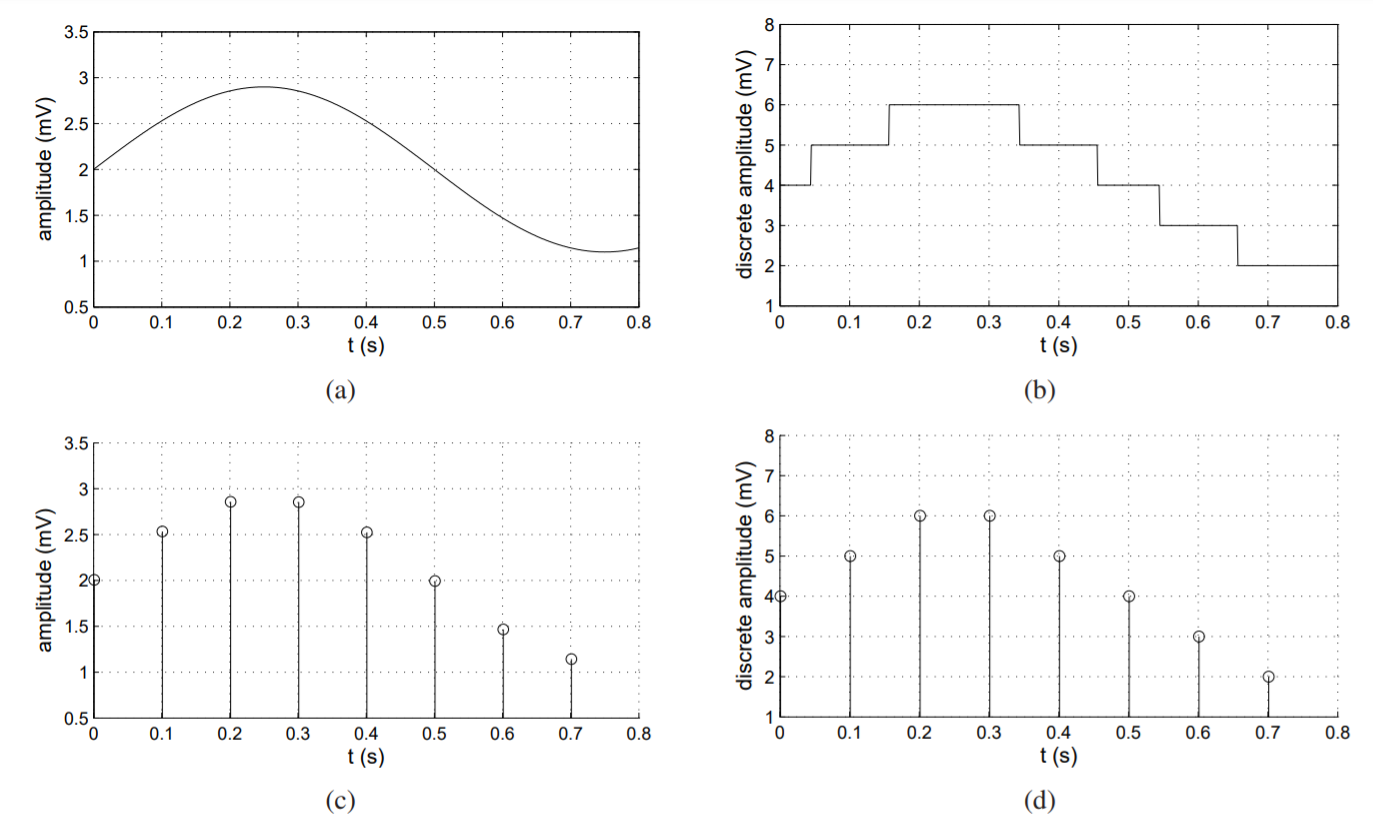
\includegraphics[scale=0.57]{img/signals.png}
		\captionsetup{margin=2cm}
		\caption{ (a) \textit{Analog}, (b) \textit{quantized-analog}, (c) \textit{sampled}, and (d) \textit{digital} signals. From \cite{avanzini2005fundamentals}.} 
		\label{fig:signals}
	\end{center}
\end{figure}
\noindent Furthermore, we can distinguish \textit{one-dimensional} and \textit{multi-dimensional} signals depending on the vector space dimension of $\mathcal{A}$. In particular, a signal is called one-dimensional if its value is a function of a single independent variable. An example of this class of signals is the audio, which is function of time. On the other hand, if the signal is a function of M independent variables, the signal is called a M-dimensional one. For example, images are function of two spatial coordinates. \\
Another distinction can be made between \textit{single-channel} and \textit{multi-channel} signals. Examples of the former category are mono recordings or black and white images, while stereo audio clips and RGB digital images are examples of the latter. In this thesis project we work mainly on single-channel, one-dimensional signals.

\subsection{From Analog to Digital} \label{from_a_to_d}
As previously motivated, this work deal mainly with digital signals. That means they are a sequence of data bits, obtained through a process that allows to convert signals from their original analog form to a digital one. According to \cite{proakis2006dimitris}, this procedure is called \gls{ad} conversion, and the corresponding devices are called \gls{ad} converters. \\
It is possible to divide this process into three main steps:
\begin{enumerate}
	\item \textit{Sampling}. This is the conversion of a continuous-time signal into a discrete-time one.
	\item \textit{Quantization}. It is basically an approximation process that consists in converting a continuous-valued signal into a discrete-valued one.
	\item \textit{Coding}. In this process, each discrete value is represented by a b-bit binary sequence.
\end{enumerate}
This section aims to deepen these three steps, since they are fundamental in plenty of \gls{dsp} applications. The main reference for this explanation is \cite{proakis2006dimitris}. \\
As previously mentioned, sampling is the first step of the \gls{ad} conversion.
This can be done in many ways, but in many practical applications a discrete-time signal $x(n)$ is obtained by a \textit{periodic}
or \textit{uniform} sampling of analog signals. If we denote with $x_{a}(t), \quad-\infty<n<\infty$ the analog signal, then the discrete-time signal can be calculated as follows:
\begin{align}\label{eq:from_a_to_d}
	\begin{array}{c}
		x(n)=x_{a}(nT), \quad-\infty<n<\infty
	\end{array}
\end{align}
\noindent where $T$ are the seconds between successive samples. This time interval $T$ is called the \textit{sampling period} or \textit{sample interval} and its reciprocal $1 / T=F_{s}$ is called the \textit{sampling rate} (samples per second) or the \textit{sampling frequency}, that is commonly measured in \gls{hz} (cycles per second). Equation \ref{eq:from_a_to_d} establishes a linear relationship between the time variables $t$ and $n$, that can be expressed as:
\begin{equation}\label{eq:tn_relation}
	t=n T=\frac{n}{F_{s}}
\end{equation}
\noindent A graphical example of the periodic sampling is given in Figure \ref{fig:periodic_sampling}.
\begin{figure}[H]
	\begin{center}
		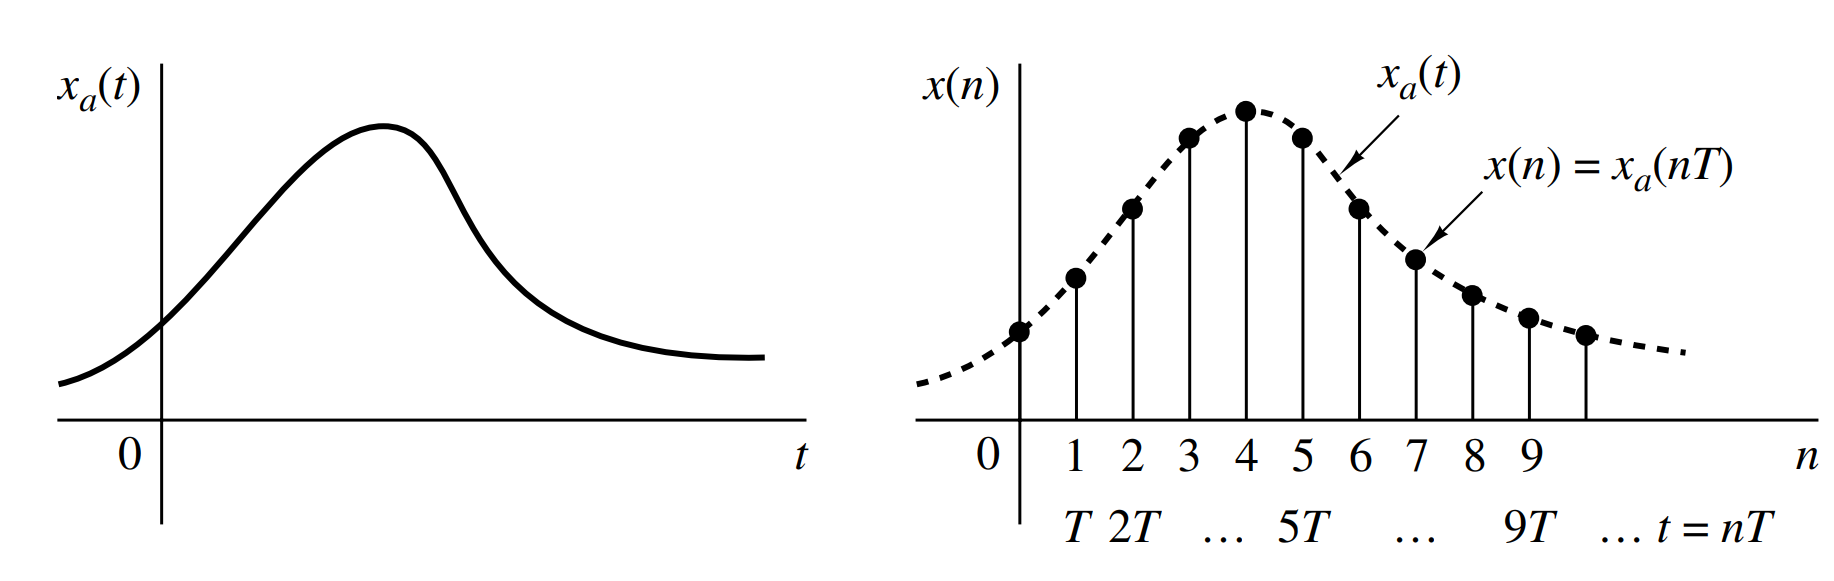
\includegraphics[scale=0.42]{img/periodic_sampling.png}
		\captionsetup{margin=2cm}
		\caption{ Periodic sampling of an analog signal. From \cite{proakis2006dimitris}.} 
		\label{fig:periodic_sampling}
	\end{center}
\end{figure}
\noindent At this point, it is important to point out how the sampling rate $F_s$ is selected in real \gls{dsp} applications. The acquisition of analog signals is typically driven by some prior knowledge about the characteristics of the signal to be sampled. In particular, this information concern the frequency content of general class of signals (e.g., the class of speech signals, the class of video signals, etc.), and they are generally available. For example, we know that human voice frequencies are, for the most part, below 3000 \gls{hz}. By knowing this information, appropriate sampling rate can be selected to avoid the problem commonly called \textit{aliasing}.\\
The latter occurs when the sampling rate is not sufficiently high to capture the higher frequencies of the original signal. The most common criterion to determine the sampling rate necessary to convert analog data to digital is given by the \textit{sampling theorem}, which was introduced by Nyquist (1928) and later popularized by Shannon (1949). This popular theorem states that it is possible to completely recover an analog signal $x_a(t)$ from its sample values if:
\begin{align}\label{eq:sampling_theorem}
	\begin{array}{c}
		F_s > 2\times F_{max}
	\end{array}
\end{align}
\noindent where $F_{max}$ is the largest frequency component in the analog signal. It is important to note that minimal sampling frequency that allows perfect reconstruction of a bandlimited signal from its samples, corresponds to $2\times F_{max}$. This sampling frequency is known as \textit{Nyquist rate}.\\ Thus, if the sampling rate is chosen according to the sampling theorem it is possible to avoid the problem of aliasing. A graphical example of the aliasing effect is given in Figure \ref{fig:aliasing}.

\begin{figure}[H]
	\begin{center}
		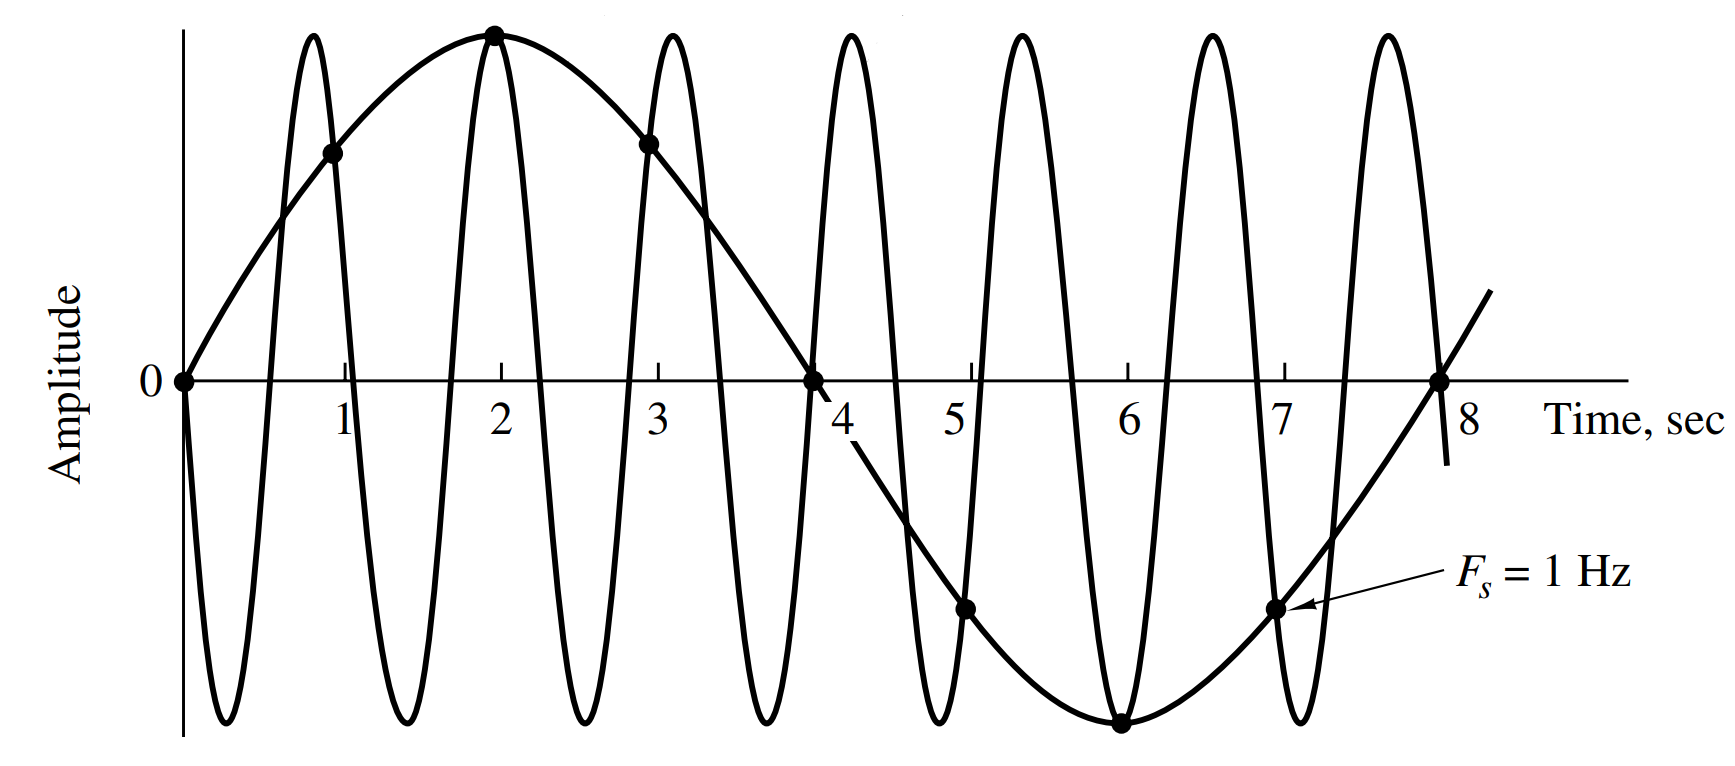
\includegraphics[scale=0.4]{img/aliasing.png}
		\captionsetup{margin=2cm}
		\caption{ Illustration of aliasing; the sampling frequency $F_{s} = 1$ \gls{hz} is not sufficiently high to unambiguously reconstruct the original sinusoid. From \cite{proakis2006dimitris}.} 
		\label{fig:aliasing}
	\end{center}
\end{figure}

\noindent Usually, after the sampling process, the quantization is performed. Briefly, quantization is the irreversible operation of converting a discrete-time continuous-amplitude signal into a digital one by expressing each sample value as a finite (instead of an infinite) number of digits. This results in signal distortion: it introduces the so called \textit{quantization error} which measures the difference between the quantized values and the actual sample ones. \\
Formally, let $x_{q}(n)$ denote the sequence of quantized samples at the output of the quantizer $Q[x(n)]$. Hence
\begin{align}\label{eq:quantizer}
	\begin{array}{c}
		x_{q}(n)=Q[x(n)]
	\end{array}
\end{align}

\noindent Then it is possible to define the quantization noise $e_{q}(n)$ as follows: 
\begin{equation}\label{eq:quant_noise}
	e_{q}(n)=x_{q}(n)-x(n)
\end{equation}
At this point, we can take an example to explain both the sampling and quantization processes more explicitly. First, consider the analog exponential signal
$$
x_a(t)=\left\{\begin{array}{ll}
	0.9^{t}, & t \geq 0 \\
	0, & t<0
\end{array}\right.
$$
\noindent Let $x(n) = 0.9^{n}, n \geq $ be the discrete-time signal obtained by the sampling process with $F_s = 1$ \gls{hz} (see Fig. \ref{fig:quantization} (a)). The resulting samples of $x(n)$ are shown in Table \ref{tab:quant}. As we can see, in this example, a complete description of the sampled signal requires $n$ significant digits. A precise description of each digit would be computationally heavy for most computers, and useless for many real applications. Thus, excess digits can be discarded by rounding the resulting number, as we can see in Figure \ref{fig:quantization} (b) and in Table \ref{tab:quant}. It is important to mention that the distance $\Delta$ between two successive quantized values is called \textit{quantization step}. 
\begin{figure}[]
	\begin{center}
		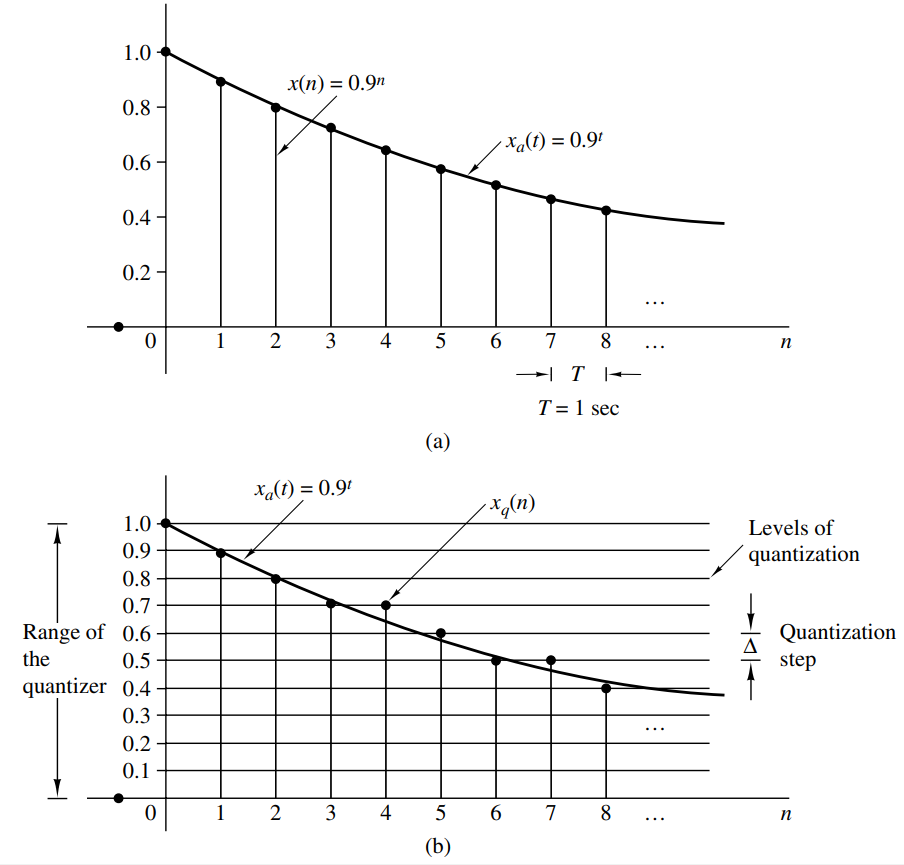
\includegraphics[scale=0.8]{img/quantization.png}
		\captionsetup{margin=2cm}
		\caption{Graphical example of quantization. From \cite{proakis2006dimitris}.} 
		\label{fig:quantization}
	\end{center}
\end{figure}

\begin{table}[]
	\begin{center}
		\begin{tabular}{clcl}
			\hline & $x(n)$ & $x_{q}(n)$ & $e_{q}(n)=x_{q}(n)-x(n)$ \\
			$n$ & Discrete-time signal & (Rounding) & Quantization Error \\
			\hline 0 & 1 & 1.0 & 0.0 \\
			1 & 0.9 & 0.9 & 0.0 \\
			2 & 0.81 & 0.8 & -0.01 \\
			3 & 0.72 & 0.7 & -0.029 \\
			4 & 0.6561 & 0.7 & 0.0439 \\
			5 & 0.59049 & 0.6 & 0.00951 \\
			6 & 0.531441 & 0.5 & -0.031441 \\
			7 & 0.4782969 & 0.5 & 0.0217031 \\
			8 & 0.43046721 & 0.4 & -0.03046721 \\
			9 & 0.387420489 & 0.4 & 0.012579511 \\
			\hline
		\end{tabular}
		\caption{Numerical illustration of quantization with one significant digit using rounding. From \cite{proakis2006dimitris}.}
		\label{tab:quant}
	\end{center}
\end{table}

\noindent As previously mentioned, the last step of \gls{ad} converters consists in the coding process. Thus, each sample is changed to an n bit code, such that each quantization level is assigned to a unique binary number.

\subsection{About Sinusoids}
Sinusoids are the building block of signal processing. As is described later in this chapter, all signals can be decomposed into constituent sinusoids of different frequencies using Fourier analysis. \\
Formally, it is possible to express a discrete-time sinusoidal signal as:
\begin{align} \label{eq:sinusoidal_signal}
	x(n) = A \sin(\omega n + \phi) = A \sin(2\pi fn + \phi) = A \sin(\frac{2\pi}{\tau}n + \phi), \qquad -\infty < n < \infty
\end{align}
\noindent The above definition introduces the following parameters \cite{christensen2019sound}:
\begin{itemize}
	\item The amplitude $A$, which scales the range of values of the sinusoid from  $[{-1},1]$ to  $[{-A},A]$.
	\item The frequency $\omega$ in radians per sample. Note that $\omega = 2 \pi f$, where $f$ is the frequency in cycles per sample. The frequency is inversely proportional to the period $\tau = \frac{1}{f}$, which measures the time the sinusoids takes to perform an entire cycle. 
	\item $\phi$ is the phase in radians. It can be thought of as a time-shift of the sinusoid.
\end{itemize}

\noindent It is important to note that sine and cosine are orthogonal waveform functions, i.e. they are out of phase by $\phi = \frac{\pi}{2}$. Therefore, from a terminological point of view, we refer to both cosine and sine functions as simply sinusoids. \\
A graphical example of a discrete-time sinusoid is given in Figure \ref{fig:sinusoidal_signal}.

\begin{figure}[H]
	\begin{center}
		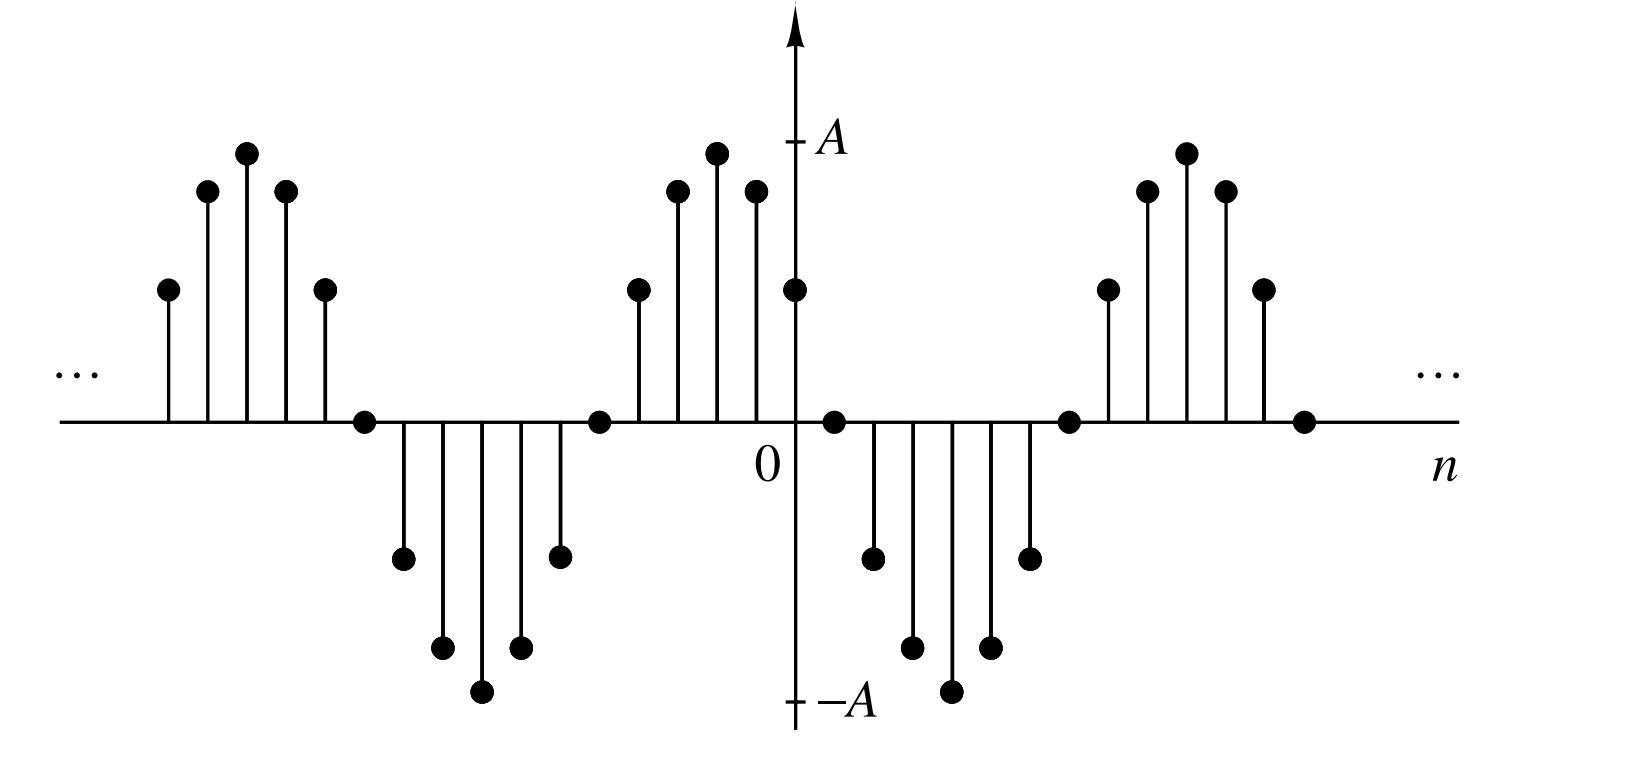
\includegraphics[scale=0.4]{img/sinusoidal_signal.png}
		\captionsetup{margin=2cm}
		\caption{Example of a discrete-time sinusoidal signal ($\omega = \frac{\pi}{6}$ and $\phi = \frac{\pi}{3}$). From \cite{proakis2006dimitris}.} 
		\label{fig:sinusoidal_signal}
	\end{center}
\end{figure}

\noindent It can be demonstrated  (see \cite{proakis2006dimitris}) that discrete-time sinusoids are characterized by the following properties:
\begin{itemize}
	\item A discrete-time sinusoid is periodic only if $f\in \mathbb{Q}$.
	\item Discrete-time sinusoids whose frequencies are separated by an integer multiple of 2$\pi$ are identical. From this property it follows that any sinusoid with a frequency $|\omega| > \pi$, or $|f| > \frac{1}{2}$, is an alias of a corresponding sequence resulting from a sinusoid with frequency $|\omega| < \pi$. For this reason, the range $0 \leq \omega \leq 2\pi$ or $-\pi \leq \omega \leq \pi$  ($0 \leq f \leq 1$, $-\frac{1}{2} \leq f \leq \frac{1}{2}$ ) is commonly defined as the \textit{fundamental range}.
	\item The highest rate of oscillation in a discrete-time sinusoid is attained when $|\omega| = \pi$ or, equivalently, $|f| = \frac{1}{2}$.
\end{itemize}

\subsubsection{Complex sinusoids}
\textit{Complex sinusoids}, (or \textit{complex exponentials}) are the building blocks of any real-world signal: as it is stated in Section \ref{fourier}, it is possible to decompose (or, at least, approximate) most signals of practical interest as a weighted sum of complex exponentials. Thus, it is important to introduce the class of these complex objects. \\
According to \cite{proakis2006dimitris}, we can define a complex exponential $x(n)$ as:
\begin{align}
	x(n) =  A e^{j(\omega n + \phi)} = A \cos(\omega n + \phi) + j A \sin(\omega n + \phi), \qquad -\infty < n < \infty
\end{align}
\noindent where $A$ is the amplitude and $j \in \mathbb{C}$ is the \textit{imaginary unit}. The link between exponential and trigonometric form of the above relation derives from the Euler identity, which is expressed as follows.
\begin{align}
e^{\pm j \theta}=\cos \theta \pm j \sin \theta
\end{align}

\subsection{Classification of Discrete-Time Signals}
The techniques used in \gls{dsp} depend heavily on the characteristics of the signal. Consequently, it is important to categorize signals based on their attributes. According to \cite{proakis2006dimitris}, important classes of discrete-time signals are the following.
\begin{itemize}
	\item \textit{Energy signals}. Consider a discrete-time signal $x(n)$, and let define the energy $E$ as:
	\begin{align}
		E =\sum_{n = -\infty}^{\infty} |x(n)|^2
	\end{align}
	If $E$ is finite, then $x(n)$ is an energy signal.
	\item \textit{Power signals}. The average power of $x(n)$ can be defined as:
	\begin{align}
	P=\lim _{N \rightarrow \infty} \frac{1}{2 N+1} \sum_{n=-N}^{N}|x(n)|^{2}
	\end{align}
	If $P$ is finite, then $x(n)$ is an energy signal.	Note that if $E$ is finite, $P = 0$, but if $E$ is infinite, $P$ may be either finite or infinite.
	\item \textit{Periodic signals}. A discrete-time signal $x(n)$ is periodi with period $N (N>0)$ if:
	\begin{align}
		x(n + N) = x(n) \qquad \forall n
	\end{align}
	The smallest value of $N$ for which this statement is true is called the fundamental period. It can be demonstrated (see \cite{proakis2006dimitris}) that  periodic signals are power signals. On the other hand, it is also worth noting that the energy of a periodic signal over a single period is finite if $x(n)$ takes on finite values over the period. 
	\item {Even and odd signals}. An even (or symmetric) signal $x(n)$ can be defined as a sequence with the following property:
	\begin{align}
		x(-n) = x(n)
	\end{align}
	On the other hand, a signal $x(n$) is called odd (or, equivalently, antisymmetric) if:
	\begin{align}
		x(-n) = -x(n)
	\end{align}
	Graphical examples of symmetric and antisymmetric signals are given, respectively, in Figure \ref{fig:evenodd} (a) and (b).
	\begin{figure}[H]
		\begin{center}
			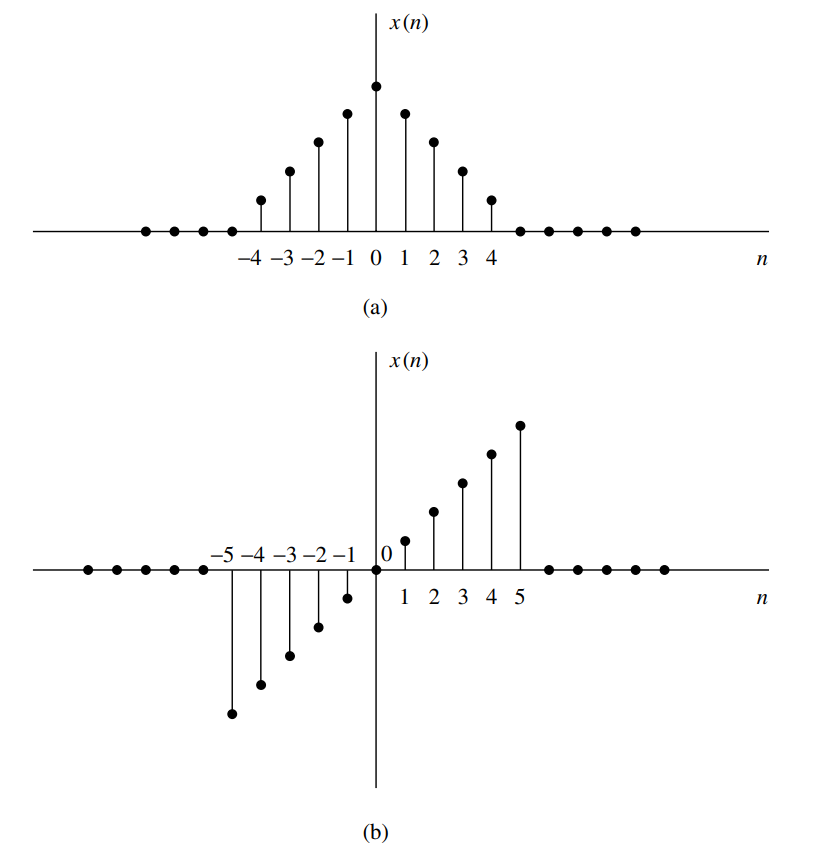
\includegraphics[scale=0.8]{img/evenodd.png}
			\captionsetup{margin=2cm}
			\caption{Example of even (a) and odd (b) signals. From \cite{proakis2006dimitris}.} 
			\label{fig:evenodd}
		\end{center}
	\end{figure}
\end{itemize}

\subsection{Spectral Analysis of Signals} \label{fourier}
Frequency analysis is a powerful tool that is widely used in a large variety of engineering and signal processing tasks. Briefly, the spectral representation aims to highlight how the energy is distributed across frequency components of the signal. Furthermore, the spectral representation is particularly suited for performing specific classes of operations, such as the convolution. \\
As previously mentioned, signals can be decomposed into a weighted sum of sinusoidal signal components (or complex exponentials). The decomposition techniques depend on the characteristic attributes of the specific signal. Indeed, there are frequency analysis tools that apply only to specific families of signals. In particular, periodic signals can be decomposed through \textit{Fourier series}; on the other hand, for the class of finite energy signals, the decomposition is called the \textit{Fourier transform}. \\
This section aims to explain the difference between these tools, by referring mainly to the book \cite{proakis2006dimitris}. Since this project deals only with digital signals, only definitions concerning discrete time-signals are discussed.
\subsubsection{Discrete-Time Fourier Series}
\textit{Fourier series} are used to decompose periodic sequences into a weighted sum of frequency components. Formally, suppose to have a discrete-time  periodic signal $x(n)$ with period $N$ such that $x(n)=x(n+N)\quad\forall n$. The Fourier series for that signal can be expressed as:
\begin{align}\label{Synthesis_eq_fs}
x(n)=\sum_{k=0}^{N-1} c_{k} s_{k}(n)
\end{align}
where {$c_k$} are the coefficients in the series representation and $s_{k}$ consists of $N$ harmonically related exponential functions, such that:
\begin{align} \label{harmonic}
s_k(n) = e^{j 2 \pi n \frac{k} {N}}, \qquad k=0,1, \ldots, N-1
\end{align}
The set defined in \ref{harmonic} is composed of periodic complex exponentials which share fundamental frequencies that are multiples of a single positive frequency term. It is noticeable that, from a terminological point of view, the sequence $s_k(n)$ is called the k-th \textit{harmonic} of $x(n)$.\\
The relationship \ref{Synthesis_eq_fs} is called \textit{Synthesis equation} or, equivalently, \gls{dtfs}. As for the Fourier coefficients $c_k$, they represents the amplitude and phase associated with the frequency component $s_k(n)$. In other words, these coefficients provide the description of the periodic signal $x(n)$ in the frequency domain. Their definition is provided by the \textit{Analysis equation} expressed in \ref{analysis_eq_fs}.
\begin{align}\label{analysis_eq_fs}
	c_{k}=\frac{1}{N} \sum_{n=0}^{N-1} x(n) e^{\frac{-j 2 \pi kn} {N}}, \qquad k=0,1, \ldots, N-1
\end{align}
\noindent Furthermore, it can be demonstrated that the spectrum of a periodic signal $x(n)$ with period $N$, is a periodic sequence with period $N$. Consequently, it is sufficient to observe any $N$ consecutive samples belonging to the signal in either time or frequency domain to provide its complete description.\\
Lastly, it is important to highlight that real periodic signals have interesting  symmetry properties. In particular, we know that for a real periodic signal, the spectral magnitude has an even symmetry property, such that: 
$$
|c_{-k}| = |c_k|
$$
As for the spectral phase, we know that:
$$
\measuredangle  c_{-k}= \measuredangle c_{k} \quad
$$
As a direct consequence of these properties, we can conclude that it is possible to specify the whole signal in the frequency domain by taking into account only $\lfloor \frac{N}{2} \rfloor$ consecutive values. 

\subsubsection{Discrete-Time Fourier Transform} %Discrete-Time Fourier Transform?
Aperiodic signals can be decomposed through Fourier Transforms. From the \gls{dsp} theory \cite{proakis2006dimitris} we know that, given a discrete-time signal $x(n)$ with finite energy, it is possible to represent its frequency content by the analysis equation \ref{eq:analysis dtft}.

\begin{align}\label{eq:analysis dtft}
X(\omega)=\sum_{n=-\infty}^{\infty} x(n) e^{-j \omega n} = \sum_{n=-\infty}^{\infty} x(n) e^{-j 2 \pi f n}
\end{align}

\noindent From a notational point of view, we can write that:
$$
x(n) \stackrel{\mathscr{F}}{\longleftrightarrow} X(\omega)
$$
to denote that $X(\omega)$ is the Fourier Transform of $x(n)$.\\
The formula in \ref{eq:analysis dtft} is also called \gls{dtft}. From a conceptual point of view, $X(\omega)$ represents the decomposition of $x(n)$ into its frequency components. \\
As in the case of \gls{dtfs}, we can define a synthesis equation (\ref{eq:synthesis dtft}) too.
\begin{align}\label{eq:synthesis dtft}
x(n)=\frac{1}{2 \pi} \int_{2 \pi} X(\omega) e^{j \omega n} d \omega = \frac{1}{2 \pi} \int_{-\pi}^{\pi} X(\omega) e^{j \omega n} d \omega 
\end{align}
\noindent It is worth noting that, since \gls{dtft} is a periodic function of the frequency variable $\omega$, it has a Fourier series expansion. Therefore, its Fourier coefficients are the values of $x(n)$. In other words, the synthesis equation just written can be considered as an analysis equation of the Fourier Series of $X(\omega)$. In fact, the \gls{dtft} of $x(n)$ results in a periodic signal, with period $2\pi$. This is demonstrated below.
$$
X(\omega+2\pi k) =\sum_{n=-\infty}^{\infty} x(n) e^{-j(\omega+2 \pi k) n} = \sum_{n=-\infty}^{\infty} x(n) e^{-j \omega n} e^{-j 2 \pi k n} =\sum_{n=-\infty}^{\infty} x(n) e^{-j \omega n}=X(\omega)
$$
\noindent Also in this case there are some important symmetry properties. It is possible to demonstrate (\cite{proakis2006dimitris}) that if $x(n)$ is real, then:
$$|X(-\omega)|=|X(\omega)| \qquad \text{(even symmetry)}
$$
$$
\measuredangle X(-\omega)=- \measuredangle X(\omega), \quad \text { (odd symmetry) }$$
From these relations, we can conclude that it is possible to determine the frequency content of $x(n)$ from the range of values $0 \leq f \leq \frac{1}{2}$ (or, equivalently $0 \leq \omega \leq \pi$) rather than $-\frac{1}{2} \leq f \leq \frac{1}{2}$ ($-\pi \leq \omega \leq \pi$). In other words, if we know $X(-\omega)$ in the range $0 \leq \omega \leq \pi$  we can calculate $X(-\omega)$ over $-\pi \leq \omega < 0$. Summing up, the whole description of a discrete-time real signal $x(n)$ in the frequency domain is determined over the continuous range of values $0 \leq \omega \leq \pi$.

\subsubsection{Discrete Fourier Transform}
The \gls{dft} is a computational tool that plays a very important role in a wide variety of \gls{dsp} applications, such as linear filtering, spectrum analysis and power frequency estimation. \\
As previously motivated, Fourier transform aims to perform frequency analysis of a signal by decomposing it into different frequency components. Such a spectral representation leads to a discrete function in the case of \gls{dtfs}, i.e. when the input $x(n)$ is periodic. On the other hand, \gls{dtft} on aperiodic signals is a continuous function of frequency; therefore, from a computational point of view, it is not a convenient representation of the signal spectrum. \\
For this reason, it is important to introduce \gls{dft}, which is a powerful tool for representing a signal in the spectral-domain in a computationally efficient manner. \\
Formally, if we have a signal $x(n)$ of length $N$, it is possible to represent its frequency content with the following equation.

\begin{align}\label{eq:dft}
	X(k) =\sum_{n=0}^{N-1} x(n) e^{-j \frac{2 \pi k n}{N}}, \quad k=0,1,2, \ldots, N-1 
\end{align}

\noindent Conceptually, the \gls{dft} relation in \ref{eq:dft} expresses the Fourier transform as a function of a $N$-length equally spaced set of discrete frequencies. Indeed, it is possible to observe that the function is parametrized by the use of a discrete variable $k \in [0,N] \subset \mathbb{Z}$ rather than a continuous one $\omega\in [0,2\pi] \subset \mathbb{R}$.\\
The signal $x(n)$ can be recovered from its frequency samples by the $N$-point \gls{idft} relation in \ref{eq:idft}. 
\begin{align}\label{eq:idft}
	x(n) = \frac{1}{N} \sum_{n=0}^{N-1} X(k) e^{j \frac{2 \pi k n}{N}}, \quad n=0,1,2, \ldots, N-1
\end{align}
\noindent It is possible to demonstrate (see \cite{proakis2006dimitris}) that if we have a finite-duration sequence $x(n)$ of length $N_{lim}<N$, then the \gls{idft} yields $x(n) = 0 \text{ for } N_{lim} \leq n \leq{N-1}$. Otherwise, if the sequence $x(n)$ is time-limited by a value $N_{lim}$ such that $N_{lim}>N$, the $N$-point \gls{idft} results in an aliased version of the original signal. \\
\gls{dft} is a powerful tool which has many properties. The objective of this section is not to provide an exhaustive analysis of these properties, for which we refer to excellent textbooks (such as \cite{proakis2006dimitris}); thus, our aim is to determine only the properties linked to real-valued sequences, since they are of fundamental importance for the developed models (as it is explained in Chapter \ref{chap:methods}).\\
In this regard, if $x(n)$ is real, then 
$$|X(N-k)|=|X(k)|$$ 
$$\angle X(N-k)=-\angle X(k)$$
Furthermore, it can be demonstrated that $x_{I}(n)= 0$.\\
Finally, it is important to mention that the importance of \gls{dft} and \gls{idft} operations is enhanced by the fact that there are computationally efficient procedures, such as the family of \gls{fft} algorithms, from which they can be performed. The computational complexity of these algorithms depends on whether or not the input signal has some specific attributes (such as the symmetry for real-valued sequences already described).

\subsection{Discrete-time Systems}
In \gls{dsp} terminology, each physical device or digital algorithm that performs some operation on signals is called \textit{system}. As previously motivated, when we work with data on a computer, time is discretized, so that each operation is performed on discrete-time signals. For this reason, we focus our attention on discrete-time systems, i.e. devices or algorithms that operate on a discrete-time signal. \\
Formally, we can define a system $S$ as a set of operations performed on the input (or \textit{excitation}) signal $x(n)$ to produce the output (or \textit{response}) signal $y(n)$. Figure \ref{fig:dtsystem} illustrates this definition. \\
\begin{figure}[]
	\begin{center}
		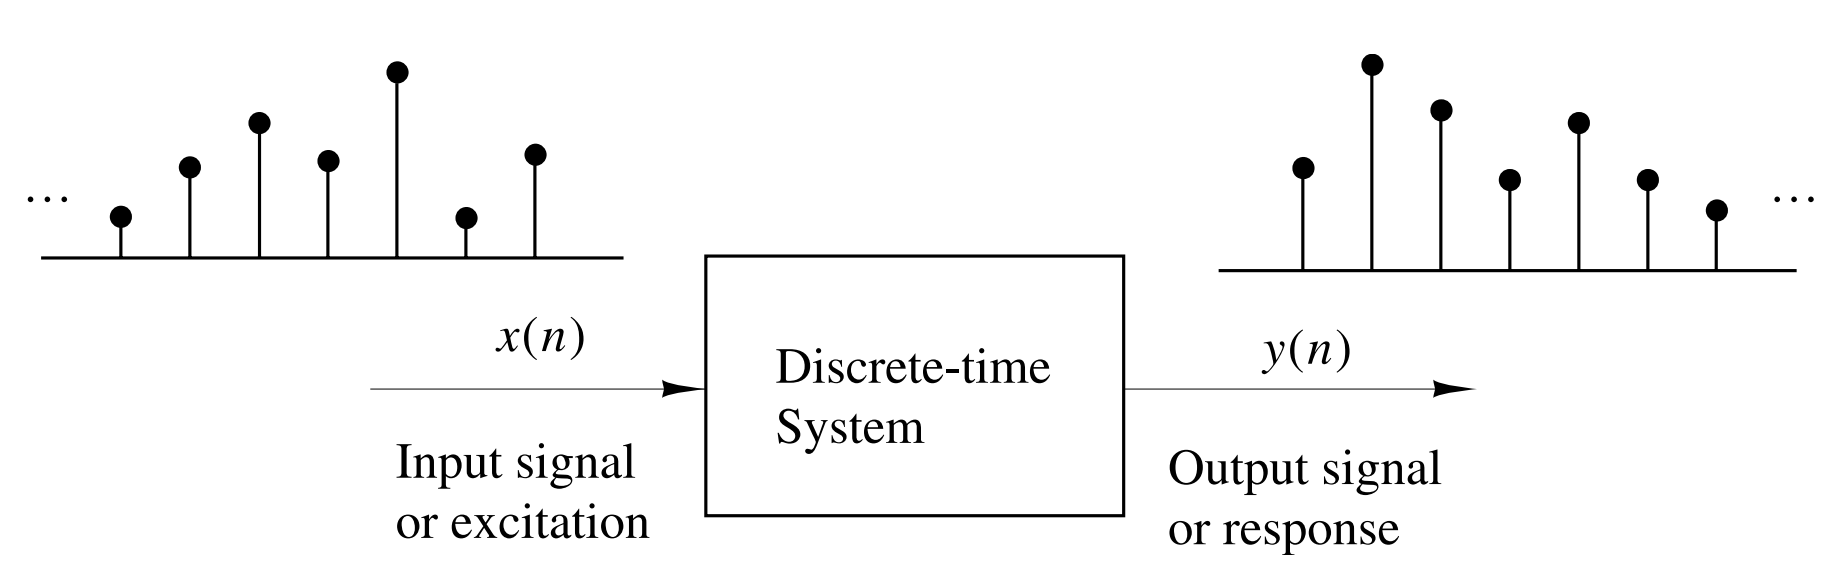
\includegraphics[scale=0.4]{img/dtsystem.png}
		\captionsetup{margin=2cm}
		\caption{Block diagram representation of a discrete-time system. From \cite{proakis2006dimitris}.} 
		\label{fig:dtsystem}
	\end{center}
\end{figure}
\noindent We can use equivalently the following two notations to express the transformation from $x(n)$ to $y(n)$ by the system $S$.
\begin{align}
	x(n) \xrightarrow{\text{S}} y(n)
	y(n) = S(x(n))
\end{align}
\noindent For our analysis purposes, as well as for providing a comprehensive
overview of the basic \gls{dsp} principles, it is important to classify systems according to their characteristics. In fact, the mathematical operations performed in this study are heavily dependent on the properties that the system satisfies. \\
According to \cite{proakis2006dimitris}, important classes of discrete-time systems are the following.

\begin{itemize}
	\item \textit{Time-invariant systems}. A system is called time-invariant if its input–output description $x(n) \xrightarrow{\text{S}} y(n)$ do not changes with time. Formally, let $x(n)$ be the input of a system $S$; if 
	$$y(n, k) = y(n - k) \quad \forall k$$
	where  $y(n, k) = S[x(n-k)]$, then $S$ is a time-invariant system. 
	\item \textit{Linear systems}. A system is said to be linear if it satisfies the principle of \textit{superposition}, which is formally described below. Given two arbitrary input sequences $x_1(n), x_2(n)$ and two arbitrary constants $a_1, a_2$ a system $S$ is linear if and only if:
	\begin{align}
		S[a_1x_1(n) + a_2x_2(n)] = a_1S[x_1(n)] + a_2S[x_2(n)] \qquad \forall x_1(n), x_2(n), a_1, a_2 
	\end{align}
	The above definition includes two important properties of linear systems: multiplicative and additive.
	\item \textit{Causal system}. A system called causal if its output depends only on present and past inputs	but does not depend on future ones. Formally, $S$ is causal if: 
	\begin{align}
		y(n) = F[x(n), x(n-1), x(n-2), ...]
	\end{align}
	where $F[.]$ is some arbitrary function. \\
	It is quite intuitive that causal system are at the basis of real-time \gls{dsp} applications, since the observation of input future values is  physically not possible. On the other hand, off-line processing often involves algorithms that perform \textit{non-causal} operations. A good example is provided by bi-directional \gls{rnn}s, which, for a given time step, process not only the past data elements in a given sequence, but also the future ones. 
\end{itemize}

\noindent Of particular importance for many \gls{dsp} applications is the class of \gls{lti} systems, whose response to an input sequence is determined by the \textit{convolution} operation. 


\subsubsection{Convolution}
Convolution is an important mathematical tool in both \gls{dsp} and \gls{dl} fields. In this section we introduce this operation from a theoretical perspective, while in paragraph \ref{cnns} its application in the context of neural networks is described. \\
In order to introduce the convolution, it is first important to define the \textit{unit sample sequence} (or \textit{unit impulse}), which corresponds to the most basic discrete-time signal. In particular, it is a signal that is zero everywhere, except at $n = 0$ where its value is unity. Formally:
\begin{align}
	\delta(n) = \begin{cases} 1 & \mbox{se } \mbox{ $n$ = 0} \\ 0 & \mbox{$ n\neq$ 0} \end{cases}  
\end{align}
\noindent Its graphical representation is provided in Fig. \ref{fig:unit}.
\begin{figure}[H]
	\begin{center}
		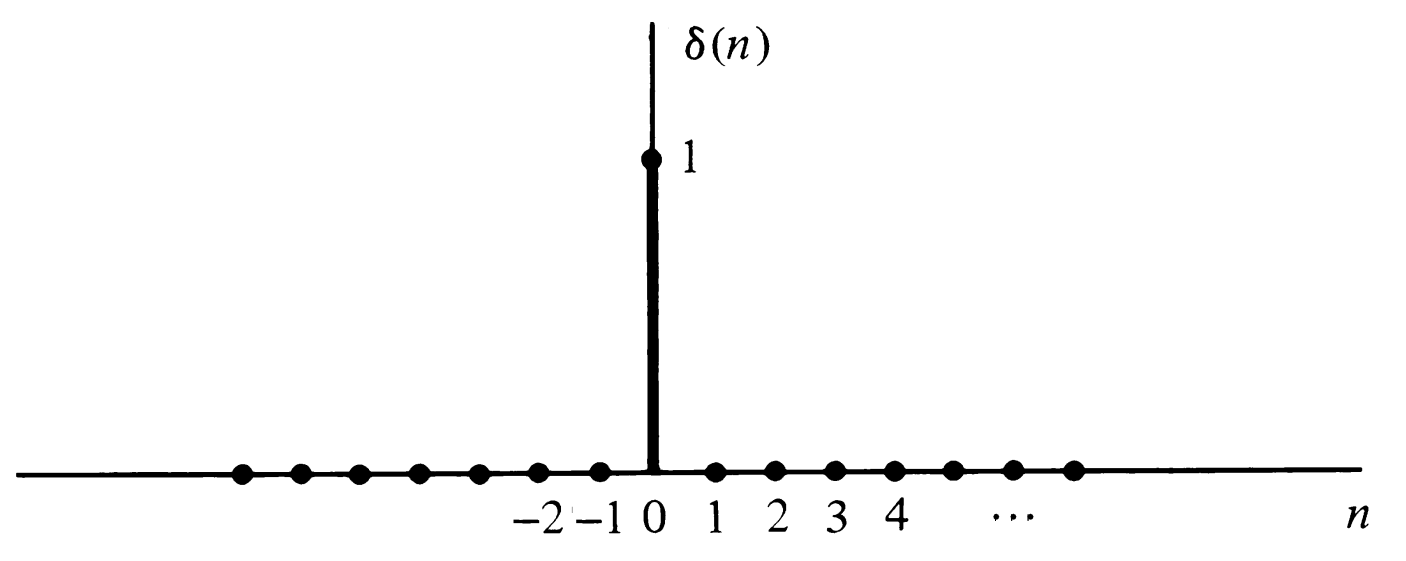
\includegraphics[scale=0.4]{img/unit.png}
		\captionsetup{margin=2cm}
		\caption{Graphical representation of
			the unit sample signal. From \cite{proakis2006dimitris}.} 
		\label{fig:unit}
	\end{center}
\end{figure}

\noindent At this point, it is possible to introduce the equation \ref{eq:decomposition_xn}, which expresses the decomposition of an arbitrary signal $x(n)$ into a weighted sum of shifted unit impulses.
\begin{align} \label{eq:decomposition_xn}
	x(n) =  \sum_{k = - \infty}^{\infty}x(k)\delta(n-k)
\end{align}
\noindent The importance of the relationship above expressed lies in the following considerations. \\
If we consider the response of a \gls{lti} system to $x(n)$ is the corresponding sum of weighted outputs, we obtain the expression \ref{eq:superp_summ}. 

\begin{align} \label{eq:superp_summ}
	y(n) = S[x(n)] = S\left[\sum_{k = - \infty}^{\infty}x(k)\delta(n-k)\right] =  \sum_{k = - \infty}^{\infty}x(k)S\left[\delta(n-k)\right]
\end{align}

\noindent Let now consider the unit sample signal $\delta(n)$ in a \gls{lti} system. We can denote as $h(n)$ the response of $S$ to this signal. Formally:
\begin{align} \label{eq:lti_resp}
	h(n) = S[\delta(n)]
\end{align}

\noindent The formula in \ref{eq:lti_resp} is of particular importance as it characterizes the system $S$: as stated in \cite{proakis2006dimitris}, \gls{lti} systems can be subdivided into FIR (finite-duration impulse response) and IIR (infinite-duration impulse response) depending on whether $h(n)$ has, respectively, finite or infinite duration. These concepts lie at the basis of the design of digital filters, for which we refer to the cited book.\\
Because of the system time-invariance property, it can be seen that:

\begin{align}
	h(n-k) = S[\delta(n-k)]
\end{align}

\noindent Consequently, the formula in \ref{eq:superp_summ} reduces to:
$$
	y(n) = \sum_{k = - \infty}^{\infty}x(k)h(n-k)
$$

\noindent which is called \textit{convolution sum} and can be better expressed with the following notation: 
\begin{align} \label{eq:conv_sum}
x(n) \circledast h(n) = y(n) = \sum_{k = - \infty}^{\infty}x(k)h(n-k)
\end{align}

\noindent The previous result (formula \ref{eq:conv_sum}) asserts that the response of an \gls{lti} system to a given input signal is obtained by \textit{convolving} the input sequence $x(n)$ with the system's response $y(n)$ to the unit impulse $h(n)$. \\
Furthermore, it is important to mention that, in \gls{dl} terminology (see \cite{goodfellow2016deep}), the first argument (in our definition, the function $x$) to the convolution is called \textit{input}, while the second argument ($h$) is called \textit{kernel}. Furthermore, the output $y$ is sometimes referred to as the \textit{feature map}. \\
The convolution operation has some important properties:

\begin{itemize}
	\item \textit{Commutative law}:
	\begin{align} 
		y(n) = x(n) \circledast h(n) = h(n) \circledast x(n) = \sum_{k = - \infty}^{\infty}x(k)h(n-k) = \sum_{k = - \infty}^{\infty}h(k)x(n-k)
	\end{align}
	\item \textit{Associative law}:
	\begin{align}
		[x(n) \circledast h_1(n)] \circledast h_2(n) = x(n) \circledast [h_1(n) \circledast h_2(n)]
	\end{align}
	\item \textit{Distributive law}:
	\begin{align}
		x(n) \circledast [h_1(n) + h_2(n)] = x(n) \circledast h_1(n) +  x(n) \circledast h_2(n)
	\end{align}
\end{itemize}
\noindent The convolution operation is an important tool even when we analyze the frequency response to \gls{lti} systems. In particular, we know from the so called \textit{convolution theorem} that convolution in the time domain is equivalent to multiplication in the frequency domain. \\
Formally, let $X(\omega), H(\omega), Y(\omega)$ be the spectra of, respectively, $x(n), h(n), y(n)$; then, the theorem asserts that:
\begin{align} \label{conv_theorem}
	y(n)=x(n) \circledast  h(n) \stackrel{\mathscr{F}}{\longleftrightarrow} Y(\omega)=X(\omega) H(\omega)
\end{align}
\noindent From this theorem we can conclude that convolution is an easier operation in the time domain rather than in the frequency one. \\


\section{Deep Learning}
The term \textit{artificial intelligence} is increasingly used in a variety of ways and behind it, there are many technologies. Rai et. al \cite{rai2019editor}, provide a quite comprehensive definition. "\gls{ai} is typically defined as the ability of a machine to perform cognitive functions that we associate with human minds, such as perceiving, reasoning, learning, interacting with the environment, problem solving, decision-making, and even demonstrating creativity". Although this definition is rather generic, it is possible to define, more specifically, the disciplines that belong to it. \\
Most of the time, researchers refers to the term \gls{ai} to indicate \gls{ml} algorithms. We can consider \gls{ml} as the discipline that extracts patterns of interest from data \cite{goodfellow2016deep}. \\
Mitchell \cite{mitchell1997machine} provides a quite formal definition of \gls{ml}: “A computer program is said to learn from experience E with respect to some class of tasks T and performance measure P, if its performance at tasks in T, as measured by P, improves with experience E”.\\
\gls{ml} is a very active research topic and it has many practical applications. Thus, the task T can range from medical diagnosis and community detection to antispam filtering and text categorization. However, many problems can be roughly categorized into two groups: classification (such as speaker identification) and regression (such as audio \gls{sr}). \\
In order to evaluate the performance of a \gls{ml} algorithm, a quantitative measure must be taken into account. Mitchell refers to this metric, which is always specific to the task T, as performance measure P. 
As for the learning experience E, \gls{ml} algorithms can be broadly categorized in two main classes: \textit{superivsed} and \textit{unsuperivsed}. Briefly, supervised learning aims to generate reliable predictions using labeled data. In other words, a supervised learning algorithm experiences a dataset on which each example is associated with a so called "ground truth", which represents the real output the model should be able to reproduce (or, at least, approximate). Audio super-resolution is a good example of supervised learning, since the goal is to learn a function that accurately maps the input \gls{lr} sequences to the corresponding \gls{hr} audio frames. \\
On the contrary, in unsupervised learning, the ground truth is not available. Indeed, the learning process focuses on useful properties of the dataset structure. Most of the time, the goal is to learn the entire probability distribution that generated the data. \\
It is possible to define a third category, i.e. \textit{semi-supervised learning}. According to Hady and Schwenker \cite{hady2013semi}, this approach aims to maximize the performance of a \gls{ml} model by integrating part or all of the available unlabeled data in its supervised learning process. \\
There are several different approaches in \gls{ml}, depending on the task and the data. On one hand, many problems can be tackled by designing a specific set of features to extract. The feature extraction step is very important, since the performance of the \gls{ml} algorithms are highly sensitive to the representation of the input data. \\
On the other hand, in some cases, it is not possible - or at least, is very difficult - to extract representative features for a specific task. For example, in the field of digital signal processing, descriptive variables such as energy, mean, variance, etc$\dots$ are not always sufficient to detect distinctive patterns of interest. In this case, we can use specific \gls{ml} approaches that can discover the right features to solve the problem by using raw data. This \textit{representation learning} approach often results in much better performance than can be obtained with hand-crafted feature extraction. Furthermore, representation learning is a less-time consuming approach since there is a minimal human intervention. \\
As for \textit{Deep Learning}, we can consider it as a \gls{ml} sub-field, in which the features are extracted through increasingly abstract hidden layers. \gls{dl} aims to estimate the desired mapping function by breaking it into a series of hidden mappings, each described by a different layer which provides a new representation of the input. \gls{dl} models result in complex computational graphs whose interpretability is often poor. \\
A schematic illustration of the newly introduced concepts is shown in Fig.\ref{fig:ai}.
\begin{figure}[H]
	\begin{center}
		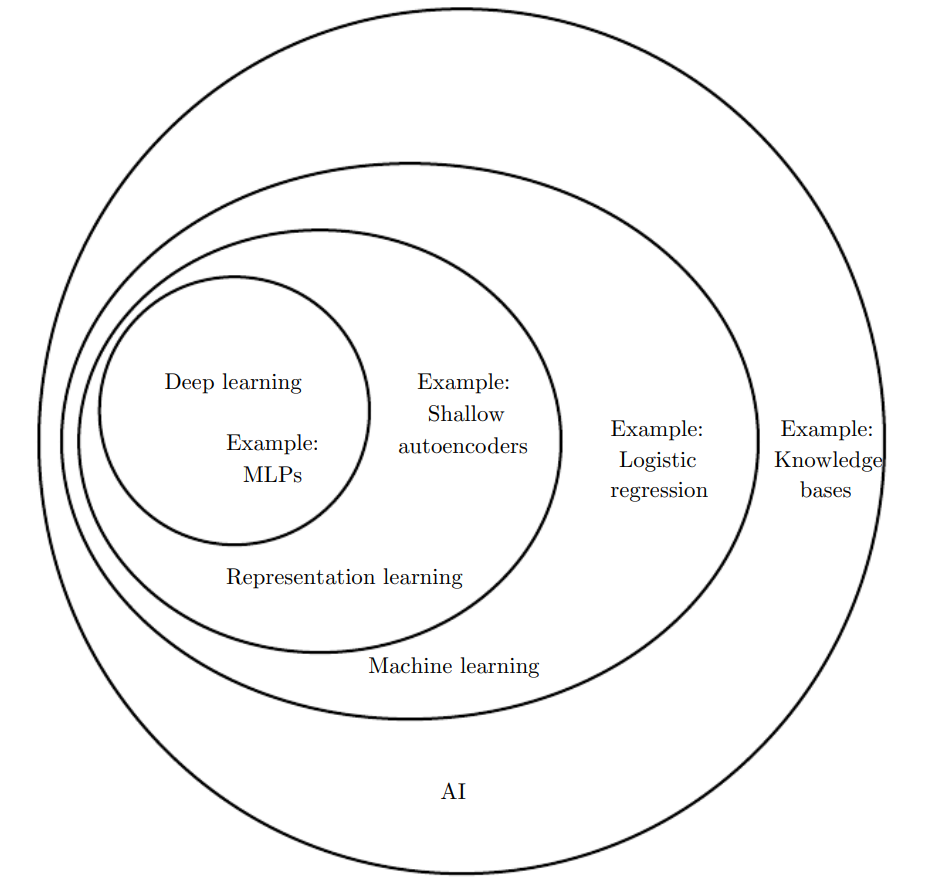
\includegraphics[scale=.7]{img/ai.png}
		\captionsetup{margin=2cm}
		\caption{A Venn diagram showing the conceptual location of \gls{dl},  \gls{ml} and \gls{ai} in the terms hierarchy. We can consider \gls{ai} as the term with the wider range of uses. Each section of the diagram includes an example of an \gls{ai} technology. From \cite{goodfellow2016deep}.}
		\label{fig:ai}
	\end{center}
\end{figure}
\noindent \gls{dl} is particularly effective when applied to large training sets, i.e. in high dimensional spaces with a large number of data points. Indeed, its use is perfectly suited for \gls{dsp} tasks, in which quite
a large amount of data is usually required. In this regard, it is noticeable that the popularity of deep-learning based approaches is largely due to their success in large-scale image classification tasks (see ImageNet \cite{ILSVRC15}). \\
There are many variants of deep-learning algorithms with different architectures and characteristics; some examples includes convolutional, generative and recurrent networks. The main objective of this section is to provide a broad description of these methodologies, trying to cover in a rather exhaustive way the main aspects that characterize them. A particular focus is given to convolutional and recurrent approaches, as they are of fundamental importance for the purposes of this work.

\subsection{The Learning Process} %o the learning process
As previously said, the task of Audio \gls{sr} belongs to the class of supervised learning problems; for this reason, we focus on the learning process, which is a central aspect that concerns this approach. \\
Briefly, supervised learning aims to learn a function $f_{\theta}$ that accurately maps input vectors $X$ to target labels $Y$. This formulation can be applied to a wide variety of problems; for example, we can see an audio \gls{sr} model as a mapping function of the form $f_{\theta}: X \rightarrow Y$ (see section \ref{problem_formulation}). \\
In order to measure how the function $f_{\theta}$ is accurate, we need to introduce the concept of \textit{objective function} also called \textit{loss function} or \textit{criterion}. We use these terms interchangeably though some researchers assign different meaning to some of these terms.\\
Formally, we can consider the criterion $L(\hat{y}, y)$ as a function which maps the model output $\hat{y}$ to a real number measuring the quality of the solution in terms of distance from the ground truth $y$. During the training phase, the parameters $\theta$ of the model are then set to optimize the loss. \\
Optimization in this case refers to the problem of minimizing (or, depending on the problem, maximizing) the objective function $L$ over the training samples. Proper solutions of the optimization problem can concern gradient-based methods; without going into that in detail, we only mention that these iterative optimization algorithms seeks to find the minimum (or the maximum) of a function by obtaining partial derivatives. Derivatives are important as they indicate on which direction each parameter of the model must be adjusted in order to reduce the error. \\
The most common optimization algorithms are Stochastic Gradient Descent \cite{kiefer1952stochastic}, Adam \cite{kingma2014adam}, Nadam \cite{dozat2016incorporating}, $\dots$ In all cases, the main idea is that, at each iteration, the loss function must be decreased by moving it in the direction of the negative gradient. The model parameters are then adjusted through the backpropagation algorithm \cite{amari1993backpropagation}. The convergence toward the minimum of the objective function model ~-~ and the speed of this convergence ~-~ depends upon the \textit{learning rate}, a positive scalar value. \\
For more details about these interesting aspects, as well as for a formal statement, we refer to the book "Deep Learning" \cite{goodfellow2016deep} by Goodfellow, Bengio and Courville. \\
As for loss functions, we mention, as typical examples, Negative Log-Likelihood, Cross-Entropy and \gls{mse}; the choice of which one to use is strongly influenced by the nature of problem. \\
A key aspects of optimization in \gls{dl} problems, is that loss functions are not necessarily convex. Ideally, we would obtain the global minimum, but this is not always possible, since there are multiple local minima and plateaus. For this reason, suboptimal solutions are generally accepted, as long as they correspond to significantly low values of the cost function.
\\
The main challenge of \gls{dl} (or, more generally, \gls{ml}) problems is that we must produce good predictions on unseen data. Indeed, according to \cite{goodfellow2016deep}, we can determine how well an algorithm performs by looking for its ability to both obtain a sufficiently low error value on the training set and minimize the gap between training and test error. Both abilities are of fundamental importance to avoid \textit{underfitting} and \textit{overfitting} problems. In particular, when the model is not able to make the training error small, we say it underfits. On the other hand, overfitting occurs when we measure a large gap between training and test error. The desired behavior occurs when the algorithm succeeds in learning the data distribution, providing good performance on the training set and, at the same time, can \textit{generalize} well on previously unobserved instances. \\
Underfitting and overfitting can be defined as function of two different sources of error: \textit{bias} and \textit{variance}. The former is a measure of the expected deviation of the estimator relative to the true value. From a statistical point of view, although unbiased estimators are desirable, since they have important properties, they are not always the best estimators. At the same time, a high bias can cause the underfitting. \\
On the other hand, variance measures the variability of the estimator about the expected value. If the model gets too sensitive to small variations of the data points during the learning phase, the generalisation capability can then be very poor (overfitting). \\
Therefore, when training a \gls{dl} model, it is important to take into account these aspects, as we aim to simultaneously minimize these two sources of error. This conflict is known in literature as "bias-variance trade-off". Figure \ref{fig:underoverfitting} provides a graphical representation of this problem. \\
\begin{figure}[H]
	\begin{center}
		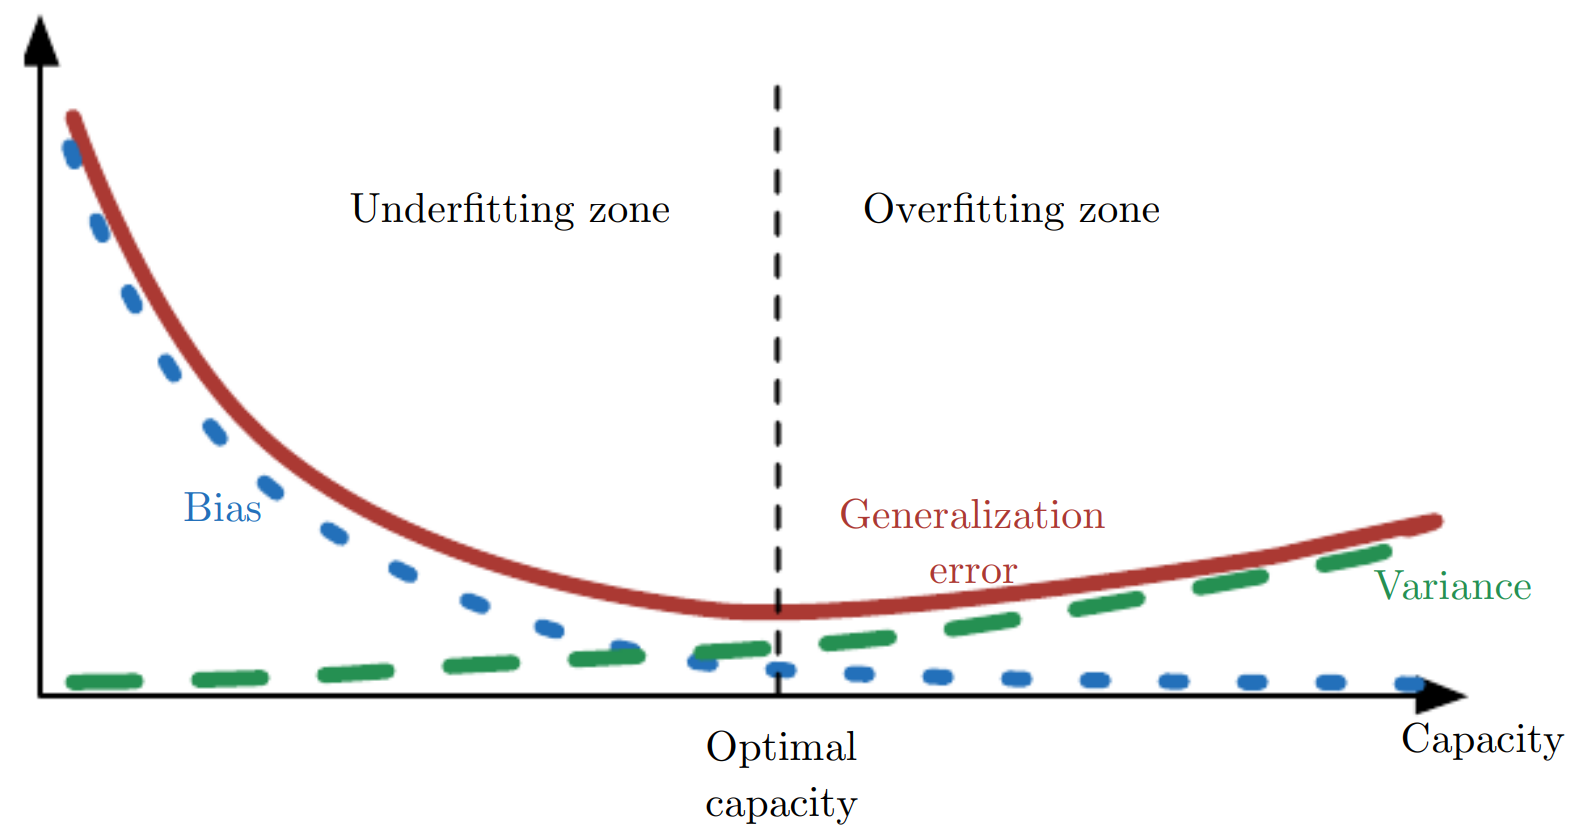
\includegraphics[scale=.4]{img/underoverfitting.png}
		\captionsetup{margin=2cm}
		\caption{Bias and Variance trade-off. As the capacity (complexity) of the model increases (x-axis), bias (dotted) tends to decrease and variance (dashed) tends to increase. The optimal capacity occurs when both bias and variance errors are minimized. From \cite{goodfellow2016deep}.}
		\label{fig:underoverfitting}
	\end{center}
\end{figure}
\noindent When overfitting occurs, it is possible to adopt regularization strategies with the specific aim to reduce the variance. Such techniques may vary according to the algorithms and the structure of the problem; to summarize, we only take into account regularization strategies for neural networks. \\
According to \cite{goodfellow2016deep}, we can refer to regularization as “any modification we make to a learning algorithm that is intended to reduce its generalization error but not its training error.”  \\
Typical examples of regularization techniques concern L1 and L2, which can be theoretically applied to any algorithm as they add parameter norm-based penalty to the objective function. \\
Another common strategy, especially in \gls{dsp} applications, is the so called "data augmentation". This is particularly suited when the dataset is small, as it allows the generation of additional and more diversified data points through certain transformations conducted upon original instances. Data augmentation is the easiest and cheapest way to increase the amount of training samples; however, the acquisition of new data, when possible, is preferable.  The correct transformation to apply highly dependent on the particular application. In Figure \ref{fig:data_aug} it is possible to see different ways of doing augmentation on images. \\
\begin{figure}[H]
	\begin{center}
		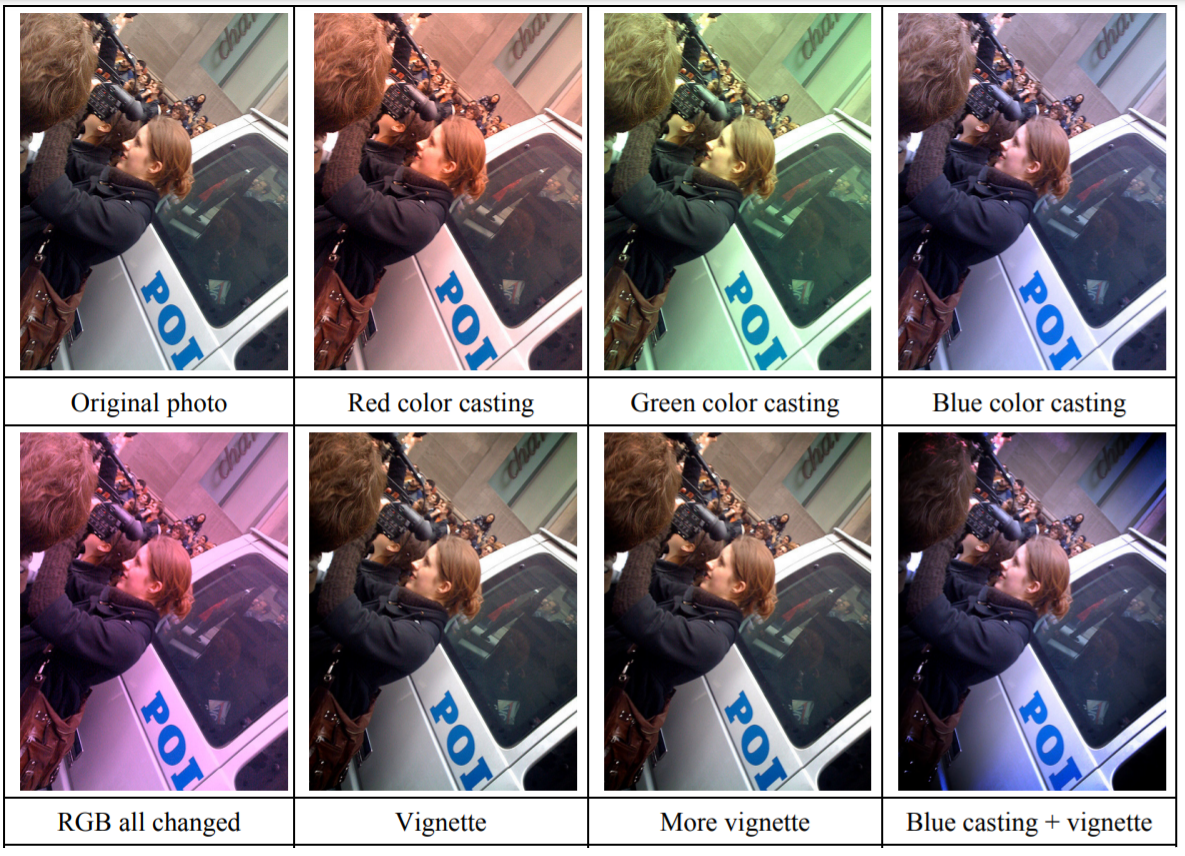
\includegraphics[scale=.55]{img/data_aug.png}
		\captionsetup{margin=2cm}
		\caption{Examples of color augmentations tested by Wu et al \cite{wu2015deep}.}
		\label{fig:data_aug}
	\end{center}
\end{figure}
\noindent Particularly worthy of mention are \textit{dropout}  \cite{srivastava2014dropout} and \textit{early stopping}, as they are two of the most used regularization strategies in \gls{dl} (and are both used in this project). \\
The former is a popular method to improve generalization by stochastically “dropping out” units during training to prevent their co-adaptation.\\
As for early stopping, briefly, it is based on choosing when to stop training a \gls{dl} model. The interruption criterion can vary wildly depending on the application; however, it is fair to say that it mostly depends on the loss on a validation set. An intuitive way of thinking about early stopping in \gls{dl} setting is to consider it as a hyperparameter selection method, where training time is the hyperparameter to be optimized.

\subsection{Convolutional Neural Networks} \label{cnns}
As previously motivated, \gls{cnn}s are an essential tool when facing \gls{dsp} problems and, for this reason, they are introduced in this section. \gls{cnn}s have revolutionized both the \gls{dsp} and the \gls{dl} fields, to the point that several \gls{dl}-based applications performs even better than human. \\ \gls{cnn} and, more generally \gls{dl}, came to mainstream popularity when Krizhevsky et al. \cite{krizhevsky2012imagenet} won the 2012 ImageNet Large-Scale Visual Recognition Challenge (ILSVRC \cite{ILSVRC15}) with a convolutional architecture called AlexNet. \\
The name Convolutional Neural Networks indicates that the system employs, in at least one of its layers, the convolution operation, which is previously introduced. Unlike in audio processing applications, where the convolution is generally applied only to one-dimensional signals, in \gls{dl} systems, usually this operation takes place between tensors, i.e. multidimensional vectors. Furthermore, in many \gls{dl} architectures the operation used in a \gls{cnn} does not correspond precisely to the traditional convolution: indeed, there are several variants such as the one defined in paragraph \ref{dilated_conv}. \\
\begin{figure}[H]
	\begin{center}
		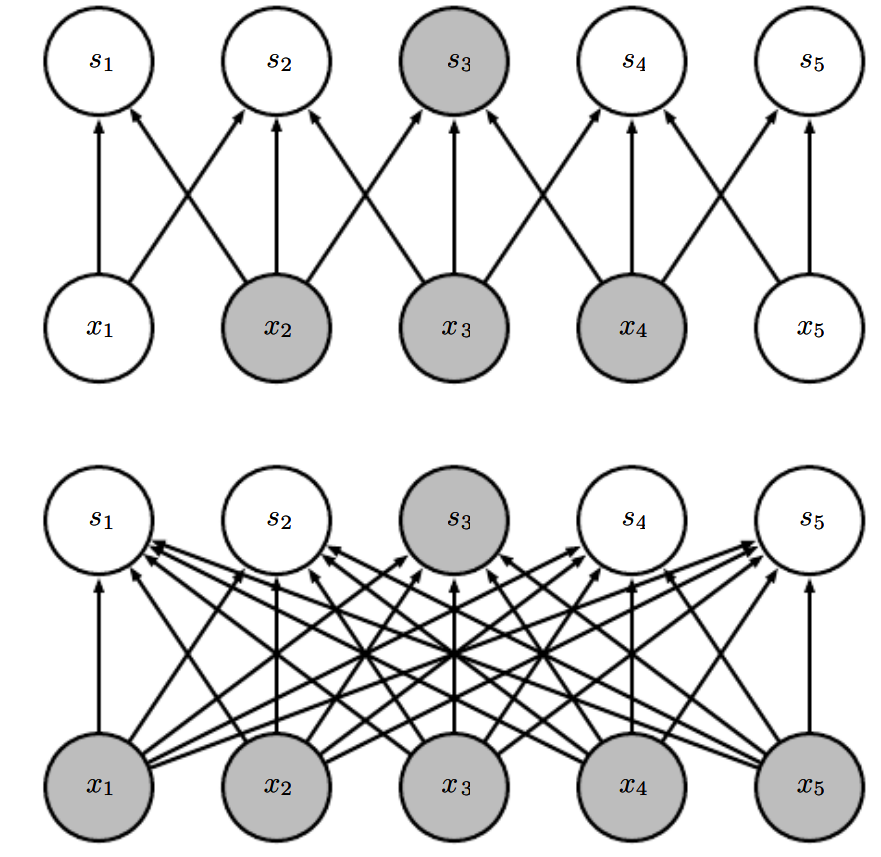
\includegraphics[scale=.5]{img/sparse_interactions.png}
		\captionsetup{margin=2cm}
		\caption{Graphical representation of the connections between input and output units in both convolutional and fully connected approaches. \textit{Top:} When we use \gls{cnn} layers with a kernel of width 3, the connectivity is sparse such that each output unit is affected only by 3 input units. \textit{Bottom:} In fully connected layers each output unit is formed by matrix multiplication, so that all of the inputs affect the highlighted $s_3$.
			From \cite{goodfellow2016deep}.}
		\label{fig:sparse_interactions}
	\end{center}
\end{figure}
\noindent One of the main advantages of \gls{cnn}s over traditional fully connected layers is that they allows to reduce the memory requirements by limiting the number of connections between input and output units. Thus, while in fully-connected layers forward propagation as well as backpropagation are expressed as matrix multiplications, \gls{cnn} layers use convolution which connects input and output units sparsely. This \textit{sparse connectivity} (also referred to as \textit{sparse interactions}) in convolutional networks reduces the computational complexity since the output computation requires fewer operations. In particular, the higher the \textit{receptive filed} of a convolutional layer is, the higher is the number of parameters, i.e. the memory requirements. A graphical illustration of the sparse interactions between input and output units is given in Figure \ref{fig:sparse_interactions}. \\
Even if direct connections in a convolutional net are very sparse, units in the higher layers can indirectly interact with a larger portion of the input. In other words, deeper layers receive generally more global information since the receptive field of the units in the higher layers is larger than the one of the units in the shallow layers. Furthermore, this effect is more pronounced if the system includes operations like \textit{pooling} (see the book \cite{goodfellow2016deep}). A graphical example of this intuitive concept is given in Figure \ref{fig:deeperlayers}. \\
\begin{figure}[H]
	\begin{center}
		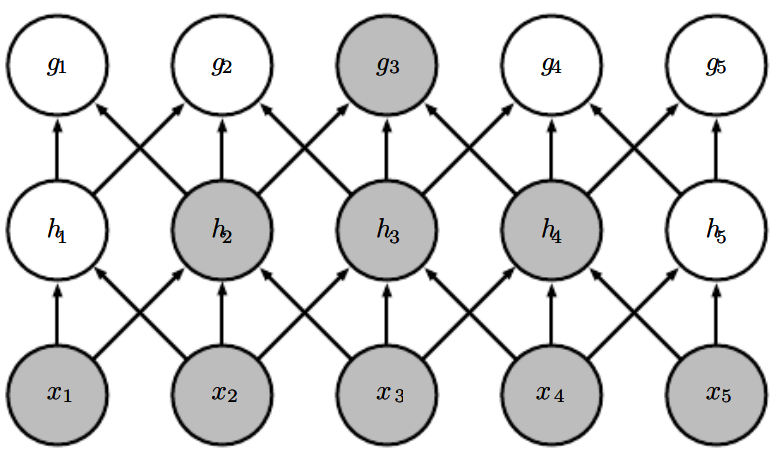
\includegraphics[scale=.5]{img/deeperlayers.png}
		\captionsetup{margin=2cm}
		\caption{Deeper layers can indirectly interact with a larger portion of the input.
From \cite{goodfellow2016deep}.}
		\label{fig:deeperlayers}
	\end{center}
\end{figure}
\noindent As previously motivated, deep convolutional networks are particularly suitable to capture complicated non-linear interactions between data points. The learning process leads to the creation of deep latent variables, which are quite difficult for a human to interpret. Because of this “black-box” nature, \gls{dl} models suffer from providing meaningful interpretations of their results. For this reason, the interpretation of deep networks is a very active research area, and many works in literature aims to discover what a \gls{cnn} really learns from data.\\
An interesting paper is that of Zeiler and Fergus \cite{zeiler2014visualizing} who works on images. They demonstrate that different layers of a \gls{cnn} respond distinctively to specific aspects of images. In particular, they discover that early hidden layers detect low-level features such as edges, corners and shapes, while deeper layers extract more abstract (high-level) information, such as categories or objects. Figure \ref{fig:cnnviz} provides a graphical example of this information hierarchy during the \gls{cnn} learning process.\\
\begin{figure}[H]
	\begin{center}
		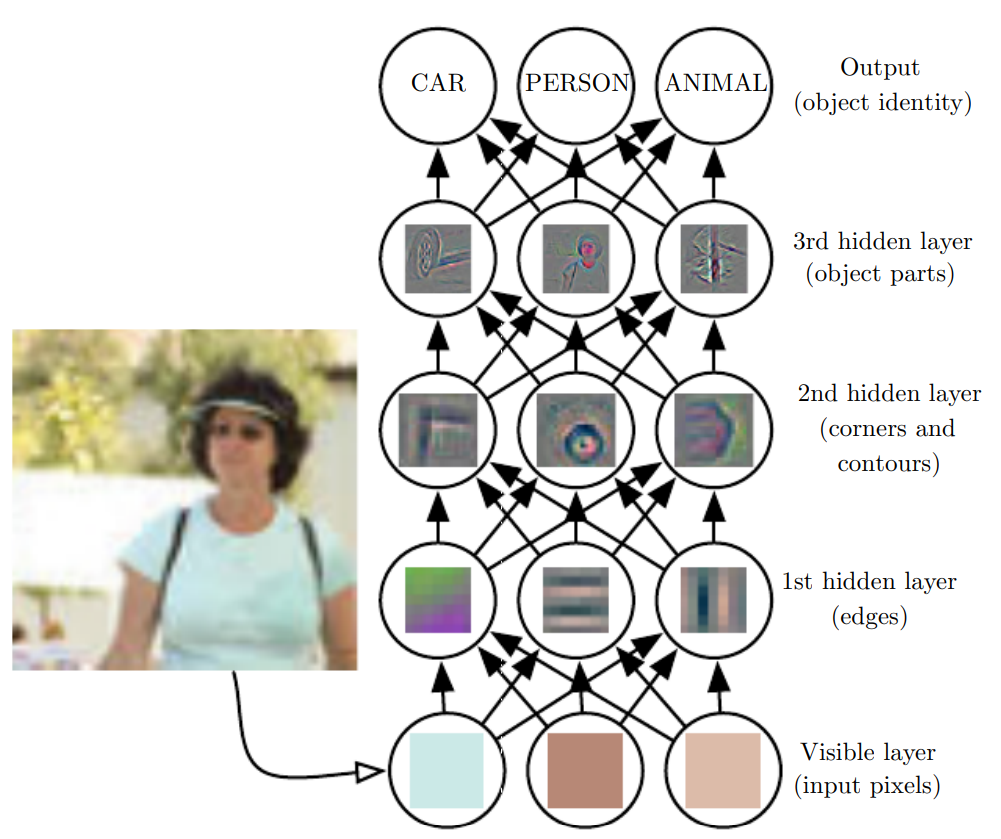
\includegraphics[scale=.7]{img/cnnviz.png}
		\captionsetup{margin=2cm}
		\caption{A convolutional neural network extracts increasingly abstract
			features from an image. From \cite{goodfellow2016deep}.}
		\label{fig:cnnviz}
	\end{center}
\end{figure}
\subsection{Recurrent Neural Networks}
In a traditional neural network we assume that input and output data do not follow a specific order; in other words, the implicit assumption is that data points are independent of each other. Although this assumption is valid in many problem settings, it is extremely limiting in others. For example, if we want to analyze historical data representing the global earth temperature, we have to take into account the implicit time axis between each observation. In speech processing too, data points are dependent of each other and this leads to the need for an appropriate sequential modelling. \\
Recurrent neural network approaches arise from this need: according to \cite{goodfellow2016deep}, much as a \gls{cnn} is particularly suited for processing data that have a grid pattern, such as images, a \gls{rnn} is specialized for processing time series, or, more generally, sequential data. An intuitive way to think about \gls{rnn}s is that they have a sort of "memory" which stores relevant information about what they have processed so far. \\
More specifically, \gls{rnn}s define recurrence relations between data points by introducing cycles in their computational graph to efficiently model this sequential influence. \\
The basic idea behind recurrent approaches is that, at each time step, an interaction takes place through hidden recurrent connections. This interaction, which involves a cycle in the graph computation, is graphically represented by a black square in Figure \ref{fig:rnn_graph}. \\
\begin{figure}[H]
	\begin{center}
		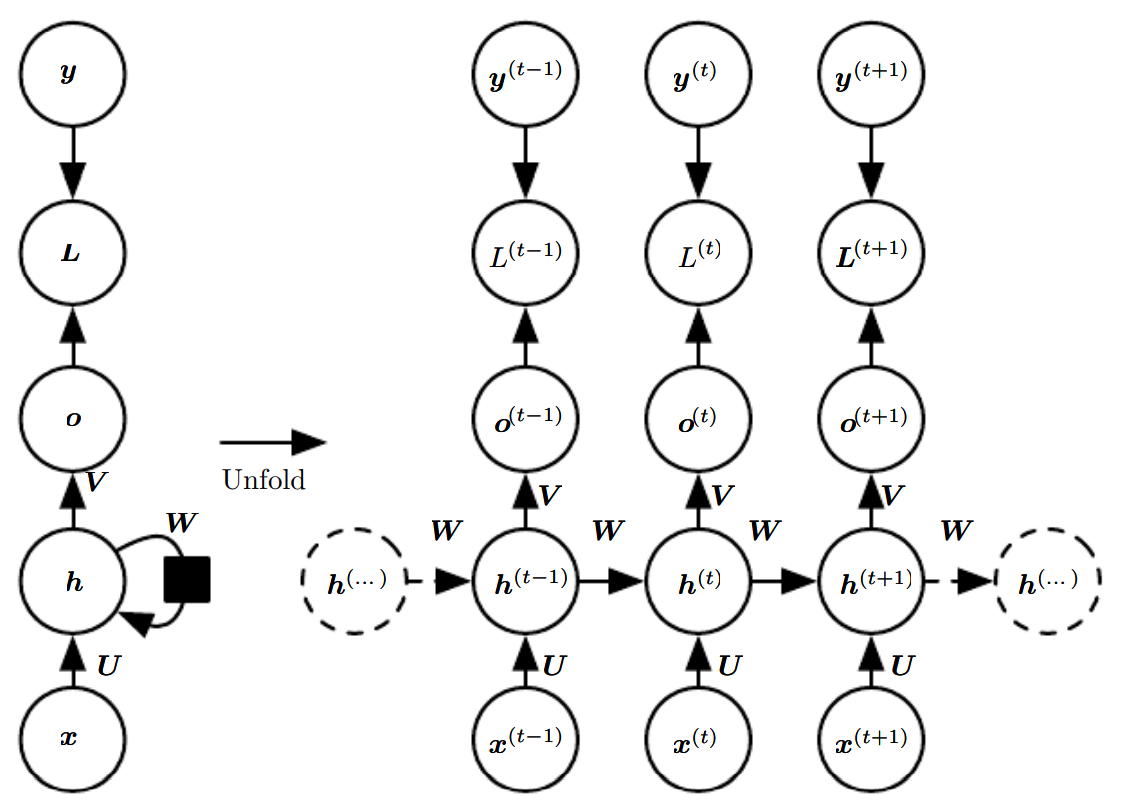
\includegraphics[scale=.58]{img/rnn_graph.png}
		\captionsetup{margin=2cm}
		\caption{"The computational graph to compute the training loss of a recurrent network that maps an input sequence of \textbf{x} values to a corresponding sequence of output \textbf{o} values.	A loss \textbf{L} measures how far each \textbf{o} is from the corresponding training target \textbf{y}. When using softmax outputs, we assume \textbf{o} is the unnormalized log probabilities. The loss \textbf{L} internally computes \textbf{$\hat{y}$} = softmax(\textbf{o}) and compares this to the target \textbf{y}. The \gls{rnn} has input to hidden connections parametrized by a weight matrix \textbf{U}, hidden-to-hidden recurrent connections parametrized by a weight matrix \textbf{W}, and hidden-to-output connections parametrized by a weight matrix \textbf{V}". \textit{Left:} Circuit diagram representation. \textit{Right:} The same \gls{rnn} seen as an unfolded computational graph. From \cite{goodfellow2016deep}.}
		\label{fig:rnn_graph}
	\end{center}
\end{figure}
\noindent Figure \ref{fig:rnn_graph} illustrates a simple \gls{rnn} that processes the information from the input \textbf{x} by incorporating it into the state \textbf{h} that is passed forward through time. \\
It is noticeable that this architecture aims to produce an output at each time step and has recurrent connections between hidden units. Although this is a common schema, it may not be the rule. Indeed, depending on the task, it might be reasonable to adopt other architectural configurations. For example, when working on a speaker identification task, we aim to obtain the final output after the whole input recording is processed, not after each audio sample. In this case we need a \gls{rnn} that reads an entire sequence and produces a single output, such as the one illustrated in Figure \ref{fig:rnn_single_output}. \\
\begin{figure}[H]
	\begin{center}
		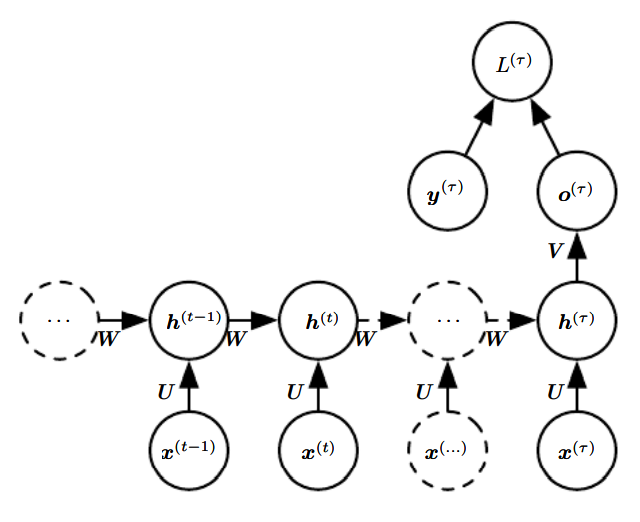
\includegraphics[scale=.75]{img/rnn_single_output.png}
		\captionsetup{margin=2cm}
		\caption{Time-unfolded \gls{rnn} with a single output at the end of the sequence. From \cite{goodfellow2016deep}.}
		\label{fig:rnn_single_output}
	\end{center}
\end{figure}
\noindent It is important to mention that recurrent networks are trained through the Backpropagation Through Time algorithm (\cite{rumelhart1985learning}, \cite{werbos1990backpropagation}), which computes the gradient of model error with respect to its weights. \\
Common problems in recurrent \gls{dl} approaches are the ones of \textit{vanishing} and \textit{exploding} gradients. Especially traditional \gls{rnn}s suffer from it: if the gradient tends to be very close to zero in the training process, the network weight correction vanishes and, consequently, the backpropagation through time fails. \\
One possible solution to reduce the effect of vanishing gradients would be to adopt \textit{gated} \gls{rnn}s architectures. These special sequence models include \gls{lstm}\cite{hochreiter1997long} and \gls{gru}\cite{chung2014empirical}. Without going into too much detail, gated \gls{rnn}s are based on the idea of creating few trainable gates (paths) to select the most important information to memorize through time. These pieces of informations are then propagated by connection weights that may change at every time step. For a more formal and comprehensive description of these recurrent approaches we encourage to consider deep learning textbooks, such as \cite{goodfellow2016deep}.  %read tex file from chapters folder 

\chapter{Methods for Artificial Bandwidth Extension} \label{chap:methods}
As said in Chapter 1, the proposed strategy to solve the audio \gls{sr} task is based on an hybrid architecture that combines both \gls{tfnet} \cite{lim2018time} and \gls{tfilm} \cite{birnbaum2019temporal} methods. In order to describe our system, a previous analysis of the two models from which the proposed one derives needs to be done. For this reason, both \gls{tfnet} and \gls{tfilm} approaches are described in paragraphs \ref{tfnet} and \ref{tfilm}, respectively. \\
All methods for audio \gls{sr} that are presented in this chapter derive from a mathematical formulation that treats this task as a pure regression problem.
As stated in paragraph \ref{problem_formulation}, the goal of the model is to characterize the conditional distribution $p(y|x)$ of a \gls{hr} sequence given its \gls{lr} input. Therefore, the point-estimate output results in a sequence $\hat{y} = f_{\theta}(x)$ of real values. This formulation naturally leads to the least-squares optimization problem of the form:
\begin{align}\label{eq:regression_formulation}
	\begin{array}{c}
		\min _{\theta} \sum_{i}\left\|f_{\theta}(x_{i})-y_{i}\right\|_{2}^{2}
	\end{array}
\end{align}
where $\|.\|$ denotes the norm function, $x_i, y_i$ are training examples such that $\mathcal{D} = \{x_i, y_i\}_{i = 1}^n$ and $f_{\theta}$ is the \gls{dl} model parametrized by $\theta$. As a natural consequence of this setting, the objective function of this work can be defined as:
\begin{align}\label{eq:regression_loss}
	\begin{array}{c}
		\ell(\mathcal{D})=\frac{1}{n} \sqrt{\sum_{i=1}^{n}\left\|y_{i}-f_{\theta}\left(x_{i}\right)\right\|_{2}^{2}}
	\end{array}
\end{align}
In other words, artificial \gls{bwe} can be seen as a structured regression task, where the goal is to minimize the difference between the model point estimation and the target sequence. \\
The problem can be tackled by deep neural network architectures, that have enough capacity to perform non-linear regression. Indeed, many levels of non-linearities allow them to represent a complex non-linear regression function that maps \gls{lr} input data to \gls{hr} audio frames. Therefore, all \gls{dl} systems presented in this chapter are trained in order to minimize the metric given in Equation \ref{eq:regression_loss}. \\
Another common factor shared by all of these audio \gls{sr} methods is that the source input is pre-processed with a  a cubic B-spline upscaling in order to ensure \gls{lr}/\gls{hr} signals are of the same length. This operation has multiple advantages. On one hand, it allows to have a baseline to compare the results of \gls{dl} models. On the other hand, since this operation is included in the processing pipeline, it is possible to exploit it by the use of residual connections to link the input and the output series. This solution allows to speed up the required training time, because the model  $f_{\theta}$ is facilitated by having to estimate only the difference between the \gls{lr} source and the target \gls{hr} signal. This and all other pre-processing operations are discussed in detail in Chapter ~\ref{chap:exp_results}. \\
It is important to point out that, due to computational limitations, it is not possible, in this work, to propose and train a new model that has the same number of parameters than \gls{tfnet} and \gls{tfilm}. Therefore, results reported in the two model papers can not be used to make comparisons between different architectures. In fact, model comparisons must be performed in fair contexts, i.e., by training models with approximately the same number of parameters. For this reason, \gls{tfnet} and \gls{tfilm} models are
reduced in size and, subsequently, re-trained so that they can be compared with the proposed architecture under the same conditions. \\
This chapter aims not only to provide a clear idea of the original configurations of the models, but also to describe the changes made to reduce dimensionality. Therefore, in the paragraphs \ref{tfnet} and \ref{tfilm}, the models \gls{tfnet} e \gls{tfilm}, respectively, are described in their original configurations. Then, in the paragraph \ref{implementation_details}, all
details related to the implementation of the models, and the changes made to the original configurations are thoroughly described.

\section{TFNet} \label{tfnet}
Time-Frequency Network, proposed by Lim, Yeh \textit{et  al.}\cite{lim2018time}, is the first model in literature that addresses the problem of audio \gls{sr} by operating in both time and frequency domain. In the paper, authors highlight the origin of their intuition. “At the first glance, modeling in both frequency and time domain seems like a redundant representation; From Parseval’s theorem the $\ell_{2}$ difference of prediction error, whether in the frequency or time domain is exactly the same. However, regression from \gls{lr} to \gls{hr} in time or frequency domain solves a very different problem. In the time domain, it is analogous to the image super-resolution task, mapping \textit{audio patches} from \gls{lr} to \gls{hr}. On the other hand, \gls{sr} in the frequency domain is analogous to the \textit{semantic image inpainting} task (\gls{bwe} in spectral domain can be viewed as image inpainting of spectrograms) \cite{pathak2016context},\cite{yeh2017semantic}”. \\
\begin{figure}[H]
	\begin{center}
		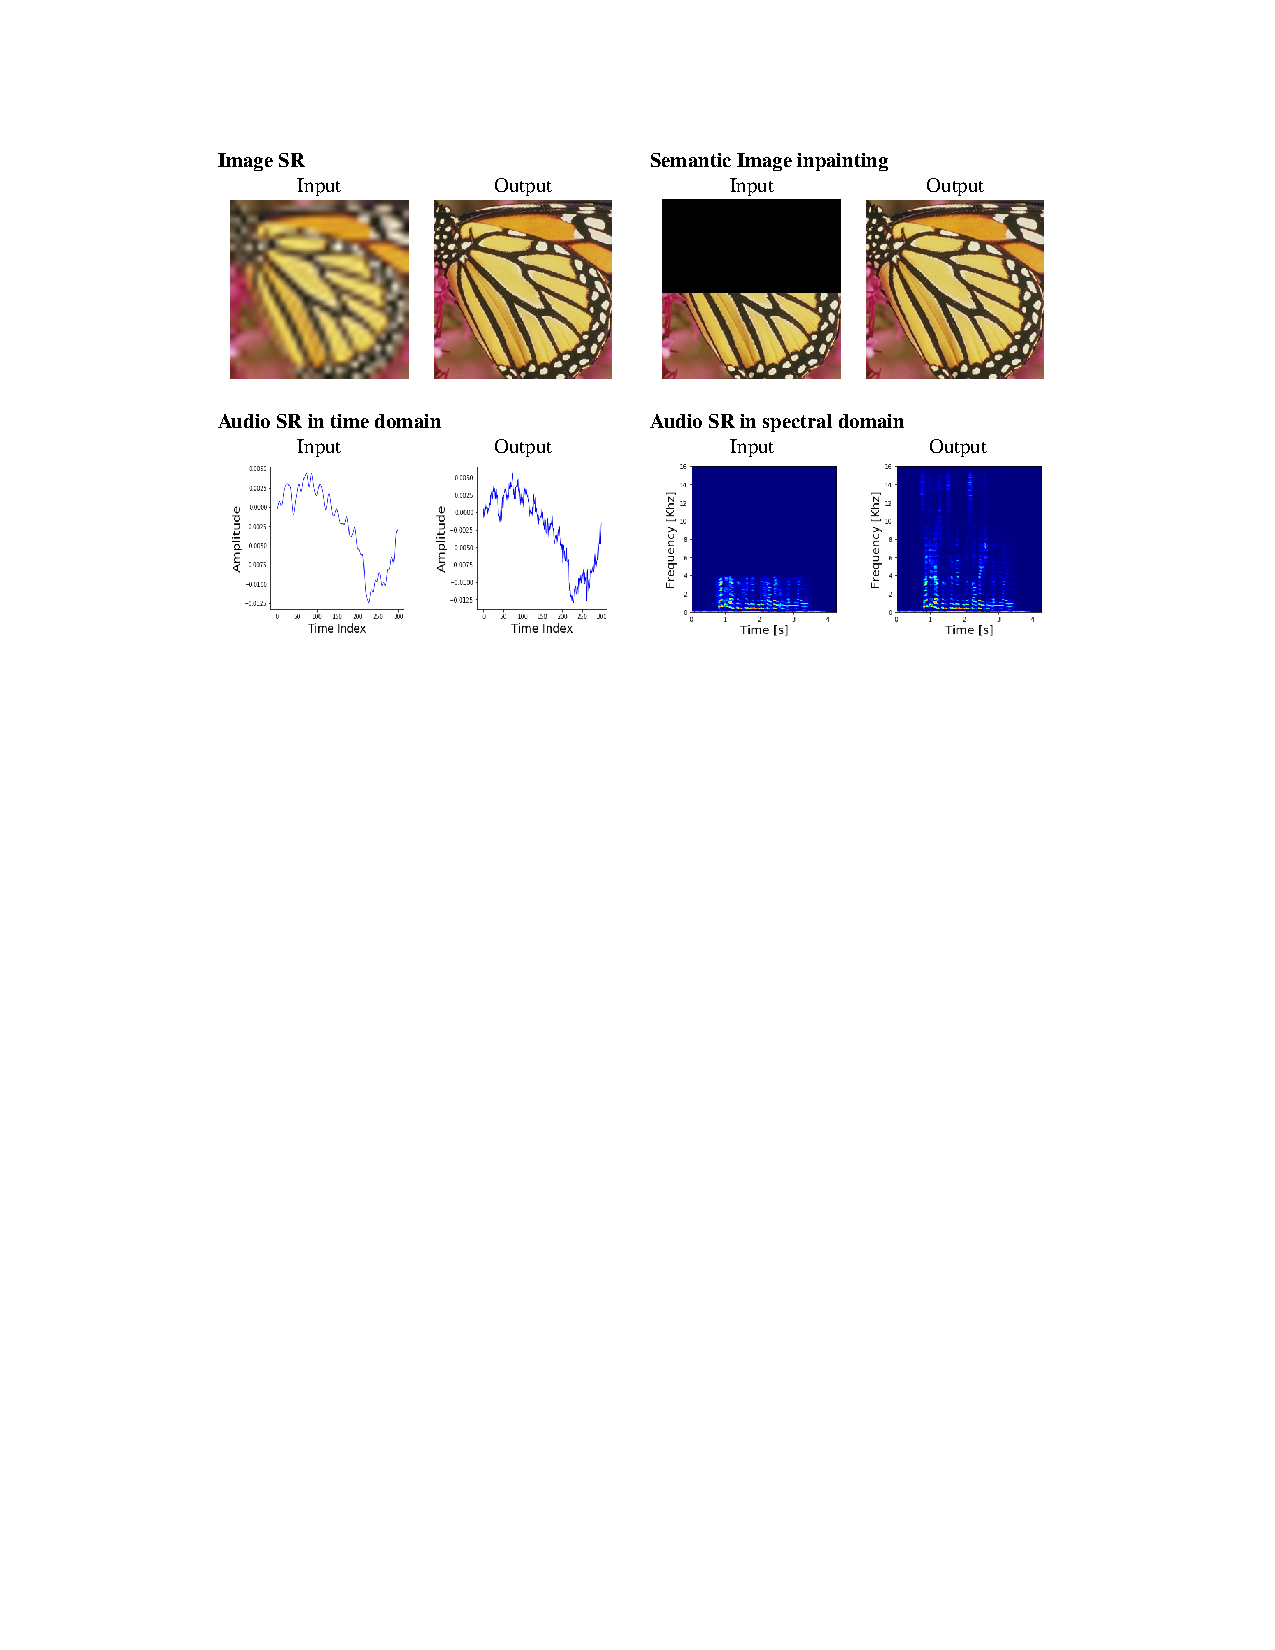
\includegraphics[scale=1.11]{img/tfnet_intuition.pdf}
		\captionsetup{margin=2cm}
		\caption{\textit{Top row}: Examples of image \gls{sr} and semantic image inpainting reconstruction. \textit{Bottom row}: Illustration of the input/output for audio \gls{sr} in time and frequency domain. From \cite{lim2018time}.}
		\label{fig:tfnet_intuition}
	\end{center}
\end{figure}
\noindent Figure ~\ref{fig:tfnet_intuition} sums up the close relationship that links audio \gls{sr} in time domain with image \gls{sr}, and audio \gls{sr} in frequency domain with image inpainting. \\
Based on these considerations, authors propose a system made of two main branches: one which models signals in the spectral domain, while the other branch explicitly models the reconstruction in time domain. \\
More specifically, \gls{tfnet} is a fully differentiable network that estimates, for a given \gls{lr} input $x$, the \gls{hr} audio reconstruction $\hat{z}$, and the \gls{hr} spectral magnitude $\hat{m}$. The last layer of the model, called \textit{Spectral Fusion Layer}, computes Fourier transform operations in order to combine $\hat{z}$ and $\hat{m}$ in a unique output $\hat{y}$. \\
A brief overview of the overall pipeline of the model architecture is provided in Fig. ~\ref{fig:tfnet_pipeline}. As we can see, the time-domain branch processes the signal through the "Slim AudioUNet" that is a fully convolutional component, explained in detail in \ref{audiounet}. The frequency branch performs more operations during the system processing: first, a \gls{dft} on the sequence is computed to pass from one domain to another. It is well known that when the \gls{dft} is performed on purely real input, such as audio signals, negative phase components are redundant and can be discarded. This is because the \gls{dft} of a real signal is Hermitian-symmetric, i.e. negative-frequency terms can be obtained from the corresponding positive terms. Therefore, given the \gls{lr} input signal $x$ of length $T_1$, only $\frac{T_1}{2} + 1$ components are taken into account: the zero-frequency term (DC component) followed by the $\frac{T_1}{2}$ positive-frequency terms. These $\frac{T_1}{2}$ values are then processed through the "Spectral Replicator" and "Slim AudioUNet", while the zero-frequency term pass directly through the network. A final concatenation operation is  applied in order to combine the DC component with the processed positive-frequency terms. \\
All the details concerning architectural components not yet presented, such as "Slim AudioUNet", "Spectral Replicator" and "Spectral Fusion Layer", are thoroughly studied in the next paragraphs. 

\begin{figure}[!htb]
	\begin{center}
		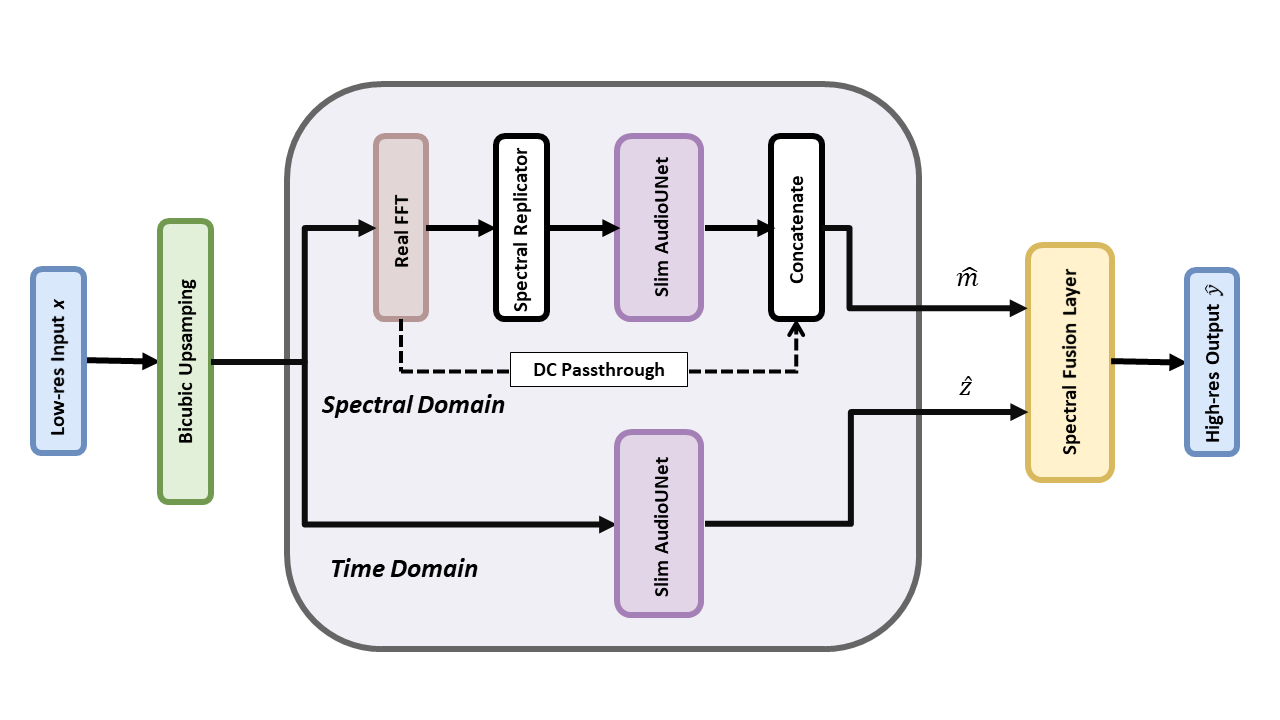
\includegraphics[scale=0.48]{img/tfnet_pipeline.png}
		\captionsetup{margin=2cm}
		\caption{Overall pipeline of \gls{tfnet}. The system exploits both time and frequency domain information in order to map the \gls{lr} input $x$ to the \gls{hr} reconstruction $\hat{y}$. From \cite{lim2018time}.}
		\label{fig:tfnet_pipeline}
	\end{center}
\end{figure}

\subsection{AudioUNet} \label{audiounet}
AudioUNet is a fully feedforward network that consists of downsampling and upsampling blocks. The model was originally designed by Kuleshov \textit{et al.} \cite{kuleshov2017audio}, who demonstrates the effectiveness of convolutional architectures on the \gls{bwe} task. \\
As Figure ~\ref{fig:audiounet} shows, the model has a bottleneck architecture, that is designed in order to encourage the model to learn a hierarchy of features, such as auto-encoders. In this regard, it is possible to reasonably imagine that, on an audio task, bottom layers may learn wavelet-like patterns, while top ones may correspond to more complex audio units, such as phonemes \cite{aytar2016soundnet}.\\
AudioUNet is a fully convolutional neural network with residual connections. It contains $B$ successive encoder/decoder blocks that produce dimensionally mirrored outputs: downsampling components halve the temporal (or spatial) dimension and double the number of filters, while upsampling components do the opposite. \\
Moreover, each block performs a specific series of operations. In particular, encoder blocks perform only Convolution and Leaky \gls{relu}, while the bottleneck layer and decoder components perform Dropout too. \\
It is important to mention that, during the upsampling stage, two more operations for the improvement are conducted: one-dimensional Subpixel shuffling and residual connections concatenation. The former consists in a principled reshape of tensors. It was originally designed to work on two-dimensional signals: \textit{Shi et al.} demonstrate that this operation produce less artifacts on images reconstructed by a \gls{sr} algorithm \cite{shi2016real}. Authors of AudioUNet reasonably assume that this property can be extended to audio signals as well. As for residual connections, their use is motivated by the fact that, in a bottleneck architecture, when the input is similar to the target, downsampling features can be also useful for upsampling \cite{zhang2016colorful}. These two operations are linked by the following pipeline: the subpixel layer reshuffles a tensor $F \in \mathbf{R}^{T \times C}$ (where $T$ is the temporal dimension, while $C$ is the number of channels), into another one of size $F \in \mathbf{R}^{\frac{T}{2} \times2C}$; these are concatenated, through a skip connection, with $\frac{T}{2}$ features from the downsampling stage, for a final output of size $F \in \mathbf{R}^{T \times2C}$. Finally, a further skip connection is used to link the input data and the final reconstruction.
\begin{figure}[!htb]
	\begin{center}
		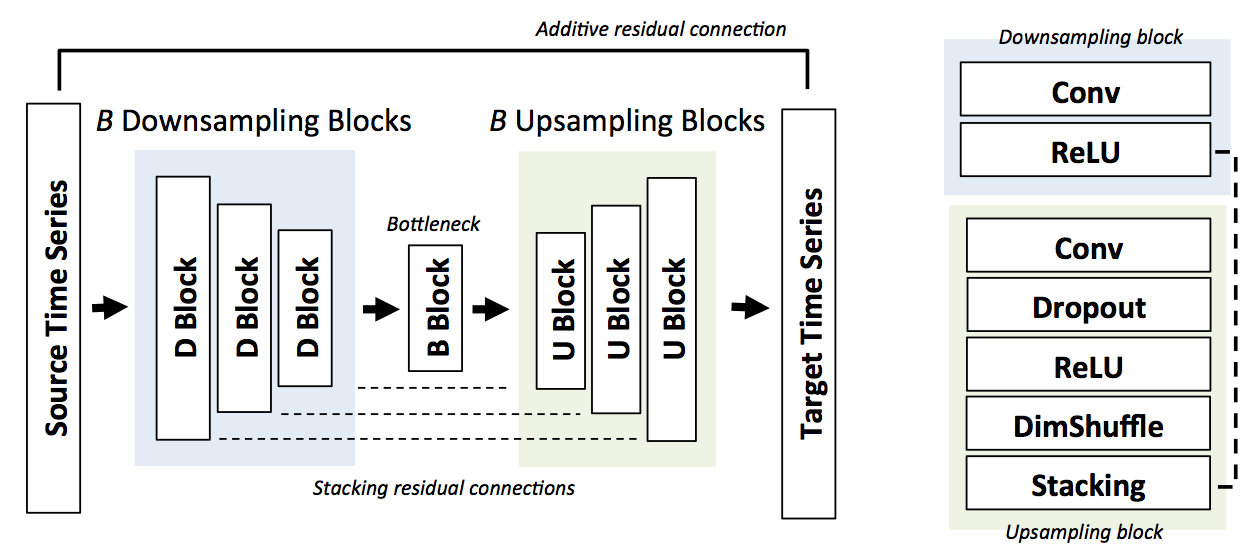
\includegraphics[scale=0.35]{img/audiounet.png}
		\captionsetup{margin=2cm}
		\caption{AudioUNet architecture. It consists of B successive downsampling/upsampling blocks linked by residual connections. From \cite{kuleshov2017audio}.}
		\label{fig:audiounet}
	\end{center}
\end{figure}
\noindent Figure ~\ref{fig:tfnet_pipeline} clearly illustrates that AudioUNet is used to model both the audio reconstruction and the spectral magnitude. It is important to indicate that B (the number of upsampling and downsampling blocks) is equal to 4 in both time and spectral branches. \\
As for the terminology used by Lim, Yeh \textit{et al.}, the term “Slim AudioUNet” in Fig. ~\ref{fig:tfnet_pipeline} refers to the fact that they reduce the original dimension of the network by halving the number of filters in each of the branch. Otherwise, the model is equal to the one just described.

\subsection{Spectral Replicator} \label{spectral_replicator}
As mentioned previously, the problem of audio \gls{sr} is based on the hypothesis that it is possible to reconstruct the high-frequency content of a signal from its corresponding low-frequency counterpart. The Spectral Replicator is a layer designed in order to alter the content of an input spectrum such that this low-high frequency dependency is explicitly expressed. The idea behind the design of this component is described in detail below. \\
Given that the objective of the system is to increase the sampling rate of a signal, it must be taken into account that, due to the Nyquist limit, there are some frequency components in the \gls{hr} target that can not exist in the \gls{lr} input sequence. It is possible to explain this concept formally in the following way. \\
Recalling the notation introduced in paragraph \ref{problem_formulation}, suppose we are trying to increase the temporal resolution of a signal $x$ sampled at $R_1$ by a factor of $r$. From the \gls{dsp} theory, we know that the Nyquist rate for that signal is equal to $R_{1_{lim}} = \frac{R_1}{2}$. However, the theoretical limit frequency of the \gls{hr} sequence is equal to $R_{2_{lim}} = r \times R_1$. From this point of view, audio \gls{sr} problem can be seen as the task of estimating the missing frequency components between $R_{1_{lim}}$ and $R_{2_{lim}}$. In other words, the aim of the system is to reconstruct the values over the interval $\interval{R_{1_{lim}}}{R_{2_{lim}}}$, on which the spectrum of the \gls{lr} sequence is null. \\
As mentioned extensively in the previous section, the reconstruction is made by a convolutional approach. Here arises a problem, since convolution is a local operation, i.e. only short-range dependencies in sequential inputs can be captured and processed due to the receptive field limitation. In other words, convolution cannot fully investigate non-local joint dependencies that could be useful to estimate the \gls{hr} spectrum. Therefore, it can be too challenging for a fully convolutional model to make the output’s high frequency component depend on the input’s low frequency counterpart. This limitation is accentuated as the scaling ratio $r$ increases, because the interval $\interval{R_{1_{lim}}}{R_{2_{lim}}}$ gets larger. \\
To overcome this issue, the Spectral Replicator layer explicitly replicates $r - 1$ times the low-frequency part of the signal, compensating the limitations of convolutional approaches. Therefore, all the zeros in the high frequency components of the spectrum are replaced by copies of the low frequency respective counterpart.\\
Specifically, each frequency term $k_i \in \interval{k_1}{k_{\frac{T_1}{2}}}$ (where $T_1$ is the length of $x$) is copied $r$ times through this layer. The only exception is given by the term $k_0$ (DC component), that, as said before, is not processed through the Spectral Replicator. \\
For example, suppose to have a signal $x$ whose spectral content is limited by the frequency term $k_{1024}$. For $4\times$ upsampling, we replace the zeros over the interval $\interval{k_{1025}}{k_{4096}}$ by repeating the 1st component to the 1024th one at 1025 to 2048, 2049 to 3072 and finally 3073 to 4096. Finally, these 4096 values are concatenated with the $k_0$ term. \\
Figure ~\ref{fig:spectral_replicator} illustrates the Spectral Replicator layer working on the \gls{bwe} task with $r = 4$. The input signal $x$ in the example has a sampling frequency of $R_1 =$ 8kHz, so that the Nyquist limit is $R_{1_{lim}} =$ 4kHz. As we can see, the low frequency patterns are replicated multiple times such that the zeros are replaced. \\
\begin{figure}[!htb]
	\begin{center}
		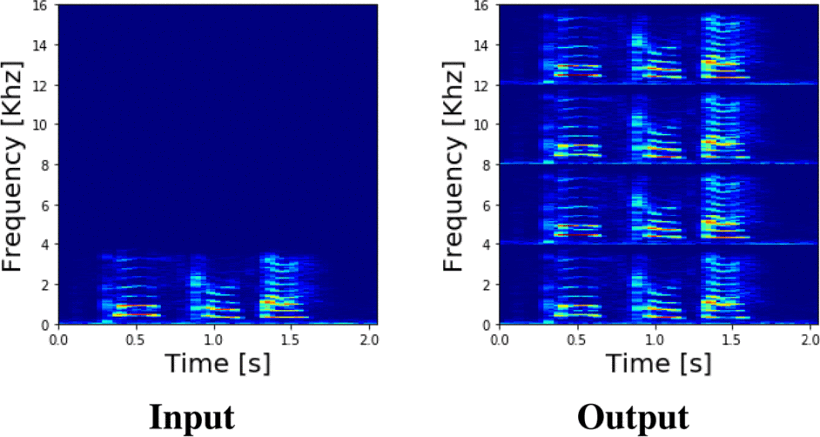
\includegraphics[scale=0.65]{img/spectral_replicator.png}
		\captionsetup{margin=2cm}
		\caption{Spectrogram showing how the signal is processed through the Spectral Replicator layer. The low-frequency components of the input spectrum are replicated three times in order to replace zeros in the high-frequency counterpart. From \cite{lim2018time}.}
		\label{fig:spectral_replicator}
	\end{center}
\end{figure} 
\subsection{Spectral Fusion Layer}
The spectral Fusion Layer is a key component of the \gls{tfnet} architecture. It permits to combine outputs of the two branches, i.e. $\hat{m}$ and $\hat{z}$, in a single \gls{hr} final reconstruction. To recap, the model predicts, for a given \gls{lr} input $x$, the estimation of the \gls{hr} audio reconstruction $\hat{z}$, and the \gls{hr} spectral magnitude $\hat{m}$. These two quantities are finally synthesized in the temporal domain through this layer. \\
Specifically, the process through which this happens consists of two main stages. First of all, since the two branches operate in two different domains, there is the need to reduce the data to the same domain. This operation is performed according to the following equation, which defines the \gls{hr} spectral magnitude estimate. 
\begin{align}\label{eq:spectralfusion1}
	\begin{array}{c}
		M=w \odot|\mathscr{F}(\hat{z})|+(1-w) \odot \hat{m}
	\end{array}
\end{align}
Equation ~\ref{eq:spectralfusion1} shows that the final estimation of the \gls{hr} spectral magnitude is a weighted average of the individual estimates provided by each branch. A data-driven approach is used to establish the weight of each branch in this operation. Indeed, this equation involves an element-wise multiplication with the trainable parameter $w$. \\
The second stage consists in calculating the final output $\hat{y}$ through Equation ~\ref{eq:spectralfusion2}. This one, is used to bring back the data to the original domain, i.e. the temporal one. Moreover, this second equation shows that the \gls{hr} phase is estimated only in the time domain.
\begin{align}\label{eq:spectralfusion2}
	\begin{array}{c}
		\hat{y}=\mathscr{F}^{-1}\left(M e^{j \angle \mathscr{F}(\hat{z})}\right)
	\end{array}
\end{align}
The Spectral Fusion Layer is fully differentiable and can be trained end-to-end.

\section{TFiLM} \label{tfilm}
The main objective of this paragraph is to present Temporal Feature-Wise Linear Modulation, a neural network component proposed by Birnbaum, Kuleshov \textit{et al.} in 2019 \cite{birnbaum2019temporal}. The key contribution of their work is to show that it is possible to capture long-term information in sequential inputs by combining elements of convolutional and recurrent approaches. \\
The main intuition behind the \gls{tfilm} approach is as follows. \gls{cnn}s, which are extensively used for audio \gls{sr}, can effectively process digital signals, such as audio, images or video and are relatively easy to train. However, these models have some disadvantages that could limit their prediction performance. In particular, convolutional approaches are not well suited for long sequential data processing because of the limited receptive field, which results in insufficient capacity to capture long-range input dependencies. Indeed, the larger the receptive field, the more a convolutional model is computationally complex. To overcome this issue, the researchers propose a particular architectural component that can capture both short and long-term interactions between features.\\
In summary, the \gls{tfilm} algorithm can be viewed as a temporal adaptive normalization layer that modulates the activations of a convolutional layer through a \gls{rnn}. More specifically, this algorithm takes as input a tensor of 1D multichannel convolutional activations $F \in \mathbf{R}^{T \times C}$ where $T, C$ are, respectively, the temporal dimension and the number of channels, and a positive integer value $B \in \mathbf{N}^{+}$ that identifies the block length. The output is an adaptively normalized tensor of activations $F' \in \mathbf{R}^{T \times C}$. The whole algorithm pipeline can be divided into five steps:
\begin{enumerate}
	\item Reshape $F$, along the spatial dimension, into a block tensor $F^{\mathrm{blk}} \in \mathbf{R}^{B \times T / B \times C},$ defined as $F_{b, t, c}^{\mathrm{blk}}=F_{b \times B+t, c}$. Each block can be considered as a region along the time axis in which the audio samples are closely correlated; for example, when processing audio, blocks could reasonably correspond to a set of activations that define a possible phoneme. 
	\item Obtain a representation $F^{\text {pool }} \in \mathbf{R}^{B \times C}$ of the block tensor by pooling together the channels within each block: $F_{b, c}^{\mathrm{pool}}=\operatorname{Pool}\left(F_{b,:, c}^{\mathrm{blk}}\right)$.
	\item  Compute, for $b=1,2, \ldots, B$, an affine transformation $\left(\gamma_{b}, \beta_{b}\right), h_{b}=\operatorname{RNN}\left(F_{b, \cdot}^{\text {pool }} ; h_{b-1}\right)$ using an \gls{rnn} applied to pooled blocks. The first value is $h_{0}=\overrightarrow{0}$, where $h_b$ denotes the hidden state and $\left(\gamma_{b}, \beta_{b}\right)$ is a tuple of trainable parameters. 
	\item Activations in each block b are normalized by $\gamma_{b}, \beta_{b}$. Formally, normalized block tensor $F^{\text {norm }} \in \mathbf{R}^{B \times T / B \times C}$ are computed as $F_{b, t, c}^{\text {norm }}=\gamma_{b, c} \cdot F_{b, t, c}^{\text {block }}+\beta_{b, c}$.
	\item Reshape $F^{\text {norm }}$ into output $F^{\prime} \in \mathbf{R}^{T \times C}$ as $F_{\ell, c}^{\prime}=F_{\lfloor t / B\rfloor, t \bmod B, c}^{\text {norm }}$.
\end{enumerate}               
                      
\noindent Notice that the way through which activations are modulated using long-range input dependencies is well described in the third stage. Indeed, we can see that each $\gamma_{b}, \beta_{b}$ is a function of both the current and all the past blocks. By doing so, all long-term informations are captured by the \gls{rnn} and processed for each hidden state. To better understand the main idea behind \gls{film}, see paragraph \ref{film}. \\
The main features of this architectural component are illustrated in Fig. ~\ref{fig:tflim_layer}. It is important to underline that, although the image illustrates a \gls{bilstm} network, actually a unidirectional \gls{lstm} is used. Researchers in the paper perform several experiments with the specific aim to investigate the impact of using bidirectional \gls{rnn}s rather than standard unidirectional recurrent layers. Their results show that, generally, switching from a unidirectional \gls{lstm} to a \gls{bilstm} does not provide a significant improvement in performance and, in some cases, it even increase the prediction error (perhaps due to overfitting). Moreover, there is a remarkable saving in computational power cost by using unidirectional recurrent approaches. \\
This layer efficiently incorporates long-term information when processing sequential data. \\                                       
\begin{figure}[H]                                   
	\begin{center}                                     
		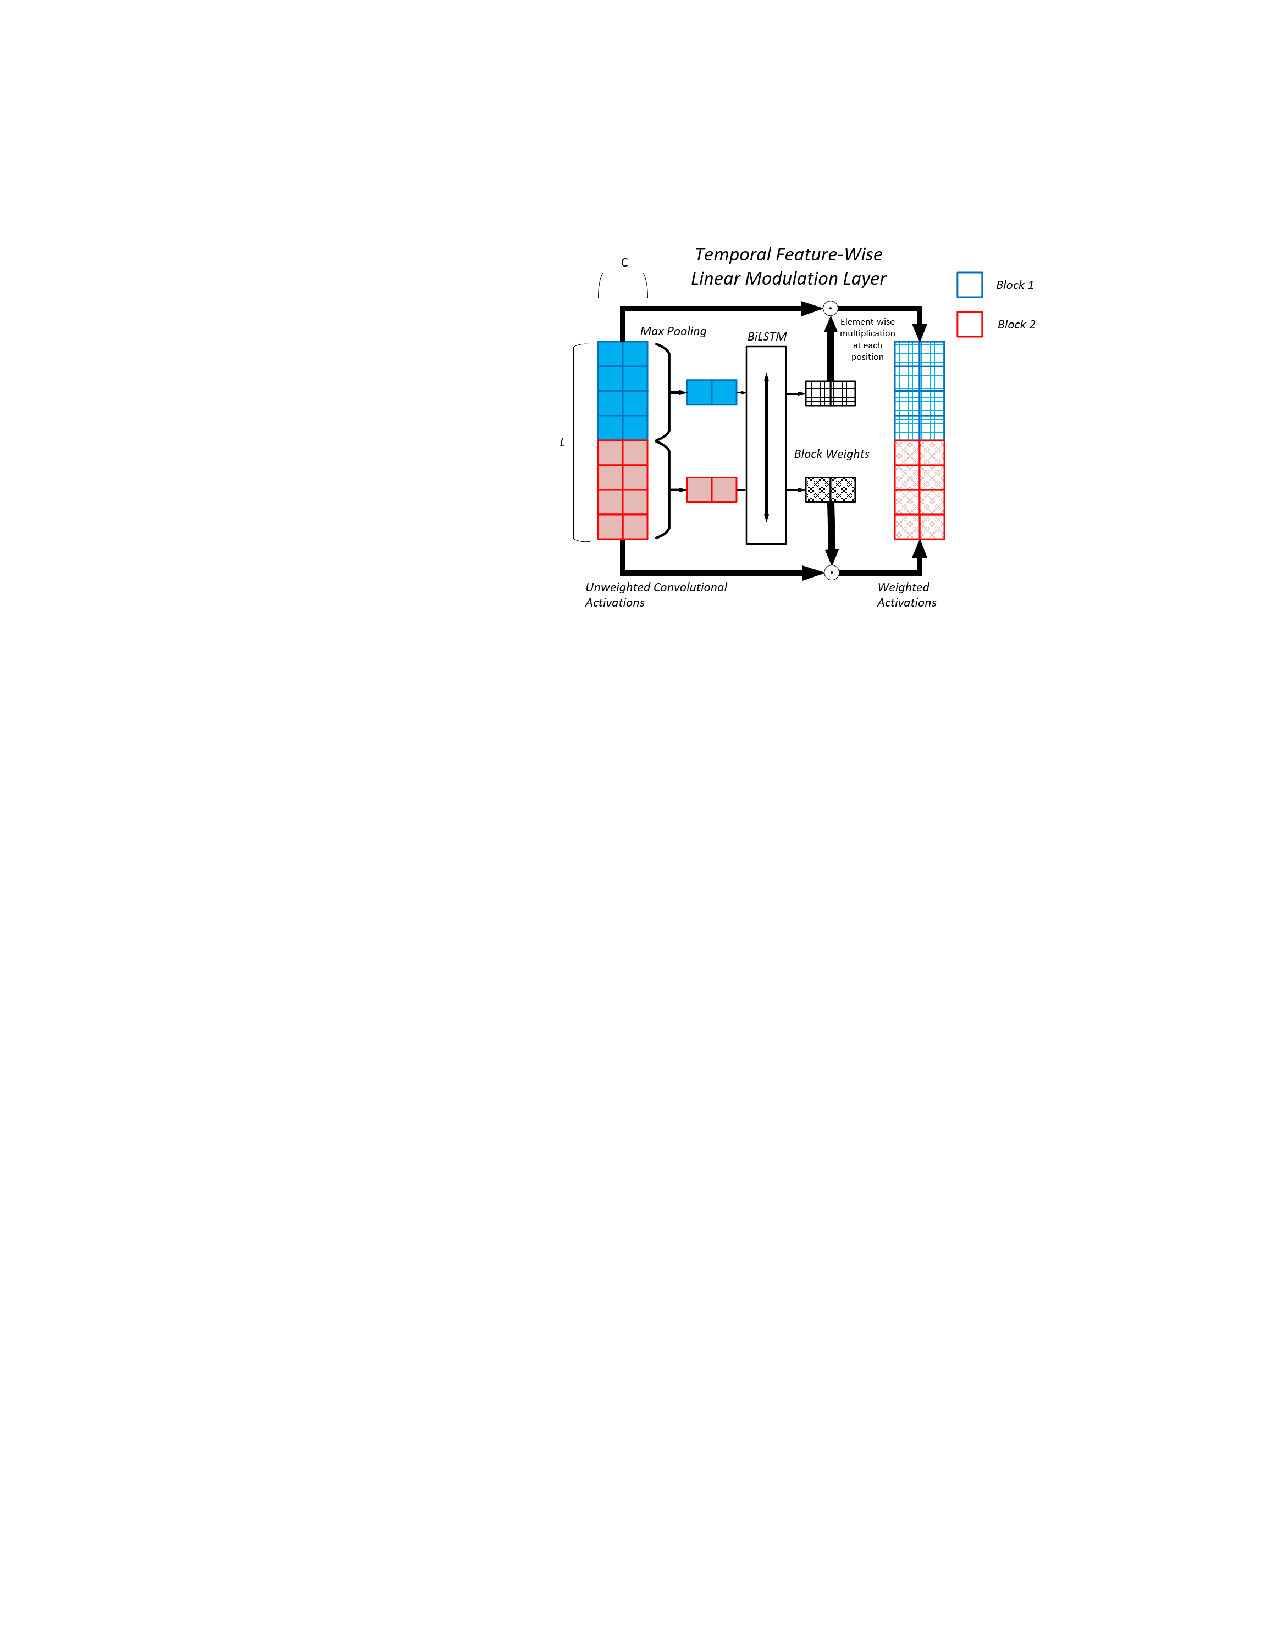
\includegraphics[scale=1.5]{img/tfilm_layer.pdf}  
		\captionsetup{margin=2cm}                         
		\caption{The \gls{tfilm} layer in detail. In this example the 1D tensor of convolutional activations has the following shape: $F \in \mathbf{R}^{8 \times 2}$. The 2 blocks are first processed by a Max Pooling layer (whit a pooling factor of 2) and then by the \gls{rnn}. Finally, the output of the recurrent network is used to modulate the convolutional layer.From \cite{birnbaum2019temporal}.}
		\label{fig:tflim_layer}                           
	\end{center}                                       
\end{figure}                                        
\noindent A significant difference between \gls{tfnet} and \gls{tfilm} lies in the fact that, while the former architecture is domain-dependent, the latter is domain-agnostic. Indeed, \gls{tfnet} performs domain-specific operations on signals such as \gls{dft}, while \gls{tfilm} layer does not require any of these operations. This fact has made the application of this model possible with regard to a wide variety of tasks. In general, \gls{tfilm} can be useful to process any sequential data. In fact, in the paper, the model’s effectiveness is demonstrated on three diverse domains: Text Classification, Audio \gls{sr} and Chromatin Immunoprecipitation Sequencing. The latter is a particular genomic experiment that consists in reconstructing high-quality measurements taken using a large set of probes (e.g., sequencing reads) from noisy measurements taken using a small set of probes. \\
It is interesting to point out that, for the researchers, Audio \gls{sr} and Chromatin Immunoprecipitation Sequencing tasks belong to the same class of generative modeling tasks, called \textit{time series super-resolution}. This problem consists in reconstructing a \gls{hr} signal from \gls{lr} measurements. \\
A brief overview of the model architecture proposed for time-series \gls{sr} tasks is given in Figure ~\ref{fig:tflim_architecture}. We can call this model \gls{tfilm} Net. \\
\begin{figure}[H]
	\begin{center}
		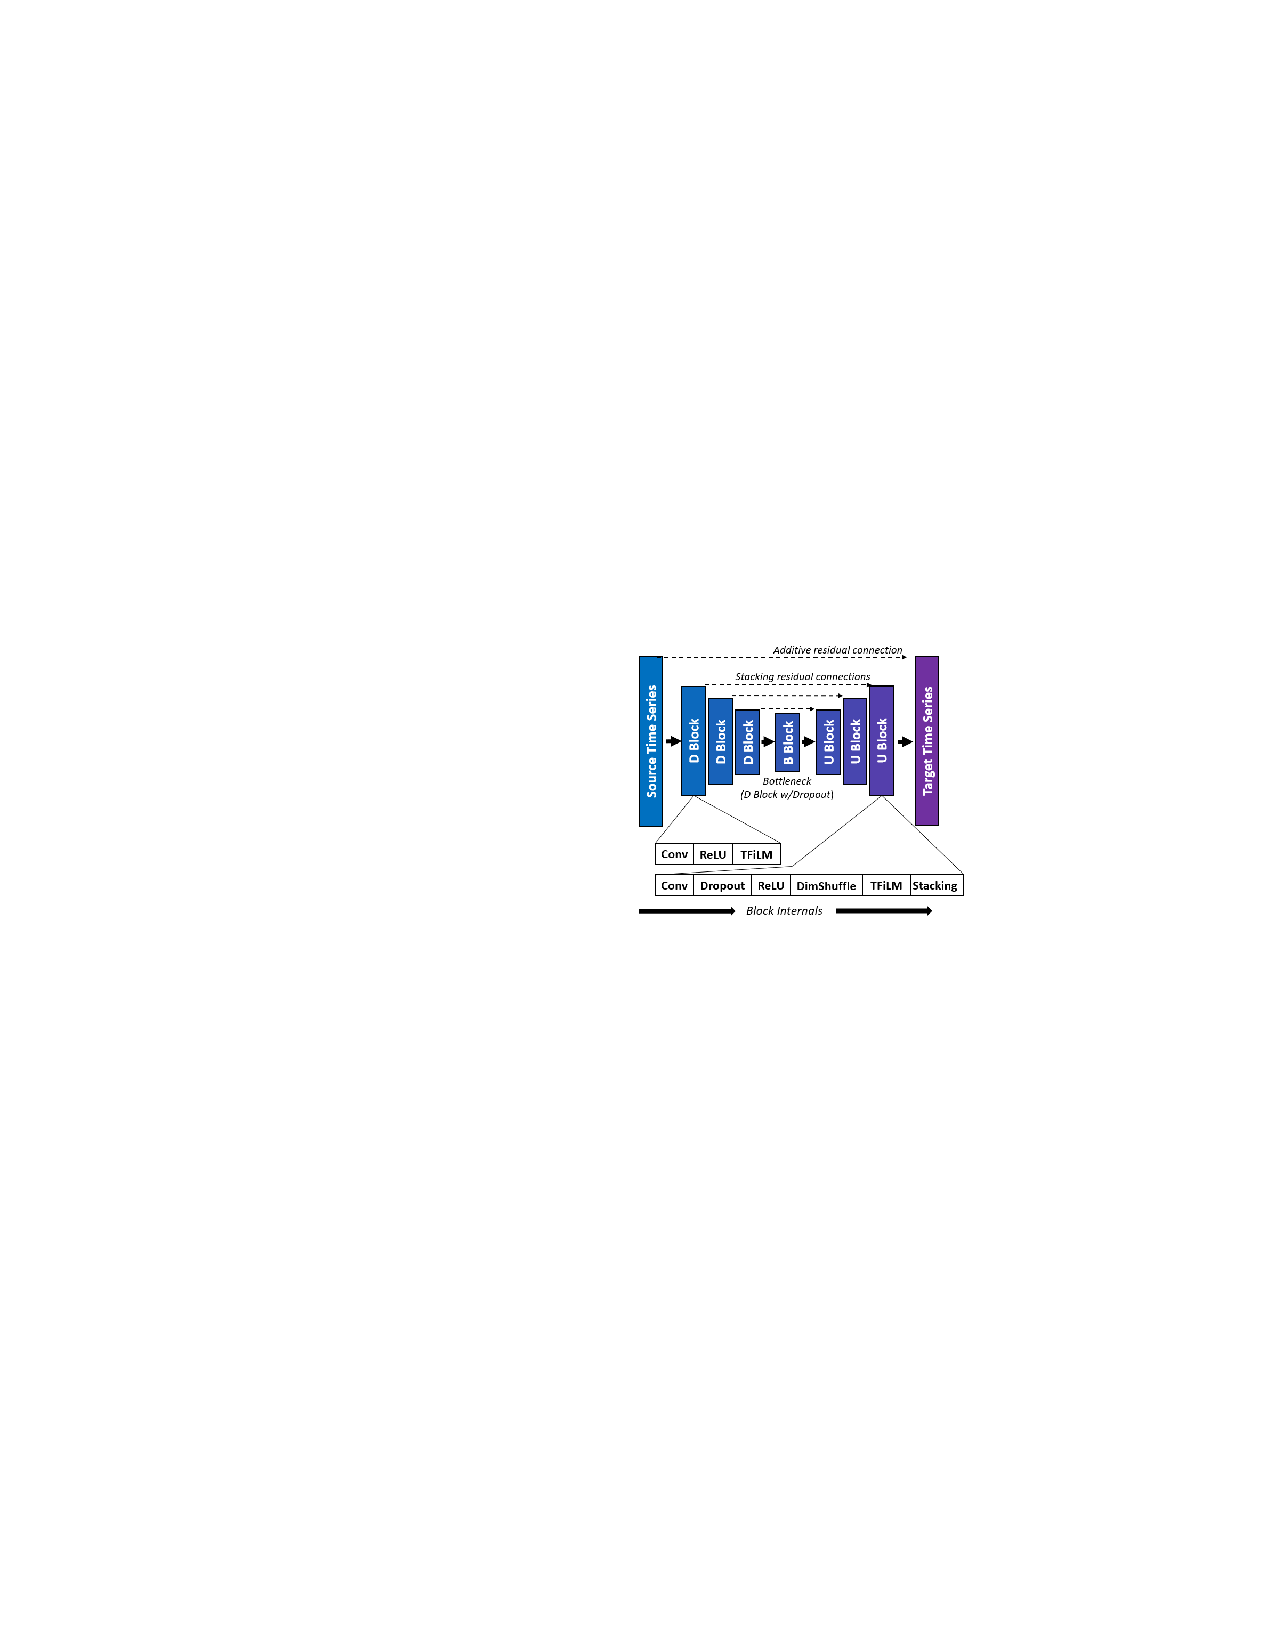
\includegraphics[scale=1.9]{img/tfilm_bottleneck.pdf}
		\captionsetup{margin=2cm}
		\caption{\textit{Top}: \gls{tfilm} Net architecture used for audio super-resolution. It consists of K downsampling blocks followed by a bottleneck layer and K upsampling blocks; features are reused via symmetric residual skip connections. \textit{Bottom}: Internal structure of downsampling and upsampling convolutional blocks. From \cite{birnbaum2019temporal}.}
		\label{fig:tflim_architecture}
	\end{center}
\end{figure}
\noindent As we can see, the architecture of \gls{tfilm} Net follows design patterns of AudioUNet (described in ~\ref{audiounet}). Indeed, we can recognize the bottleneck architecture, the subpixel layer, the use of B successive upsampling/downsampling blocks and the adoption of residual connections. This is not surprising because three of the authors are the same for both articles (i.e. \cite{kuleshov2017audio}, \cite{birnbaum2019temporal}).\\
However, there are several differences between AudioUNet and \gls{tfilm} Net, such as the use of recurrent and Feature-Wise Linear Modulation layers. Moreover, while AudioUNet uses standard convolutional layers, \gls{tfilm} Net exploits dilated convolutional approaches to extract highly representative features from a wider receptive field. Dilated convolution is described in detail in section ~\ref{dilated_conv}. \\
As for implementation details, it is essential to note that the authors instantiated the model with $K = 4$ (recalling that $K$ is the number of  upsampling and downsampling blocks). Another important hyperparameter is the number of \gls{tfilm} layer blocks $L = \frac{T}{B}$. In this regard, the block length values $B$ are adjusted for each layer so that the ratio between the temporal dimension $T$ and $B$ is always 32. In other words, the number of blocks $L$ is set to 32 in each \gls{tfilm} layer. \\
In order to facilitate understanding of the whole process, a graphical representation of the entire entire pipeline of \gls{tfilm} Net is proposed in Figure ~\ref{fig:tfilm_pipeline}. \\
\begin{figure}[!htb]
	\begin{center}
		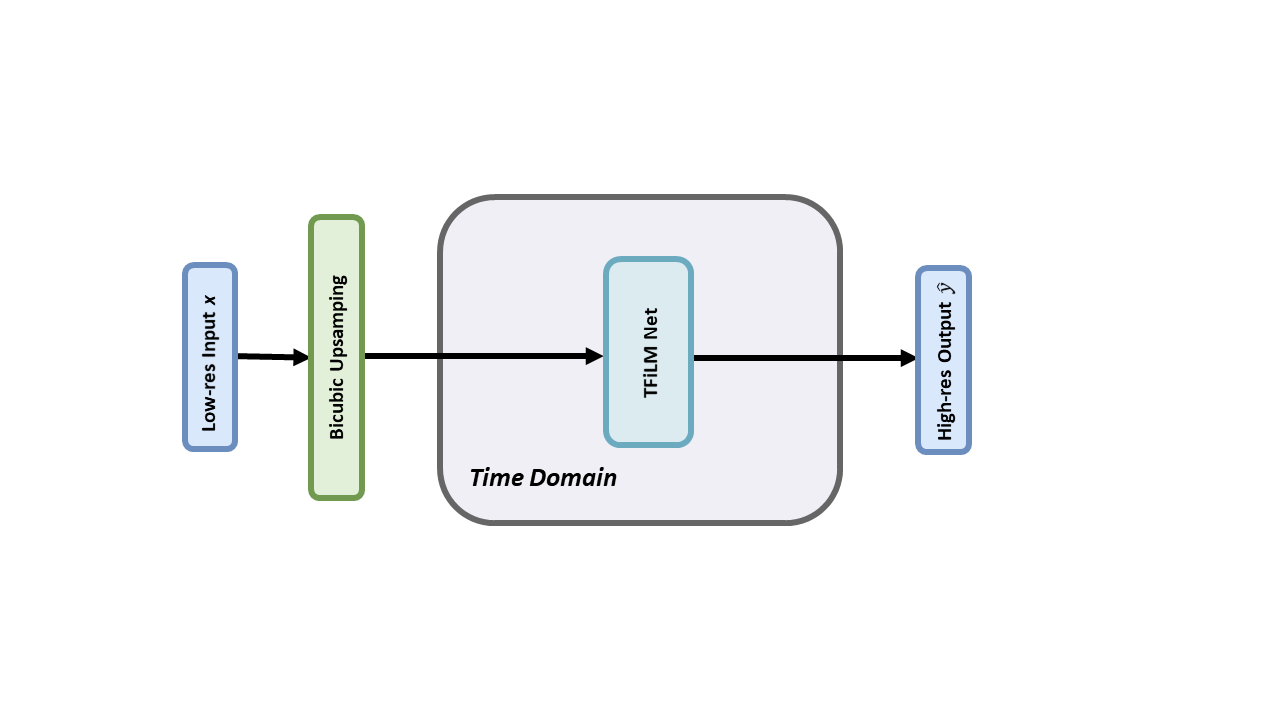
\includegraphics[scale=0.48]{img/tfilm_pipeline.png}
		\captionsetup{margin=2cm}
		\caption{Overall pipeline of \gls{tfilm} Net. The system integrates convolutional and recurrent layers to efficiently incorporate long-term input dependencies by operating in the time-domain.} 
		\label{fig:tfilm_pipeline}
	\end{center}
\end{figure}


\subsection{Dilated Convolution} \label{dilated_conv}
\noindent To further increase the receptive field of convolutional layers, authors use dilated convolutions with a dilation factor of 2. \\
Dilated convolution \cite{yu2015multi} is a generalization of the familiar discrete-convolution (that can be considered as the 1-dilated convolution). In summary, this particular type of convolution, defines a spacing between the values in a kernel. This allows to increase the receptive field of a convolution, without a corresponding increase in the number of trainable parameters. Therefore, the choice to use this type of layer is perfectly consistent with the objectives of this work.\\
For example, considering the two-dimensional convolution, a $3 \times 3$ kernel with a dilation rate of 2 results to have the same receptive field of view as a $7 \times 7$ kernel. A graphical representation of this example is provided in Figure ~\ref{fig:dilated_conv}.

\begin{figure}[H]
	\begin{center}
		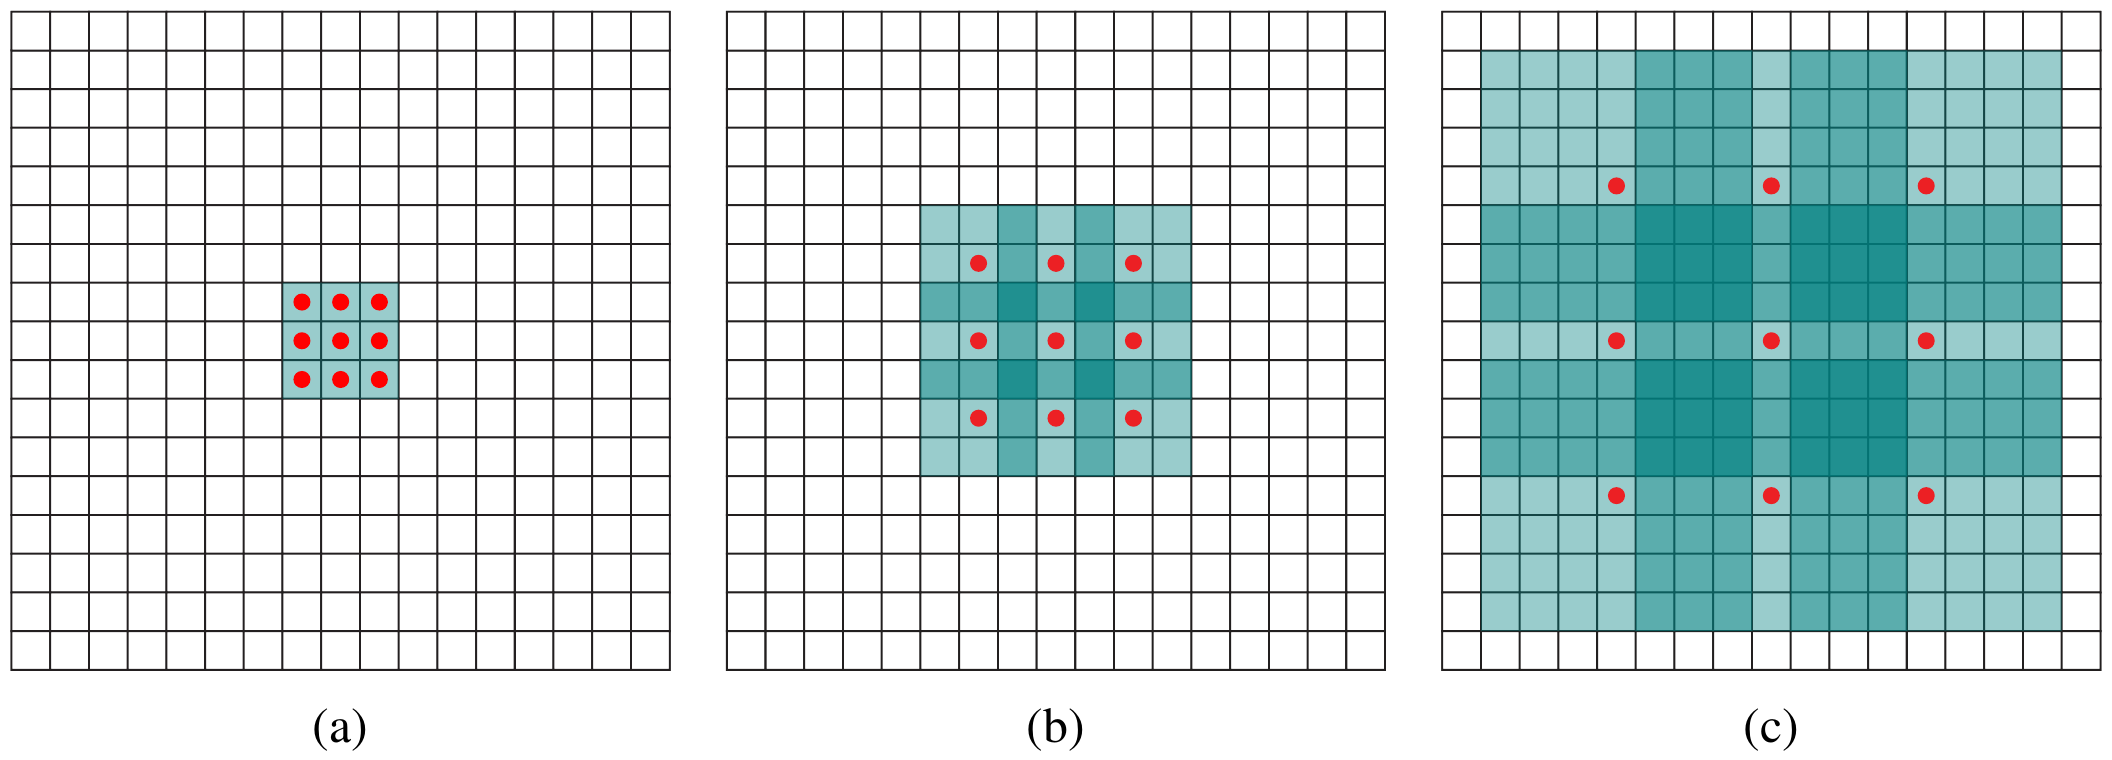
\includegraphics[scale=.21]{img/dilated_conv.png}
		\captionsetup{margin=2cm}
		\caption{(a) 1-Dilated Convolution has a receptive field of $3 \times 3$. (b) 2-Dilated Convolution has a receptive field of $7 \times 7$. (c) 4-Dilated Convolution has a receptive field of $15 \times 15$. The number of parameters associated with each layer is identical. The receptive field grows exponentially while the number of parameters grows linearly. From \cite{yu2015multi}.}
		\label{fig:dilated_conv}
	\end{center}
\end{figure}

\subsection{Feature-Wise Linear Modulation} \label{film}
As the name suggests, a \gls{film} layer applies a feature-wise affine transformation, based on conditioning informations of an auxiliary input $z \in \mathbf{Z}$. \gls{film} can be thought of as a generalization of Conditional Normalization \cite{dumoulin2016learned}, that is used in \gls{dl} for stabilizing the training of the models. Batch Normalization and \gls{film} are formally described as follows. \\
Consider a tensor of 1D multichannel convolutional activations $F \in \mathbf{R}^{T \times C}$ (where $T$ is the time axis and $C$ is equal to the number of channels). The batch normalization  rescales $F$ and applies an affine transformation, so that it produces an output $F^{\prime} \in \mathbf{R}^{T \times C}$ whose $(t, c)$ -th output elements are described in Equation \ref{eq:batch_norm}:
\begin{align}\label{eq:batch_norm}
	\begin{array}{c}
		F_{t, c}^{\prime}=\gamma_{c} \hat{F}_{t, c}+\beta_{c}
	\end{array}
\end{align}
Where $\hat{F}_{t, c}$ is defined as follows.
\begin{align}\label{eq:batch_norm2}
	\begin{array}{c}
		\hat{F}_{t, c}=\frac{F_{t, c}-\mu_{c}}{\sigma_{c}+\epsilon} 
	\end{array}
\end{align}
From the notational point of view, it is important to define $\mu_{c}, \sigma_{c}$ that are, respectively, the estimates of the mean and standard deviation for the $c$ -th channel. As for $\gamma, \beta \in \mathbf{R}^{C}$, they are trainable parameters. \\
\gls{film} \cite{perez2018film} extends this idea by allowing $\gamma, \beta$ to be functions $\gamma, \beta: \mathcal{Z} \rightarrow \mathbf{R}^{C}$ of an auxiliary input $z \in \mathcal{Z}$. This technique is domain independent, i.e. can be used for a wide variety of applications. For example, in feed-forward image style transfer \cite{dumoulin2016learned}, $z$ is an image defining a new style; by using different $\gamma(z), \beta(z)$ for each $z$, the same feed-forward network (using the same weights) can apply different styles to a target image. \gls{film} has also obtained significant results in speech recognition \cite{kim2017dynamic} and image classification \cite{hu2018squeeze}. 

\section{Proposed Model Architecture}
The main objective of this paragraph is to provide a detailed explanation of the proposed model, that aims to combine elements of both \gls{tfnet} and \gls{tfilm} Net in an effective way.\\
Taking inspiration from \gls{tfnet}, the proposed deep network architecture is made of two branches: one for time-domain and one for spectral-domain processing. Indeed, Lim, Yeh \textit{et al.} demonstrate that this strategy helps the model to better estimate the high-frequency content of the signal. However, their approach is fully convolutional. In this regard, Birnbaum, Kuleshov \textit{et al.} highlight that \gls{cnn}-based methods have intrinsic limitations when applied to sequential data. As mentioned before, \gls{cnn}s are not effective for capturing long-term dependency due to the relatively high computational requirements of large receptive fields. To address this problem, the proposed model incorporates \gls{tfilm} components in the processing. More specifically, the AudioUNet components used in \gls{tfnet} are replaced with the \gls{tfilm} layers, that can capture long-range input dependencies by modulating the activations of a convolutional layer through a \gls{rnn}. \\
To further capture the low-high frequency dependency in the signal, it is decided to keep the spectral replicator layer in the model architecture. It would also be interesting to evaluate the impact of this operation by training another model that does not have this layer in its pipeline.
\\ To sum up, the proposed approach mainly aims to overcome the limitations of the \gls{tfnet} architecture, with which it shares a similar pipeline. Indeed, key components, such as the Spectral Replicator and the Spectral Fusion Layer, are maintained in the system. \\
A graphical representation of the model pipeline is provided in Figure ~\ref{fig:proposed_pipeline}. \\
From a notational point of view, the term "Slim \gls{tfilm} Net" indicates that the original dimension of the network is reduced by halving the number of filters in each branch. \\
The Slim \gls{tfilm} Nets in the two branches are dimensionally equivalent: both the size and the number of filters applied in each layer are the same. What changes is the length of the input sequence. Indeed, as in the case of \gls{tfnet} model, a \gls{dft} on the sequence is computed to pass from the time to the spectral domain. Because of this, the spectral branch processes a signal that is half the length of the time branch signal.  
\begin{figure}[!htb]
	\begin{center}
		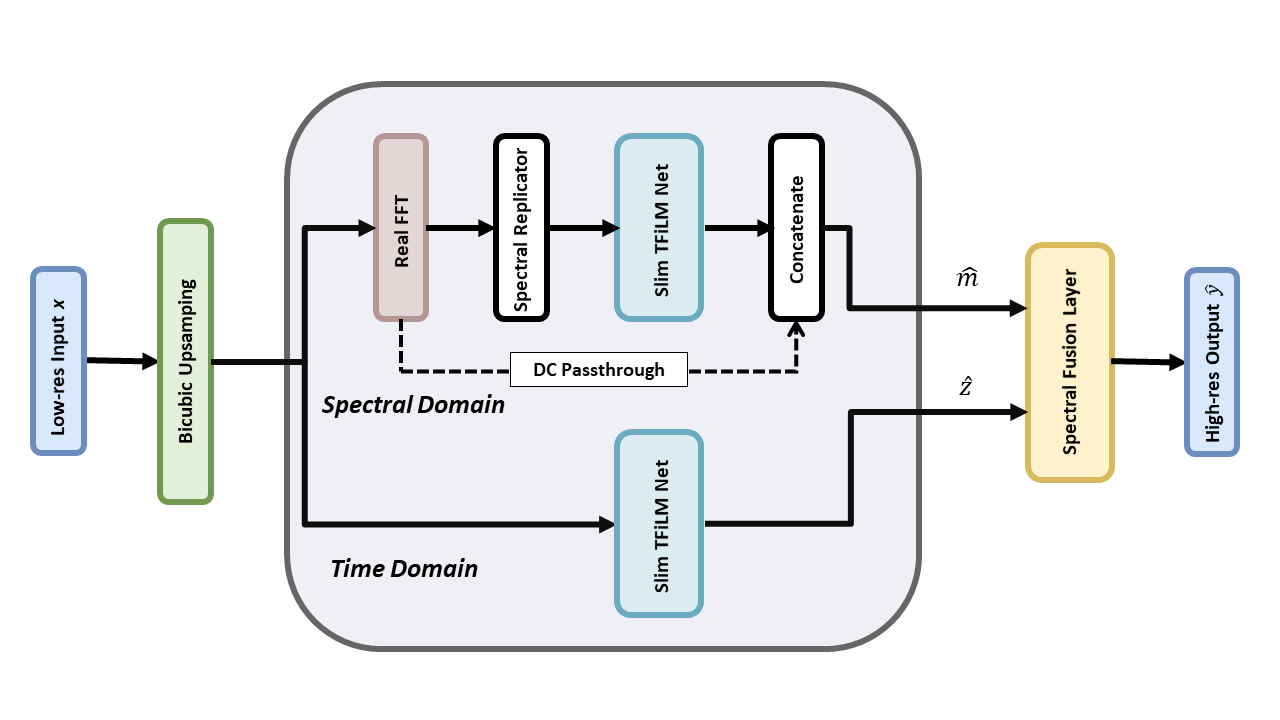
\includegraphics[scale=0.48]{img/proposed_pipeline.png}
		\captionsetup{margin=2cm}
		\caption{Overall pipeline of the proposed model. On one hand, the system maintains the branching structure of \gls{tfnet} that allows to processes audio in both time and frequency domain. On the other hand, the model uses \gls{tfilm} Net to predict both the audio reconstruction and the spectral magnitude.} 
		\label{fig:proposed_pipeline}
	\end{center}
\end{figure}


\section{Implementation details} \label{implementation_details}
As mentioned earlier, in order to identify which is the best architecture between different models, it is important to establish a context that is as fair as possible for the comparison. In this sense, the number of trainable parameters can serve as a benchmark criterion for comparing different results. \\ Here, however, there is a problem. The available computational resources do not allow to propose and train a model with the same dimensions of \gls{tfnet} and \gls{tfilm} Net. In fact, these two models have roughly 35M parameters, while the available resources allow to train models with approximately 22M parameters. This gap is too wide to compare the results reported in the papers \cite{lim2018time}, \cite{birnbaum2019temporal} with the novel model architecture. For this reason, it is decided to reduce the dimensionality and re-train both \gls{tfnet} and \gls{tfilm} Net. \\
To achieve this goal, we proceed in the following way. Recalling that the \gls{dl} components of the models, i.e. AudioUNet and \gls{tfilm}, have a bottleneck architecture that consists of downsampling and upsampling blocks, it is decided to remove the last layer (which is the largest) from all of these components. By doing so, the number of upsampling and downsampling blocks (called B in \ref{audiounet} and K in \ref{tfilm}) is reduced from 4 to 3.\\
This change is enough to enable the model training within the computational limits available to us. Therefore, all other architectural characteristics of the models remain faithful to the original implementation.\\
Another difference from the papers \cite{lim2018time}, \cite{birnbaum2019temporal} concerns the data used for the training: the dataset is the same as the one used in both papers, but in this project we sample a subset of recordings because of dimensionality issues. This is explained in more details in Chapter \ref{chap:exp_results}. 

 %read tex file from chapters folder 

\chapter{Experimental Results} \label{chap:exp_results}
In this chapter, the results of the experiments performed to validate and test the methods presented in Chapter \ref{chap:methods} are discussed with the aim to establish the best model architecture. In order to do so, it is first necessary to briefly introduce the experimental setup on which this model comparison is conducted. \\
Each model is evaluated under two different regimes: \textit{Multi-Speaker} and \textit{Single-Speaker}. The former task aims to develop a system able to generalize the artificial \gls{bwe} to both female and male speakers with different accents. The latter one, as the name suggests, takes into account only data coming from a single speaker. Specifically for our experiments, the first speaker of the \gls{vctk} dataset. Both tasks are addressed in the reference papers too (\cite{lim2018time}, \cite{birnbaum2019temporal}). \\
As for software tools, the whole project is written in Python. This programming language is well suited to achieve the desired development purposes, since it offers a diverse set of tools for both \gls{dsp} and \gls{dl} applications. The main packages used in this work include Tensorflow, Scipy and Librosa. \\
%As motivated in the previous chapter, it is worth noting that this project requires large computational resources that arise from both the dataset size and the models' number of parameters. \\
We use Google Colaboratory (Colab), a cloud-based service accessible through a web browser. The key advantage of this environment is that it provides up to 25GB of RAM, and a free access to the high-end GPUs. This helps in reducing the computational time as GPUs are very powerful for massively parallel computations, such as the ones required for tensors (signals' data structure) processing.

\begin{figure}[H]
	\begin{subfigure}{.25\textwidth}
		\centering
		
\includegraphics[width=.7\linewidth]{img/colab_logo.png}
		\label{fig:colab_logo}
	\end{subfigure}%
	\begin{subfigure}{.25\textwidth}
		\centering
		
\includegraphics[width=.6\linewidth]{img/tensorflow_logo.png}
		\label{fig:tensorflow_logo}
	\end{subfigure}%
	\begin{subfigure}{.25\textwidth}
		\centering
		
\includegraphics[width=1.1\linewidth]{img/librosa_logo.png}
		\label{fig:librosa_logo}
	\end{subfigure}%
	\begin{subfigure}{.25\textwidth}
		\centering
		
\includegraphics[width=.55\linewidth]{img/scipy_logo.png}
		\label{fig:scipy_logo}
	\end{subfigure}
	\caption{From the left, the logos of Colab, Tensorflow, Librosa and Scipy.}
	\label{fig:fig}
\end{figure}

\section{Experimental Setup}
This paragraph aims to provide a clear specification of the experimental setup. A full description of the dataset and its preparation is provided along with the metrics used to evaluate the models. 

\subsection{Dataset and preparation}
Experiments reported in this thesis are undertaken using the most popular dataset for the audio SR task, i.e. \gls{vctk} \cite{yamagishi2019cstr}. In recent years, many researchers have used it (see e.g., \cite{birnbaum2019temporal}, \cite{lim2018time}, \cite{eskimez2019speech}, \cite{wang2018speech}), to such an extent that we can now consider this dataset as a benchmark for the \gls{bwe} problem. \\
This \gls{vctk} Corpus contains approximately 44 hours of speech data uttered by 109 English speakers, each of whom reads out about 400 different sentences. The dataset was initially designed for training Text-to-Speech synthesis systems. In fact, each recording is associated with the corresponding textual transcription. This data are used in this work in order to evaluate models' performance over the \gls{stt} task, whose details are discussed in section \ref{eval_methods}. \\
The \gls{vctk} Corpus encompasses speakers with various accents, as shown in Figure \ref{fig:accents_speakers}. \\
\begin{figure}[!htb]
	\begin{center}
		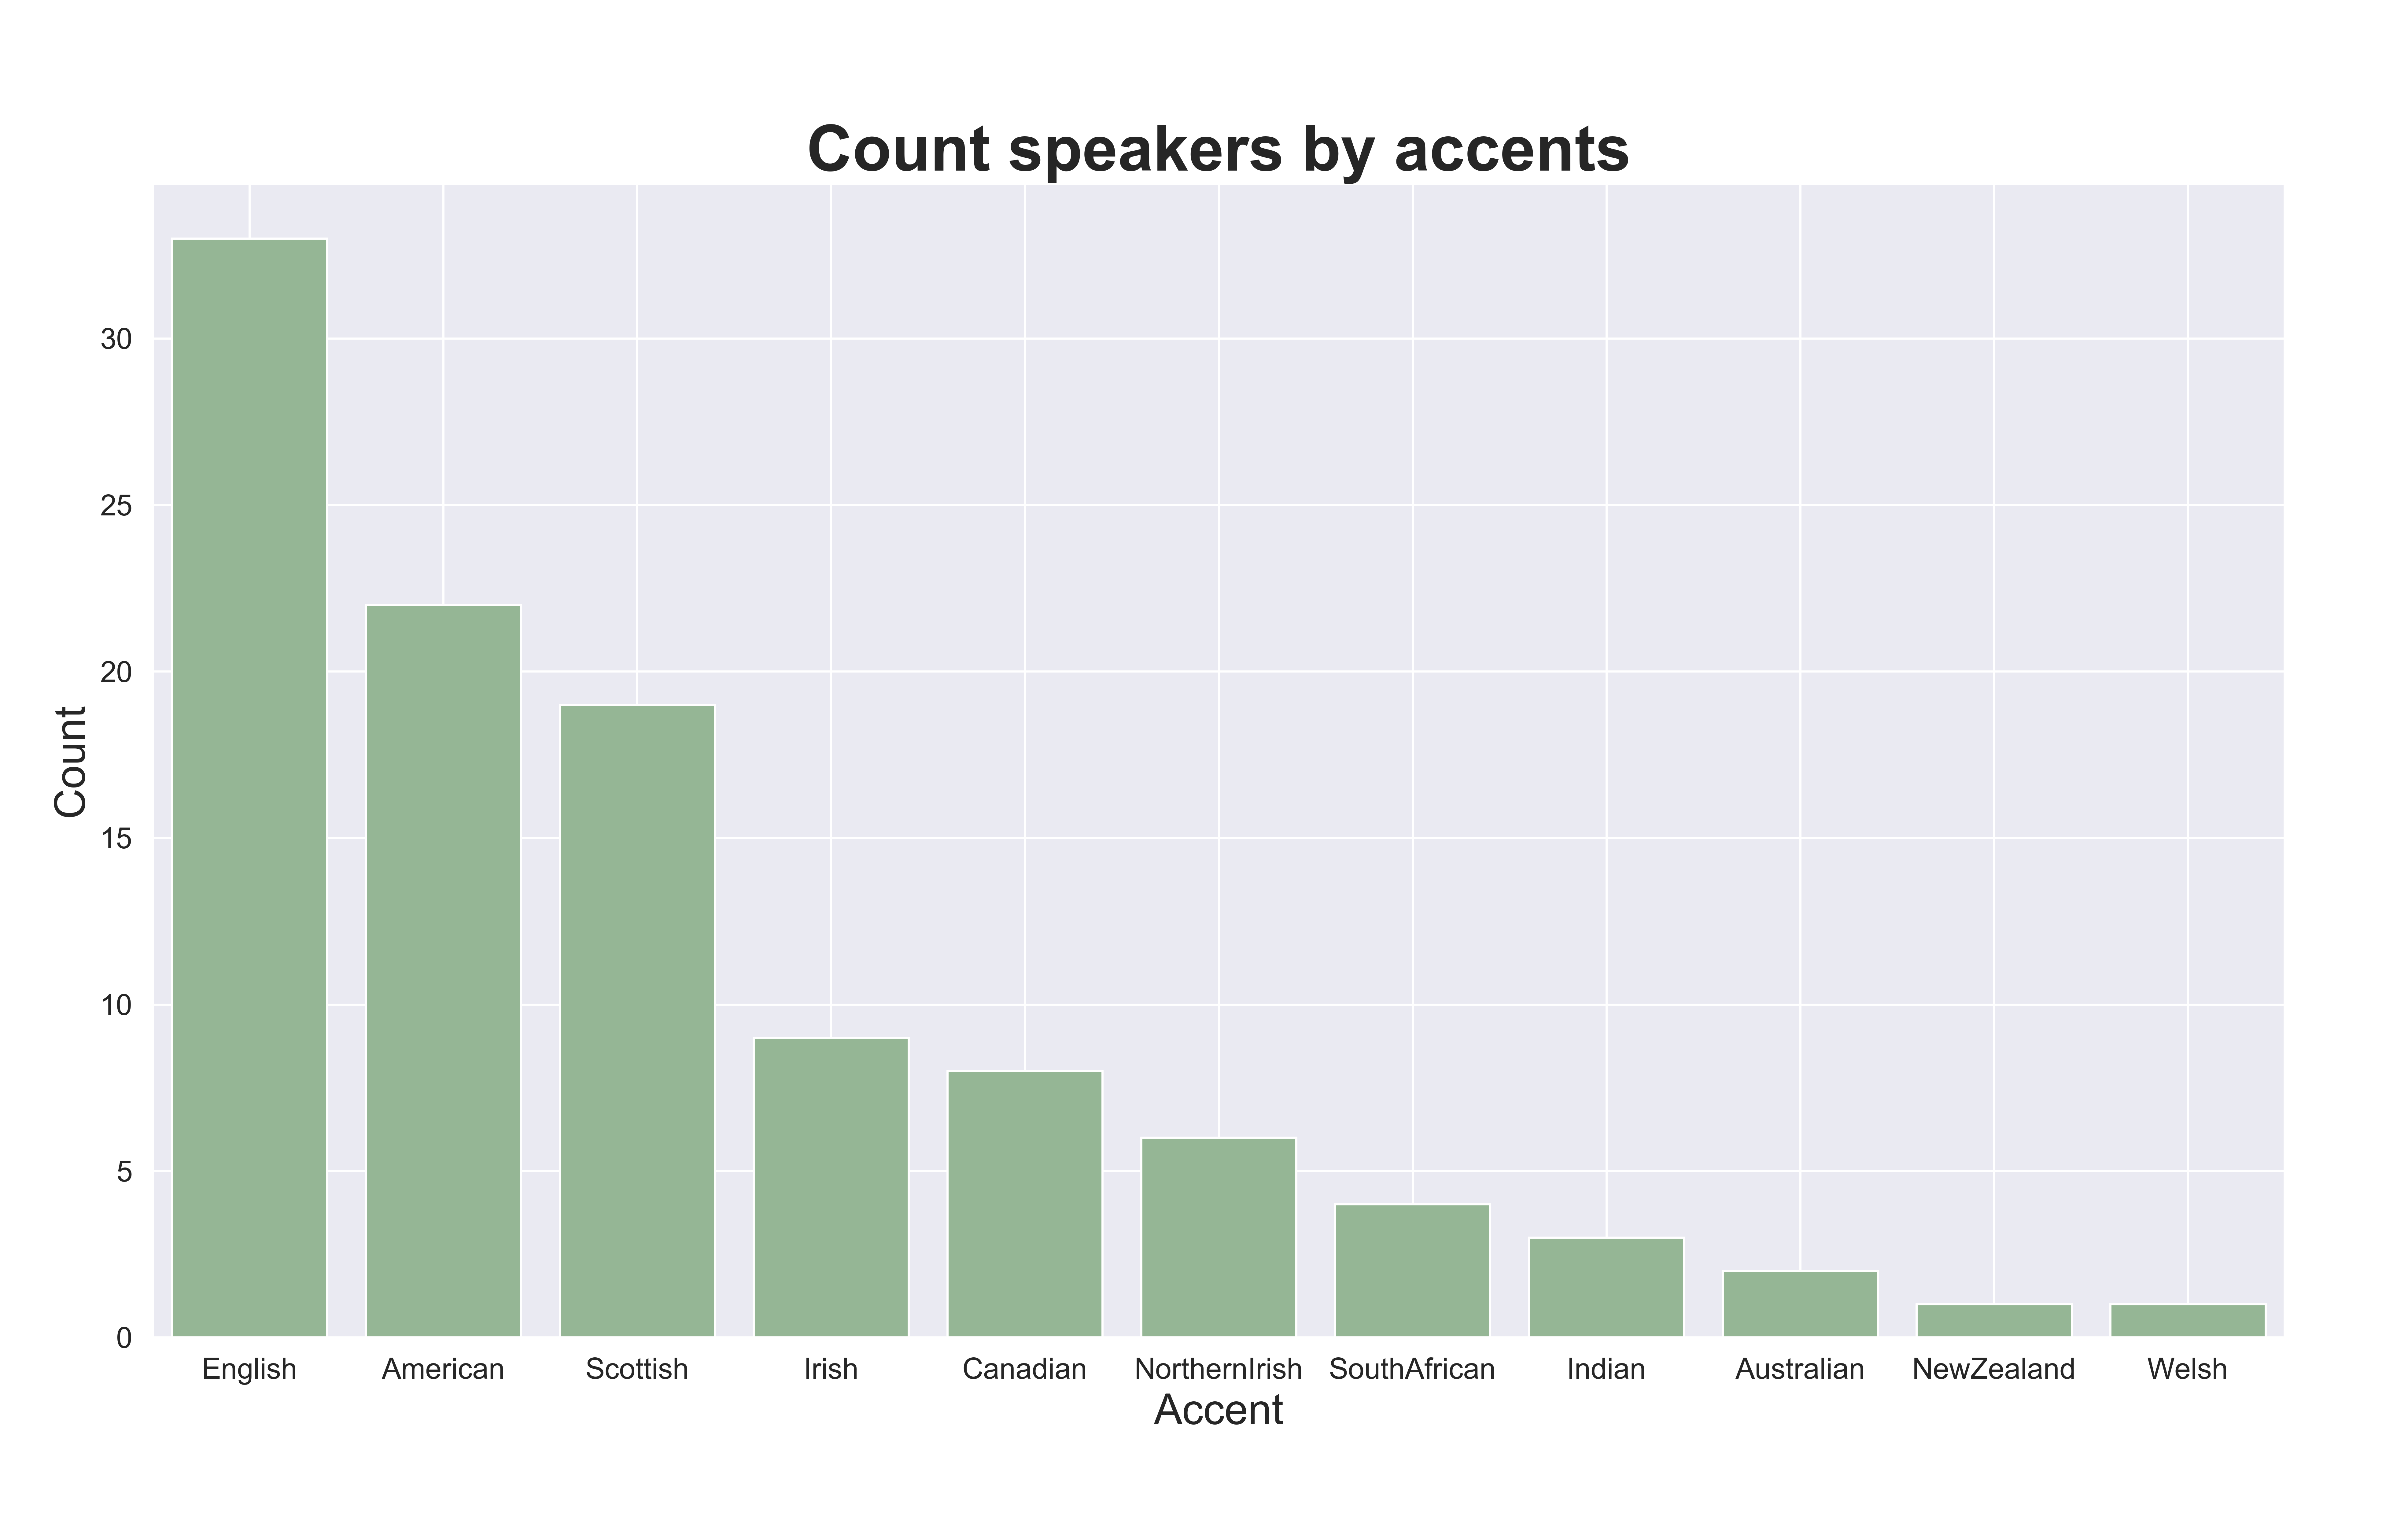
\includegraphics[scale=0.4]{img/count_speakers_by_accents.png}
		\caption{Bar chart showing the count of speakers in \gls{vctk} dataset based on their accent.}
		\label{fig:accents_speakers}
	\end{center}
\end{figure}
\noindent All speech data are clean, and they were originally recorded using an identical recording setup, i.e. 96 kHz sampling frequency at 24 bits in the same room, with the same microphone. All recordings were finally converted into 16 bits and downsampled to 48 kHz; this is the quality of data available online. \\
All recordings are further downsampled to 16 kHz for this project: it is possible to consider this sampling rate as $R_2$, i.e. the one that defines the ground truth $y = (y_{1/R_2}, y_{2/R_2}, \dots, y_{R_2S/R_2})$. It follows that, for a scaling ratio of $4 \times$, $R_1$ is equal to 4 kHz. It is noticeable that 16 kHz can be reasonably considered as a high quality standard for speech processing applications \cite{steidl2009automatic}; suffice to say that a standard telephone audio has a sampling rate of 8 kHz and 16-bit precision \cite{kamath2019automatic}. \\
As previously motivated, computational resources for this project are limited: in the multi-speaker task, it is not possible to use the whole dataset, as both reference papers, i.e. \cite{lim2018time} and \cite{birnbaum2019temporal}, do. In particular, authors of the reference papers train the models for this task on the first 100 \gls{vctk} speakers and test on the 9 remaining ones. We re-train their models, and the proposed system, on a sample of 40 speakers. However, the test set used in this project remains the same as the one used in both articles. By doing so, the comparison with newly developed models is placed in a fair context. Furthermore, the difference between the performance ~-~ of \gls{tfnet} and \gls{tfilm} ~-~ obtained in the original works and those obtained in this project, can be used to measure the negative impact that a drastic reduction in the dimensionality of the problem inevitably has on the performance of the system. \\
In addition, we also make use of a validation set, the importance of which is explained in section \ref{training_details}. It is important to highlight that there is no speaker overlap between train, validation and test partitions. This setting is selected in order to reduce performance over-estimation due to potential auto-correlations among different observations pertaining to the same speaker. \\
Both train and validation sets are sampled in a principled way: the main goal of this sample design is to maximize the model robustness with respect to the main factors of variation. When analyzing a speech recording, important factors concern, for example, the speaker’s sex and their accent. Thus, speakers are selected in order to ensure a balanced distribution by gender and a heterogeneous distribution of accents. From a theoretical point of view, this should encourage the creation of a \gls{dl} model that is robust with respect to variations of accent and gender. \\
The sampling performed also reflects the age distribution of the original dataset (especially for the female gender), as can be seen from Figure \ref{fig:age_dataset}. \\
\begin{figure}[H]
	\begin{center}
		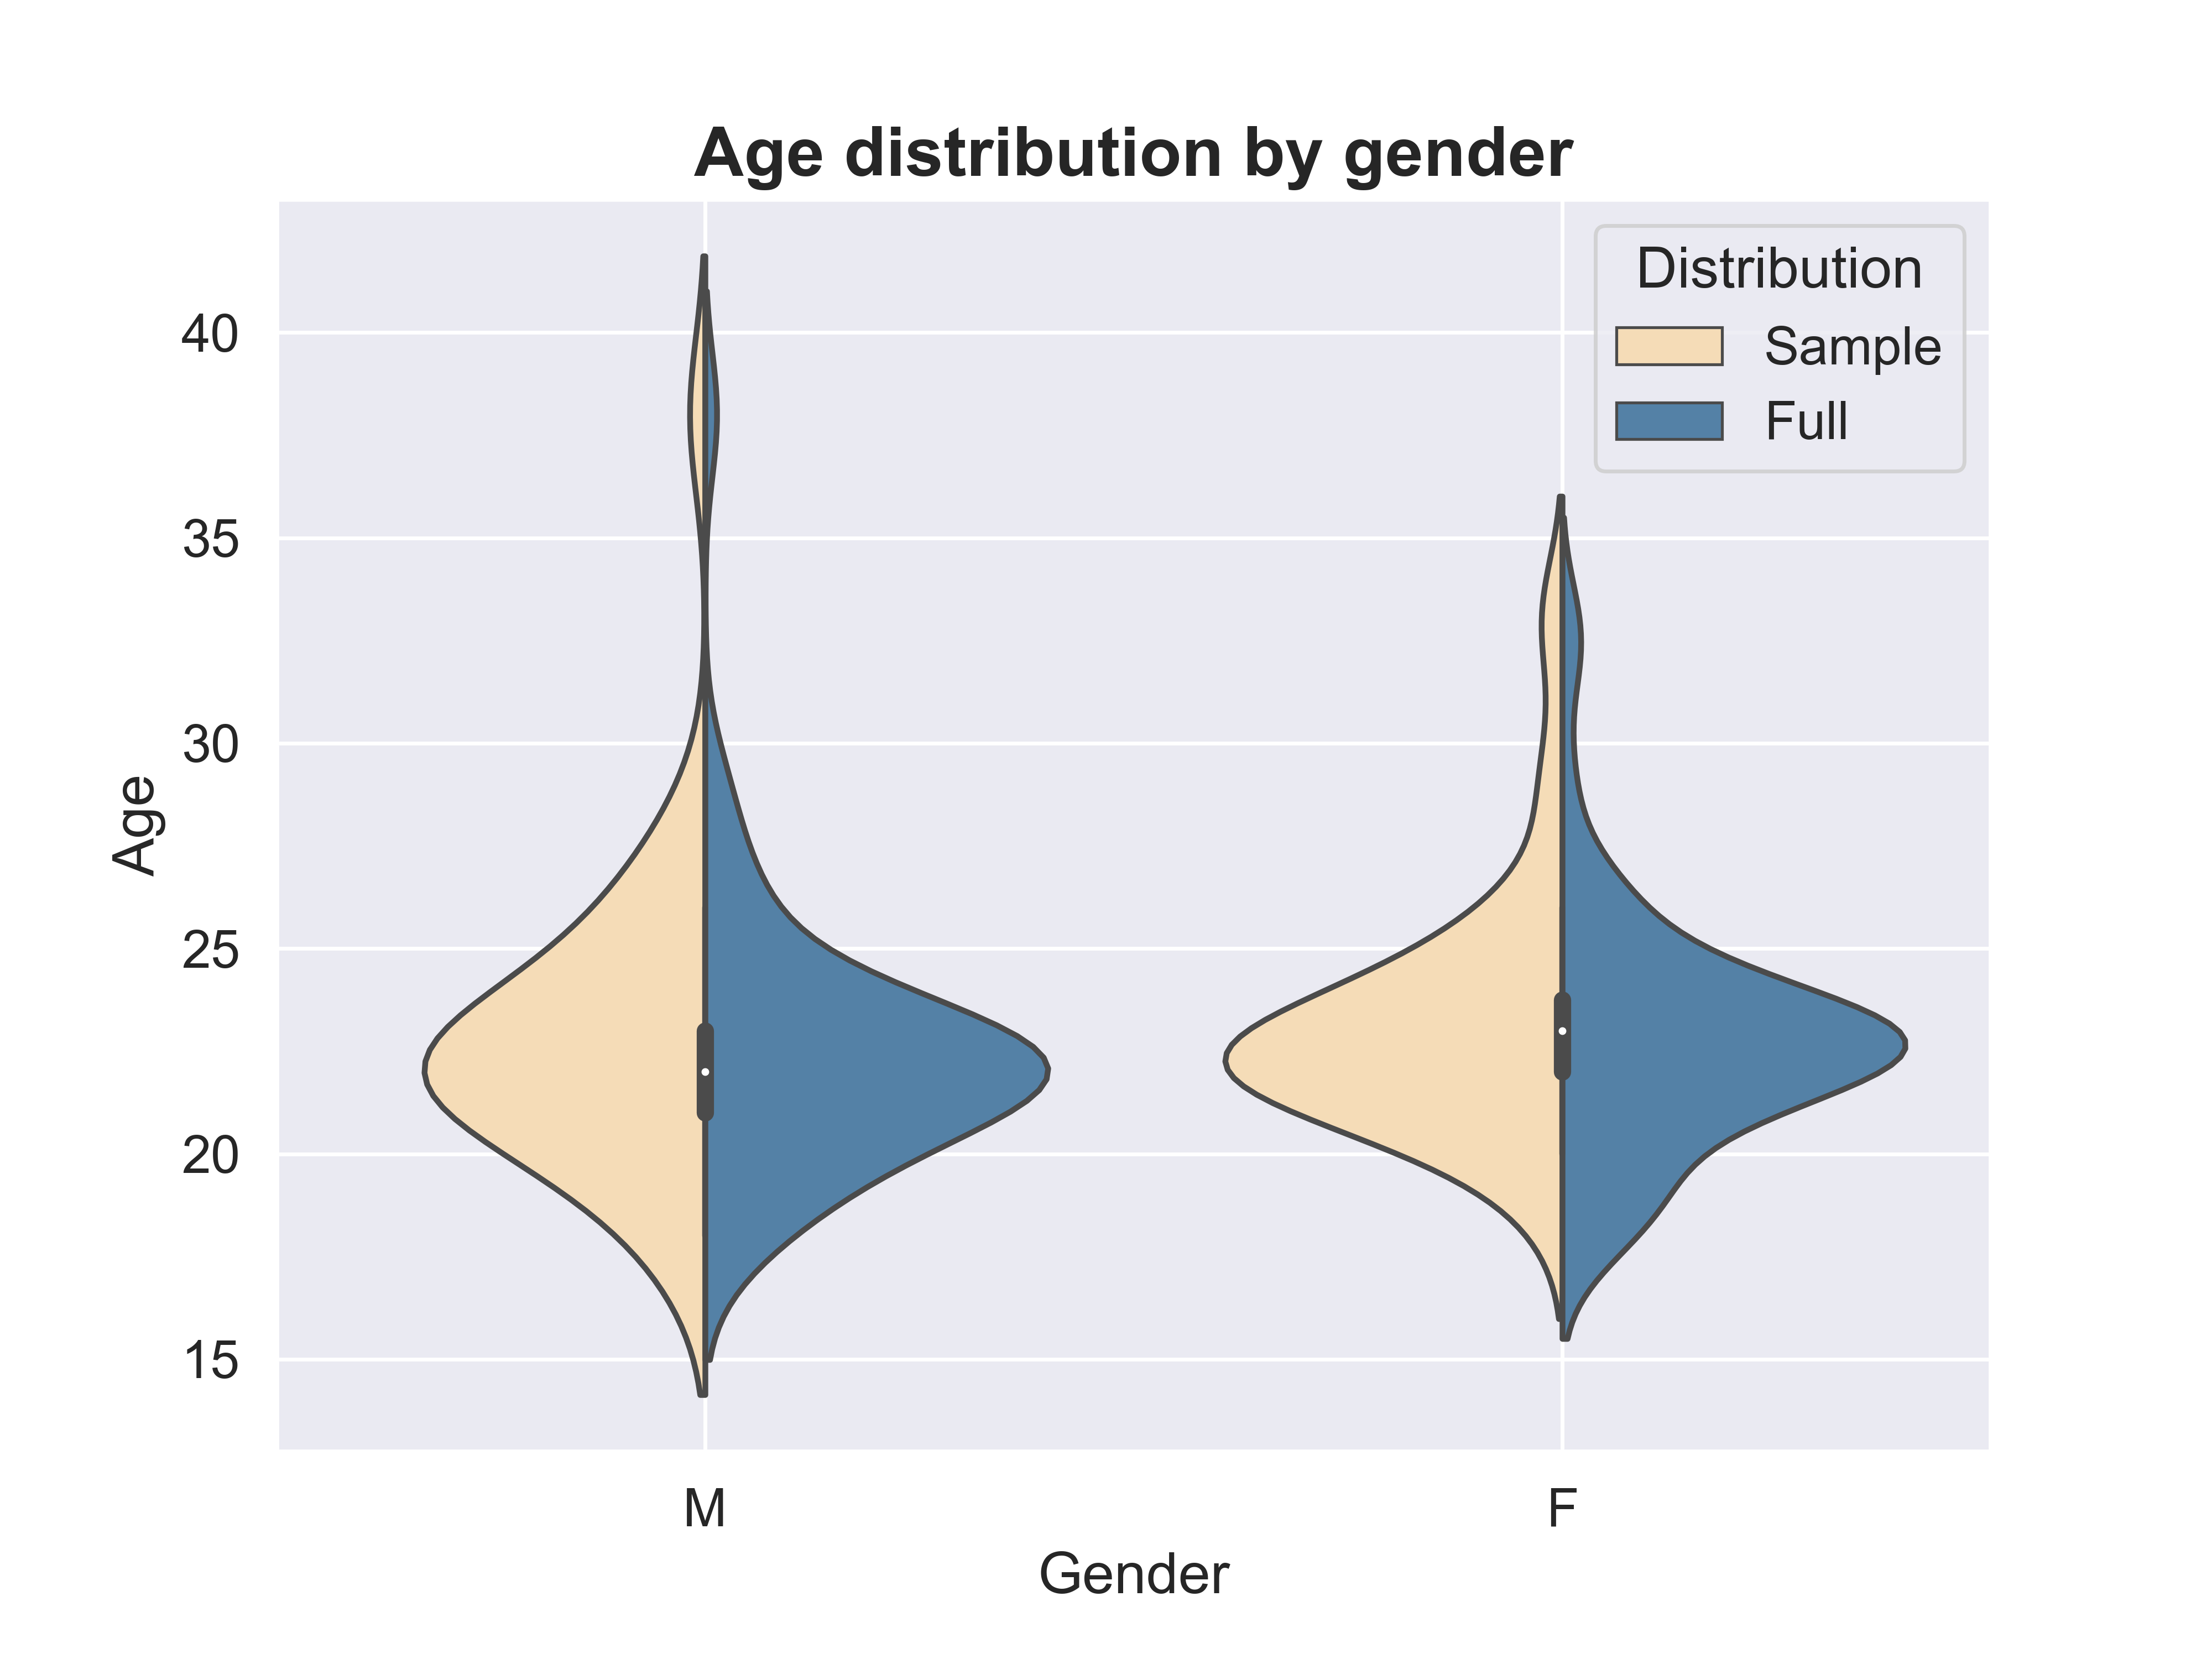
\includegraphics[scale=0.6]{img/age_distribution_by_gender.png}
		\caption{Violin plot showing the age distribution of speakers in \gls{vctk} dataset based on level of gender.}
		\label{fig:age_dataset}
	\end{center}
\end{figure}
\noindent As for the single-speaker task, we follow the previous works \cite{lim2018time} by indicating with "\gls{vctk}s" the subset of the whole dataset which only includes the first speaker. It is worth mentioning that this subset does not belong to the set of data used to train, validate or test the models for the multi-speaker task. The train-test split criterion is the same as the one used in both reference papers, i.e. a standard 85\% training - 15\% test split with no audio-clips overlap. \\
Furthermore, we keep the same data structure used in both \gls{tfnet} and \gls{tfilm} works: we extract from each recording a set of one-dimensional vectors of length 8192. In particular, each audio clip is divided into several subsequences by the use of a sliding window approach such that each subsequence (or \textit{patch}) shares 75\% of its content with the previous one. Therefore, recalling that the sampling rate of our data is 16 kHz, this corresponds to patches of approximately 500ms with the start of every patch 125 ms apart from the previous one. \\
The corresponding \gls{lr} patches are obtained by downsampling the original recordings. In particular, we use an order 8 Chebyshev type I low-pass filter with cut-off frequency at $R_{1_{lim}}$. Recalling that in our setup we have $R_1 = 4$ kHz, it follows that $R_{1_{lim}} = 2$ kHz. In other words, the low-pass filter allows to obtain the \gls{lr} signal by cutting off the frequency content of the \gls{hr} recording over the interval $\interval{R_{1_{lim}}}{R_{2_{lim}}} = \interval{4}{16}$ kHz. \\
Another preprocessing step consists in filtering silence sequences by discarding 256-length audio frames whose root-mean-square energy is below a fixed threshold of 0.05. Authors of \cite{lim2018time} find that this improves training convergences and stabilizes the gradient. In fact, conceptually it makes perfect sense not to train the model to increase the quality of silent audio data frames. This operation is performed only for the training set, and only in the multi-speaker task. \\
As mentioned in Chapter \ref{chap:methods}, we pre-process the \gls{lr} sequence via a cubic B-spline interpolation in order to obtain (\gls{lr},\gls{hr}) training pairs of the same length. This is one of the best approaches, among all non-adaptive techniques, that can be used to increase the temporal dimension of the input \cite{han2013comparison}. \\
Dataset statistics for both single and multi-speaker tasks are provided in Table \ref{tab:data_partition}. \\
\begin{table}[!htb]
	\begin{center}
		\begin{tabular}{@{}ccc@{}}
			\toprule
			\multicolumn{1}{c}{\textbf{Experiment}} &
			\multicolumn{1}{c}{\textbf{Portion}} &
			\multicolumn{1}{c}{\textbf{n. of patches}} \\ \midrule
			Single-Speaker & Train & 6,656\\
			& Test & 768\\
			Multi-Speaker & Train & 129,920 \\
			& Validation & 40,448 \\
			& Test & 78,592 \\ \bottomrule
		\end{tabular}
		\caption{Data partition details for both \textit{Single-Speaker} and \textit{Multi-Speaker} tasks.}
		\label{tab:data_partition}
	\end{center}
\end{table}

\subsection{Training Details} \label{training_details}
This paragraph focuses on the training of the three models and the choice of their hyper-parameters. \\
Following the previous works (\cite{lim2018time}, \cite{birnbaum2019temporal}), we train all models using the Adam optimizer \cite{kingma2014adam} with learning parameters $\beta_1 = 0.9, \beta_2 = 0.999, \epsilon = 10^{-7}$ and a batch size of 128. \\
As for the learning rate, we use different approaches; Lim, Yeh et al.\cite{lim2018time} propose a starting learning rate of $3\times 10^{-5}$ with a polynomial decay scheduling with rate of 0.5. We use this setup for both \gls{tfnet} and the proposed model. As for \gls{tfilm} Net, we use the constant value of $10^{-5}$ which is proposed by its authors. Consequently, this causes a different time for training: \gls{tfilm} net convergence speed is slower because of its lower learning rate. In fact, the total number of epochs to finish the training is higher in \gls{tfilm} net, as we can see in Figure \ref{fig:tfilmnet_training_curves}. \\
In this regard, it is important to highlight how the criterion for determining the total number of steps is chosen: for this decision we use a validation set along with the early stopping criteria. Intuitively, it is possible to consider this setting as a hyperparameter selection method, where the total number of steps is the hyperparameter to be optimized. The interruption criteria is as follows: the model training is interrupted if neither the loss nor the \gls{snr} (which is described in paragraph \ref{eval_methods}) improve within 25,000 consecutive steps (which correspond to 24 epochs). Training curves for the Multi-Speaker task are shown in figures \ref{fig:tfnet_training_curves}, \ref{fig:tfilmnet_training_curves}, \ref{fig:proposed_training_curves}. \\

\begin{figure}[!htb]
	\begin{subfigure}{.5\textwidth}
		\centering
		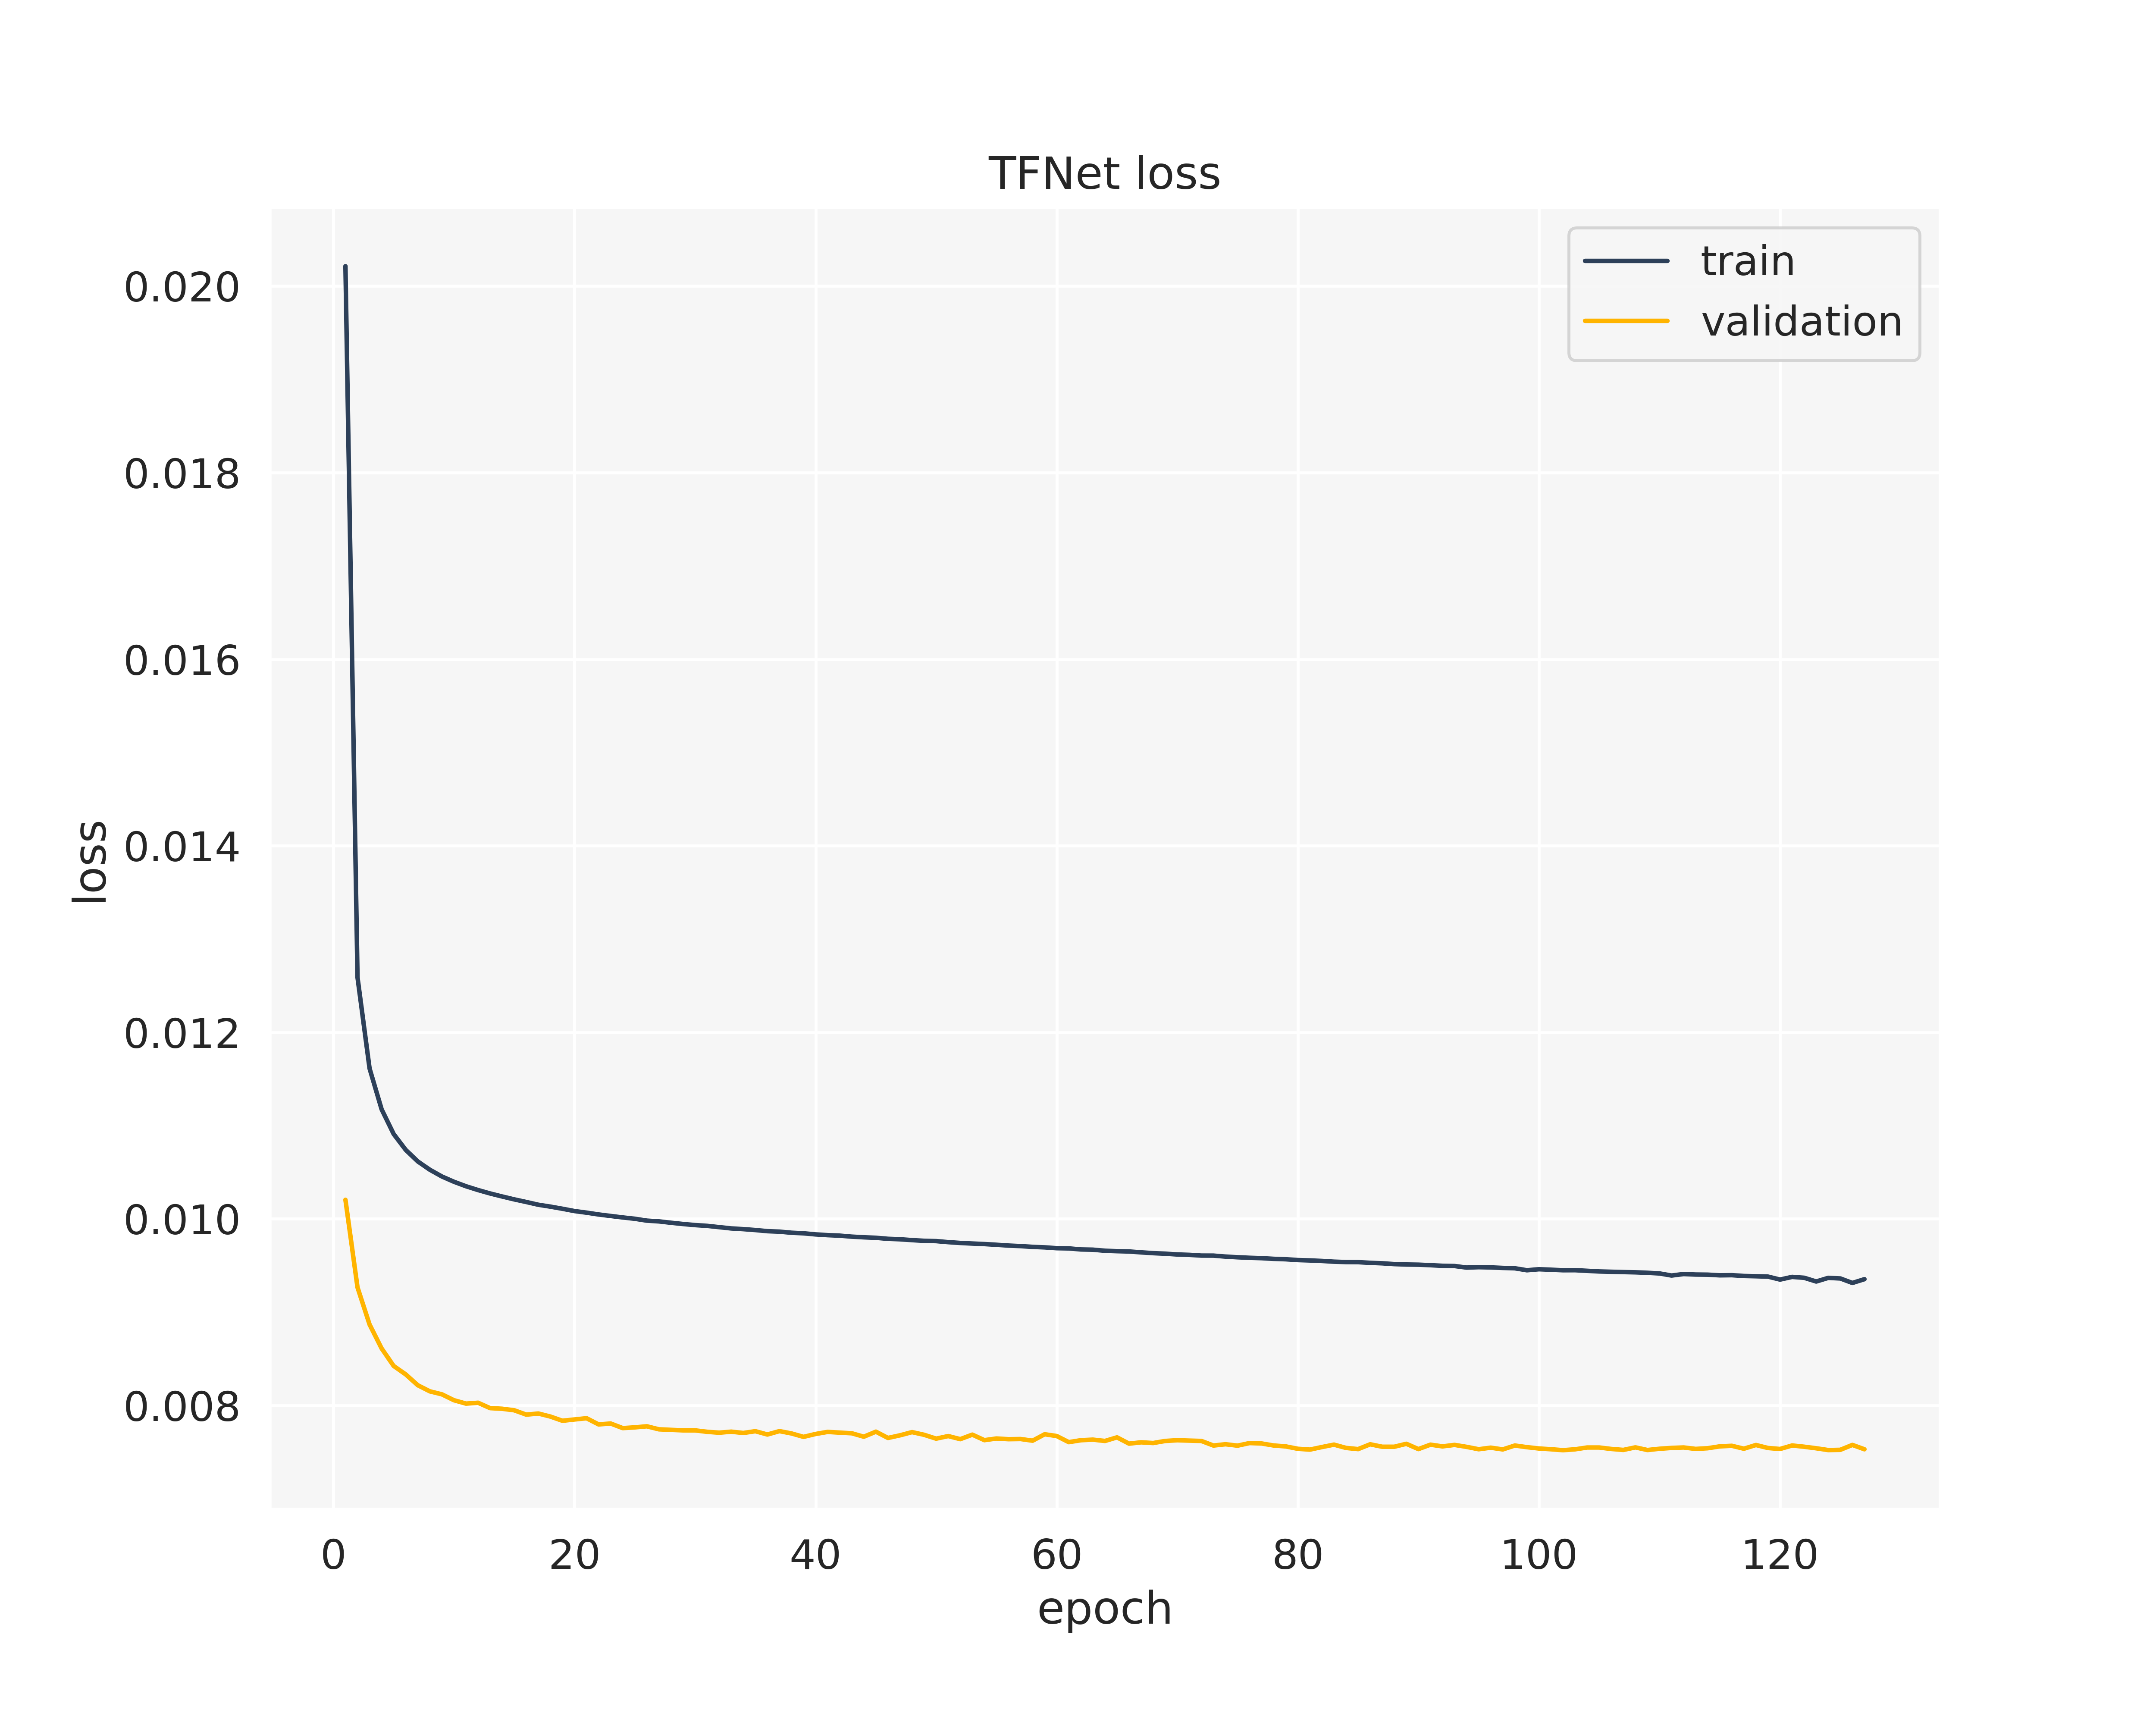
\includegraphics[width=1.05\linewidth]{img/tfnet_loss.png}
		\label{fig:tfnet_loss}
	\end{subfigure}%
	\begin{subfigure}{.5\textwidth}
		\centering
		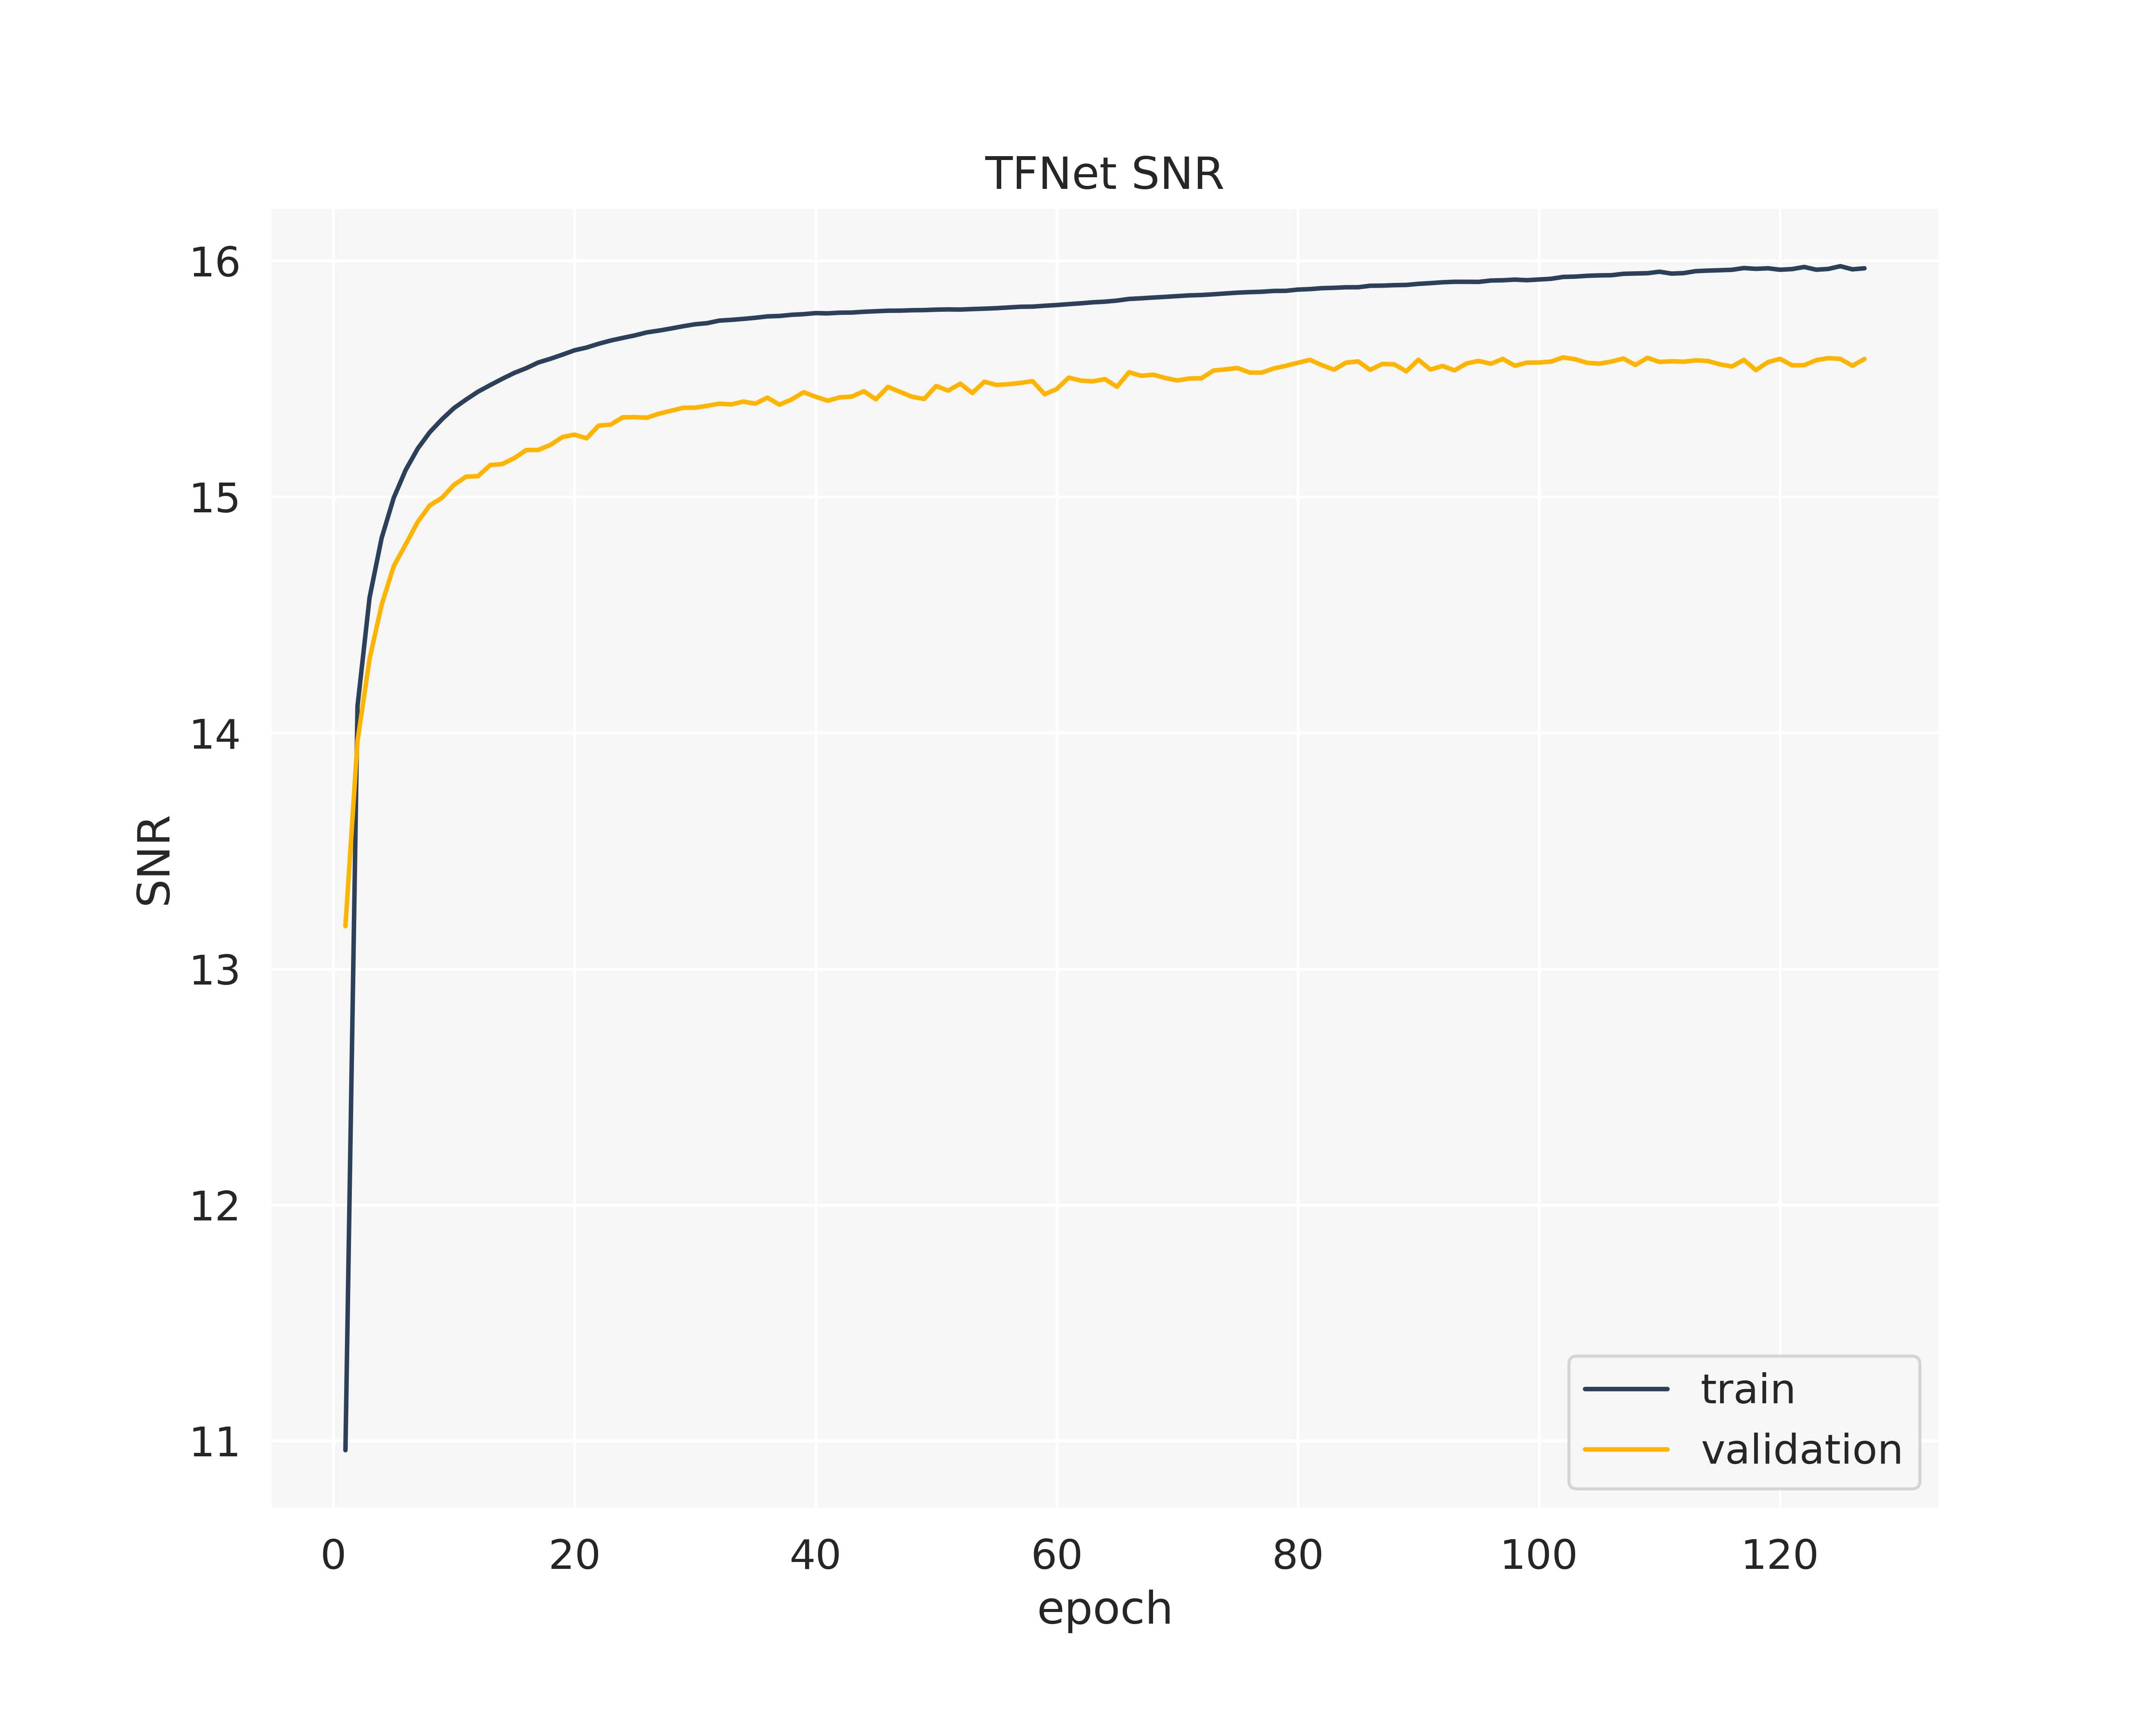
\includegraphics[width=1.05\linewidth]{img/tfnet_snr.png}
		\label{fig:tfnet_snr}
	\end{subfigure}%
	\caption{\gls{tfnet} training curves on both training and validation sets. The model is trained for 127 epochs.}
	\label{fig:tfnet_training_curves}
\end{figure}

\begin{figure}[!htb]
	\begin{subfigure}{.5\textwidth}
		\centering
		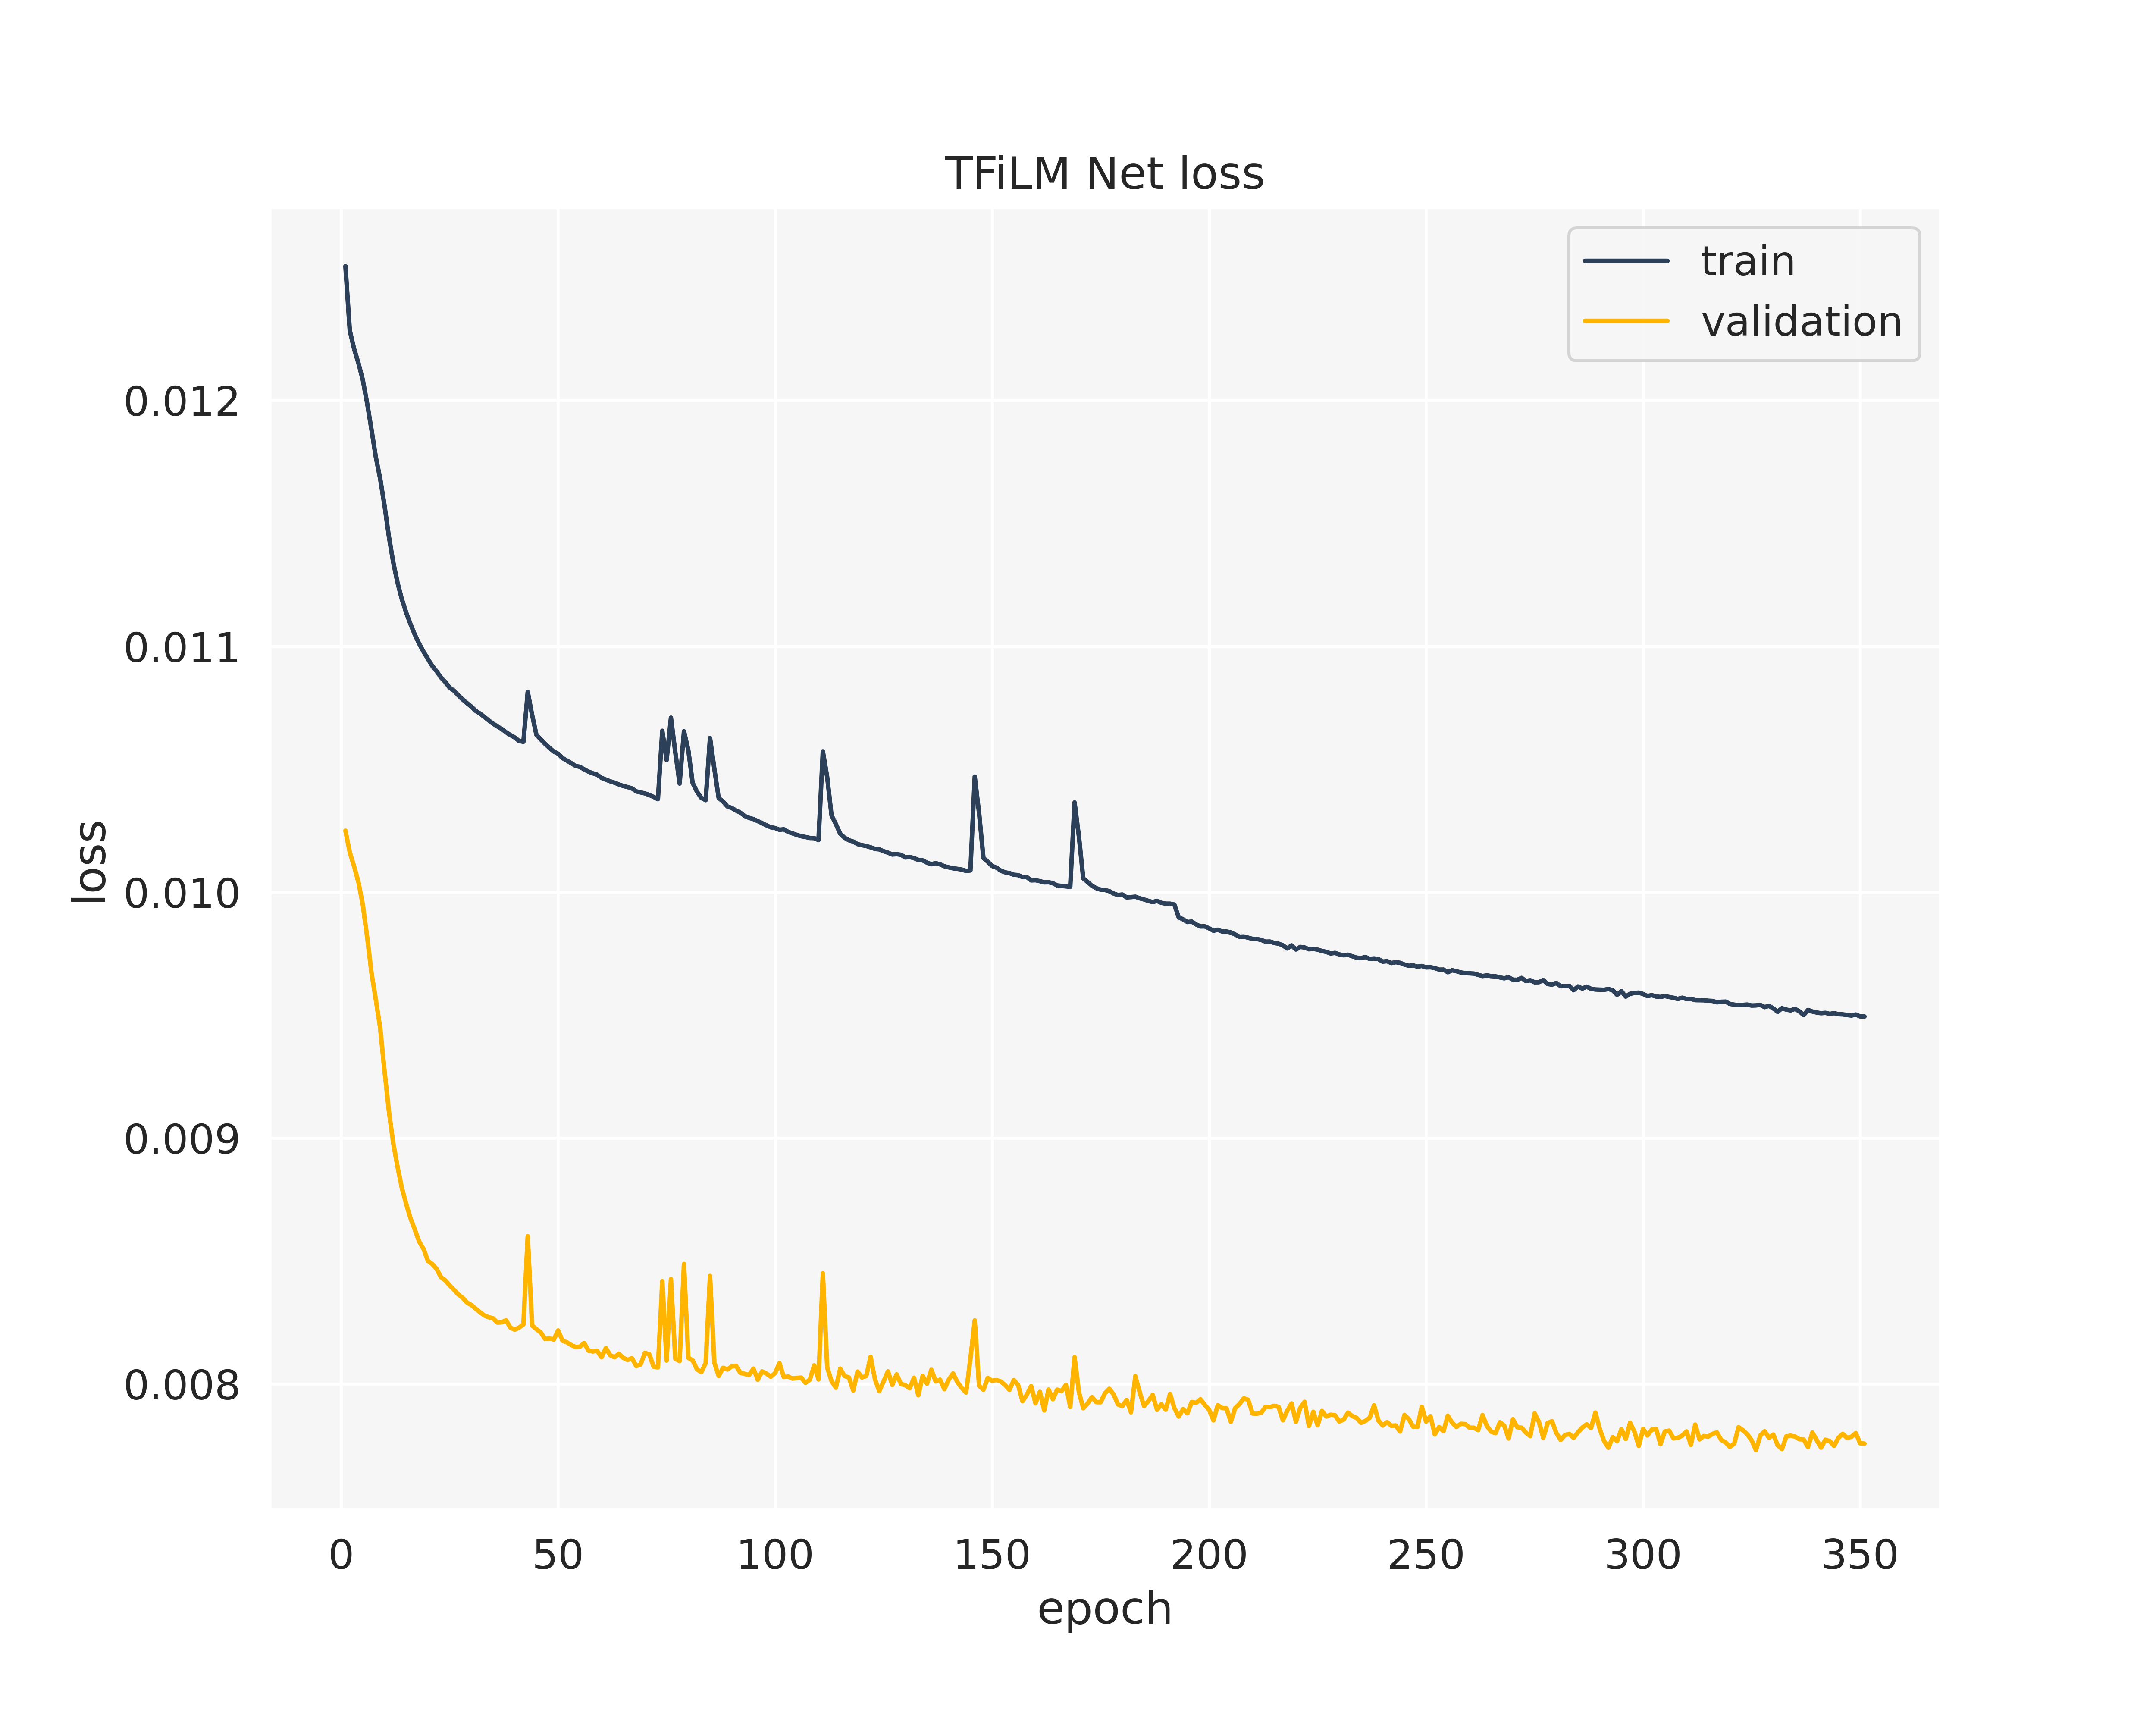
\includegraphics[width=1.05\linewidth]{img/tfilmnet_loss.png}
		\label{fig:tfilmnet_loss}
	\end{subfigure}%
	\begin{subfigure}{.5\textwidth}
		\centering
		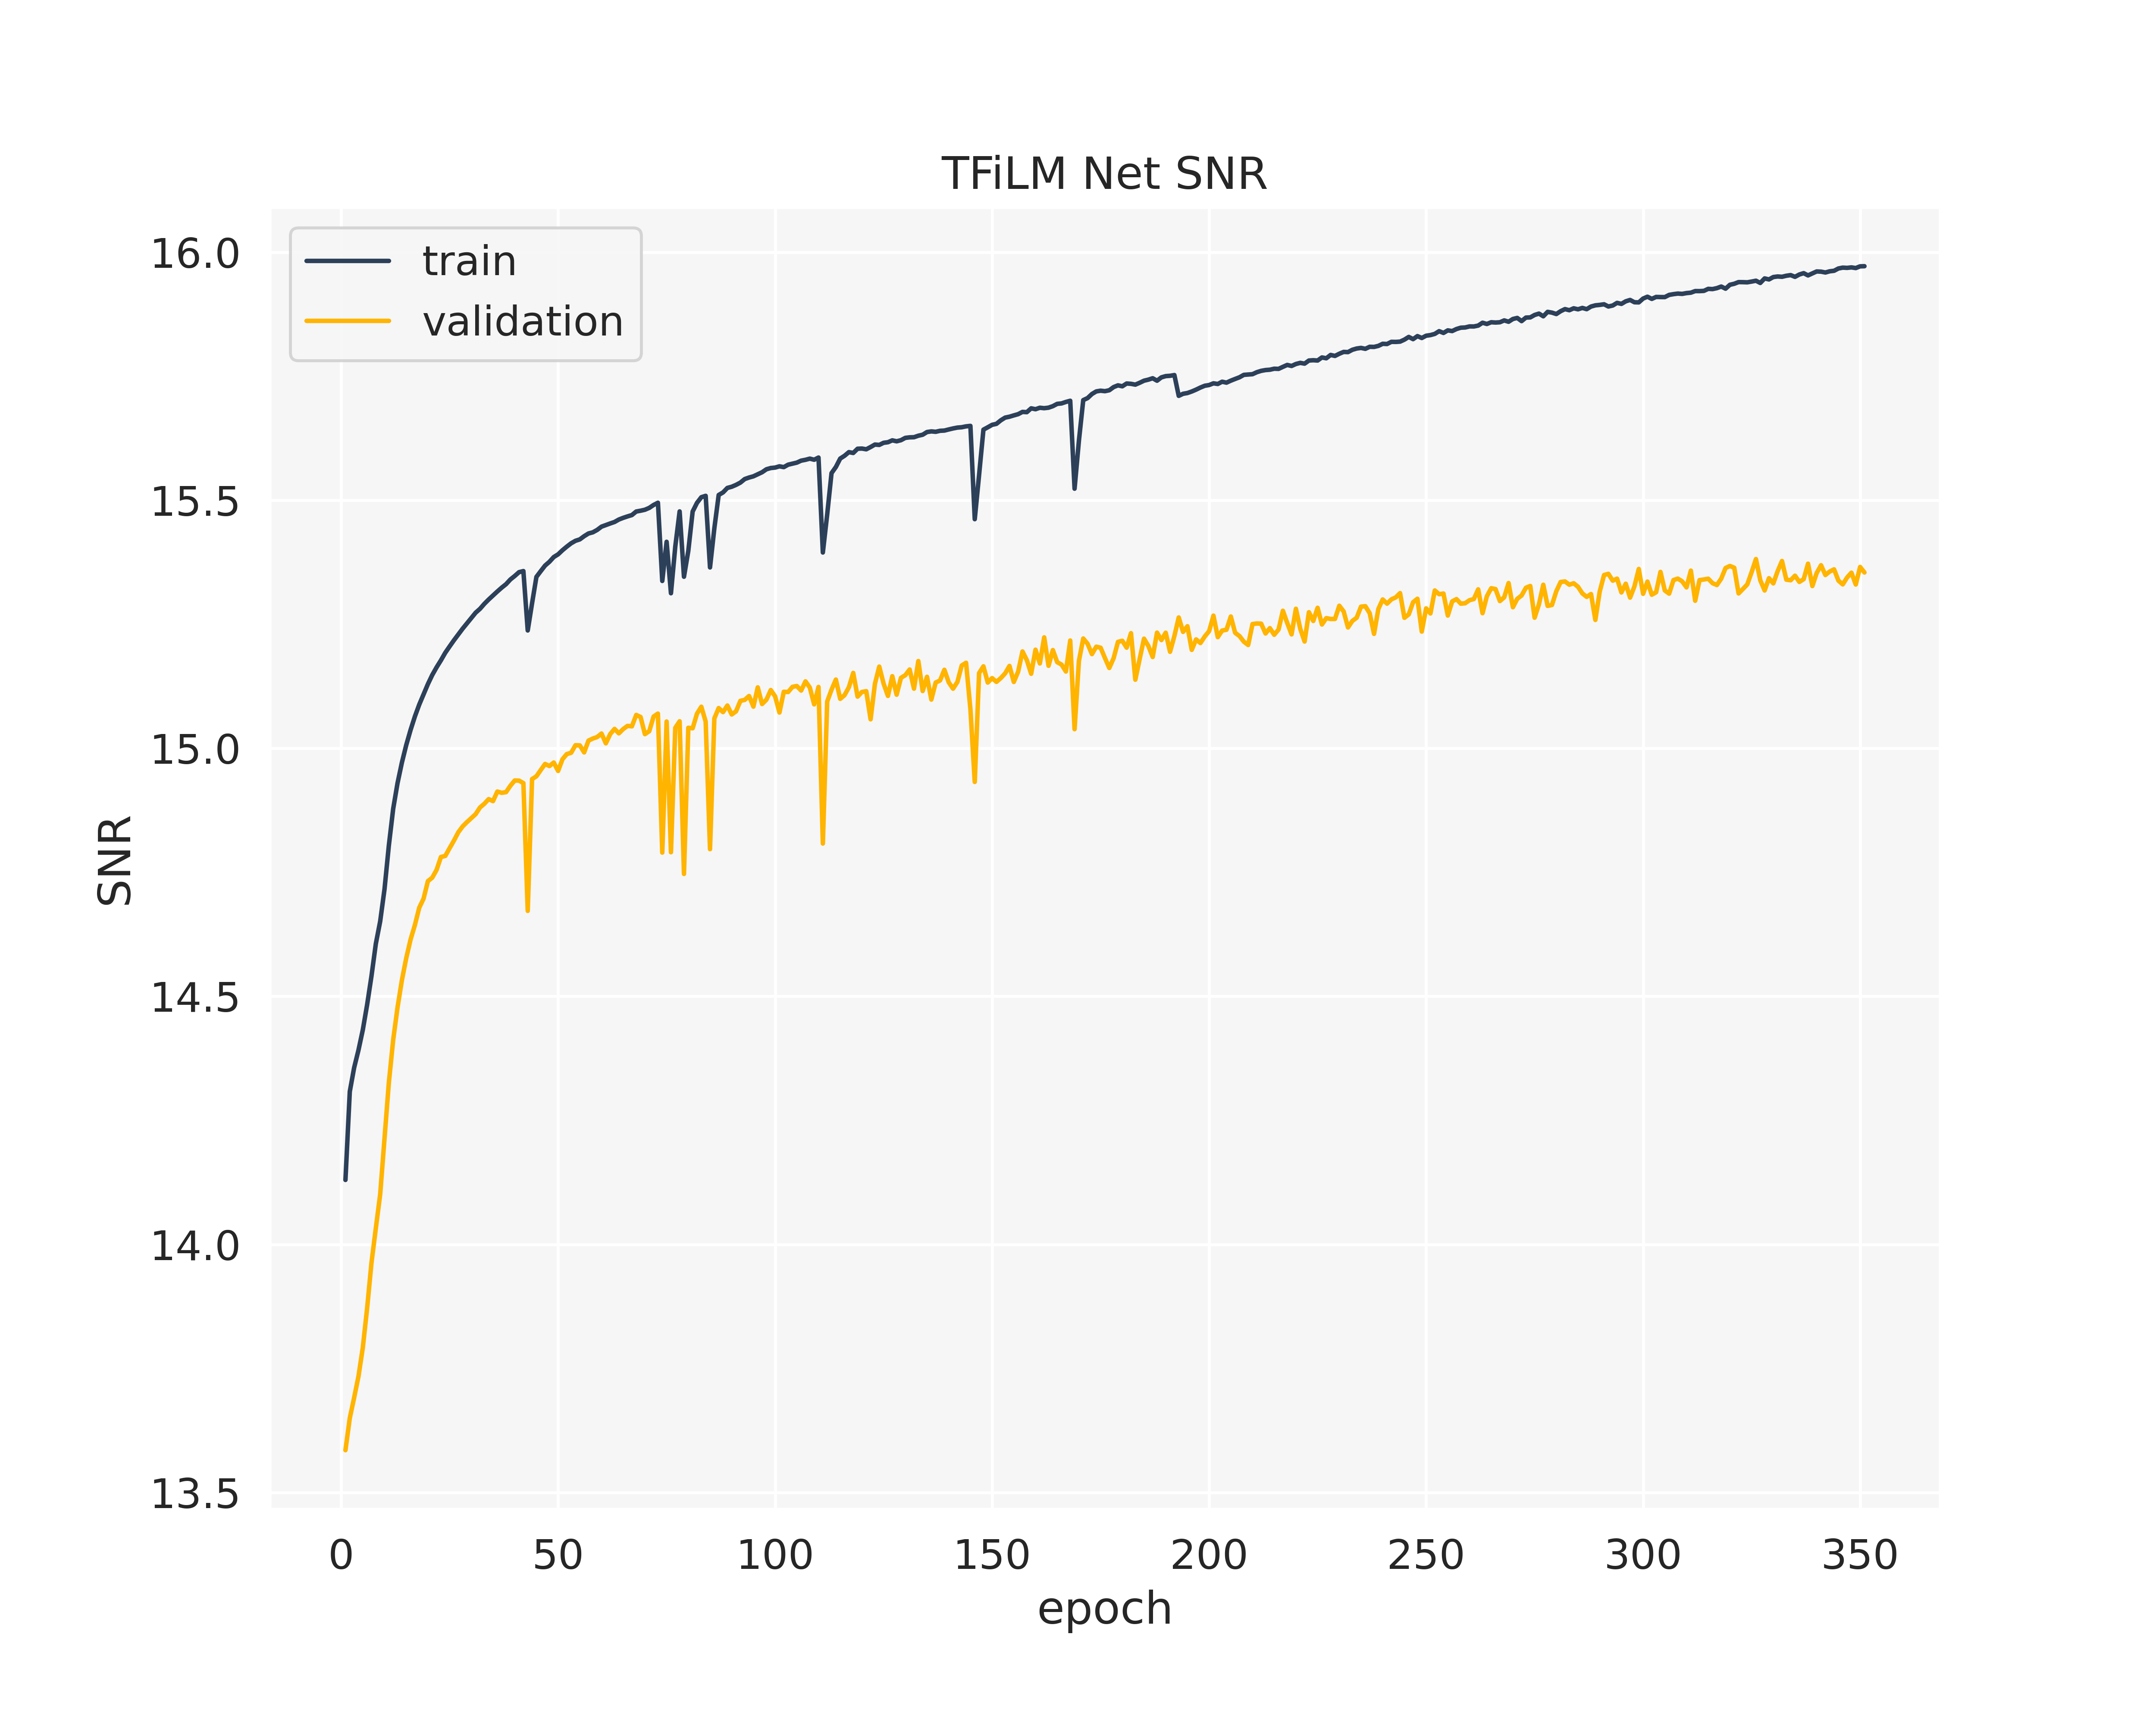
\includegraphics[width=1.05\linewidth]{img/tfilmnet_snr.png}
		\label{fig:tfilmnet_snr}
	\end{subfigure}%
	\caption{\gls{tfilm} Net training curves on both training and validation sets. The model is trained for 351 epochs.}
	\label{fig:tfilmnet_training_curves}
\end{figure}

\begin{figure}[!htb]
	\begin{subfigure}{.5\textwidth}
		\centering
		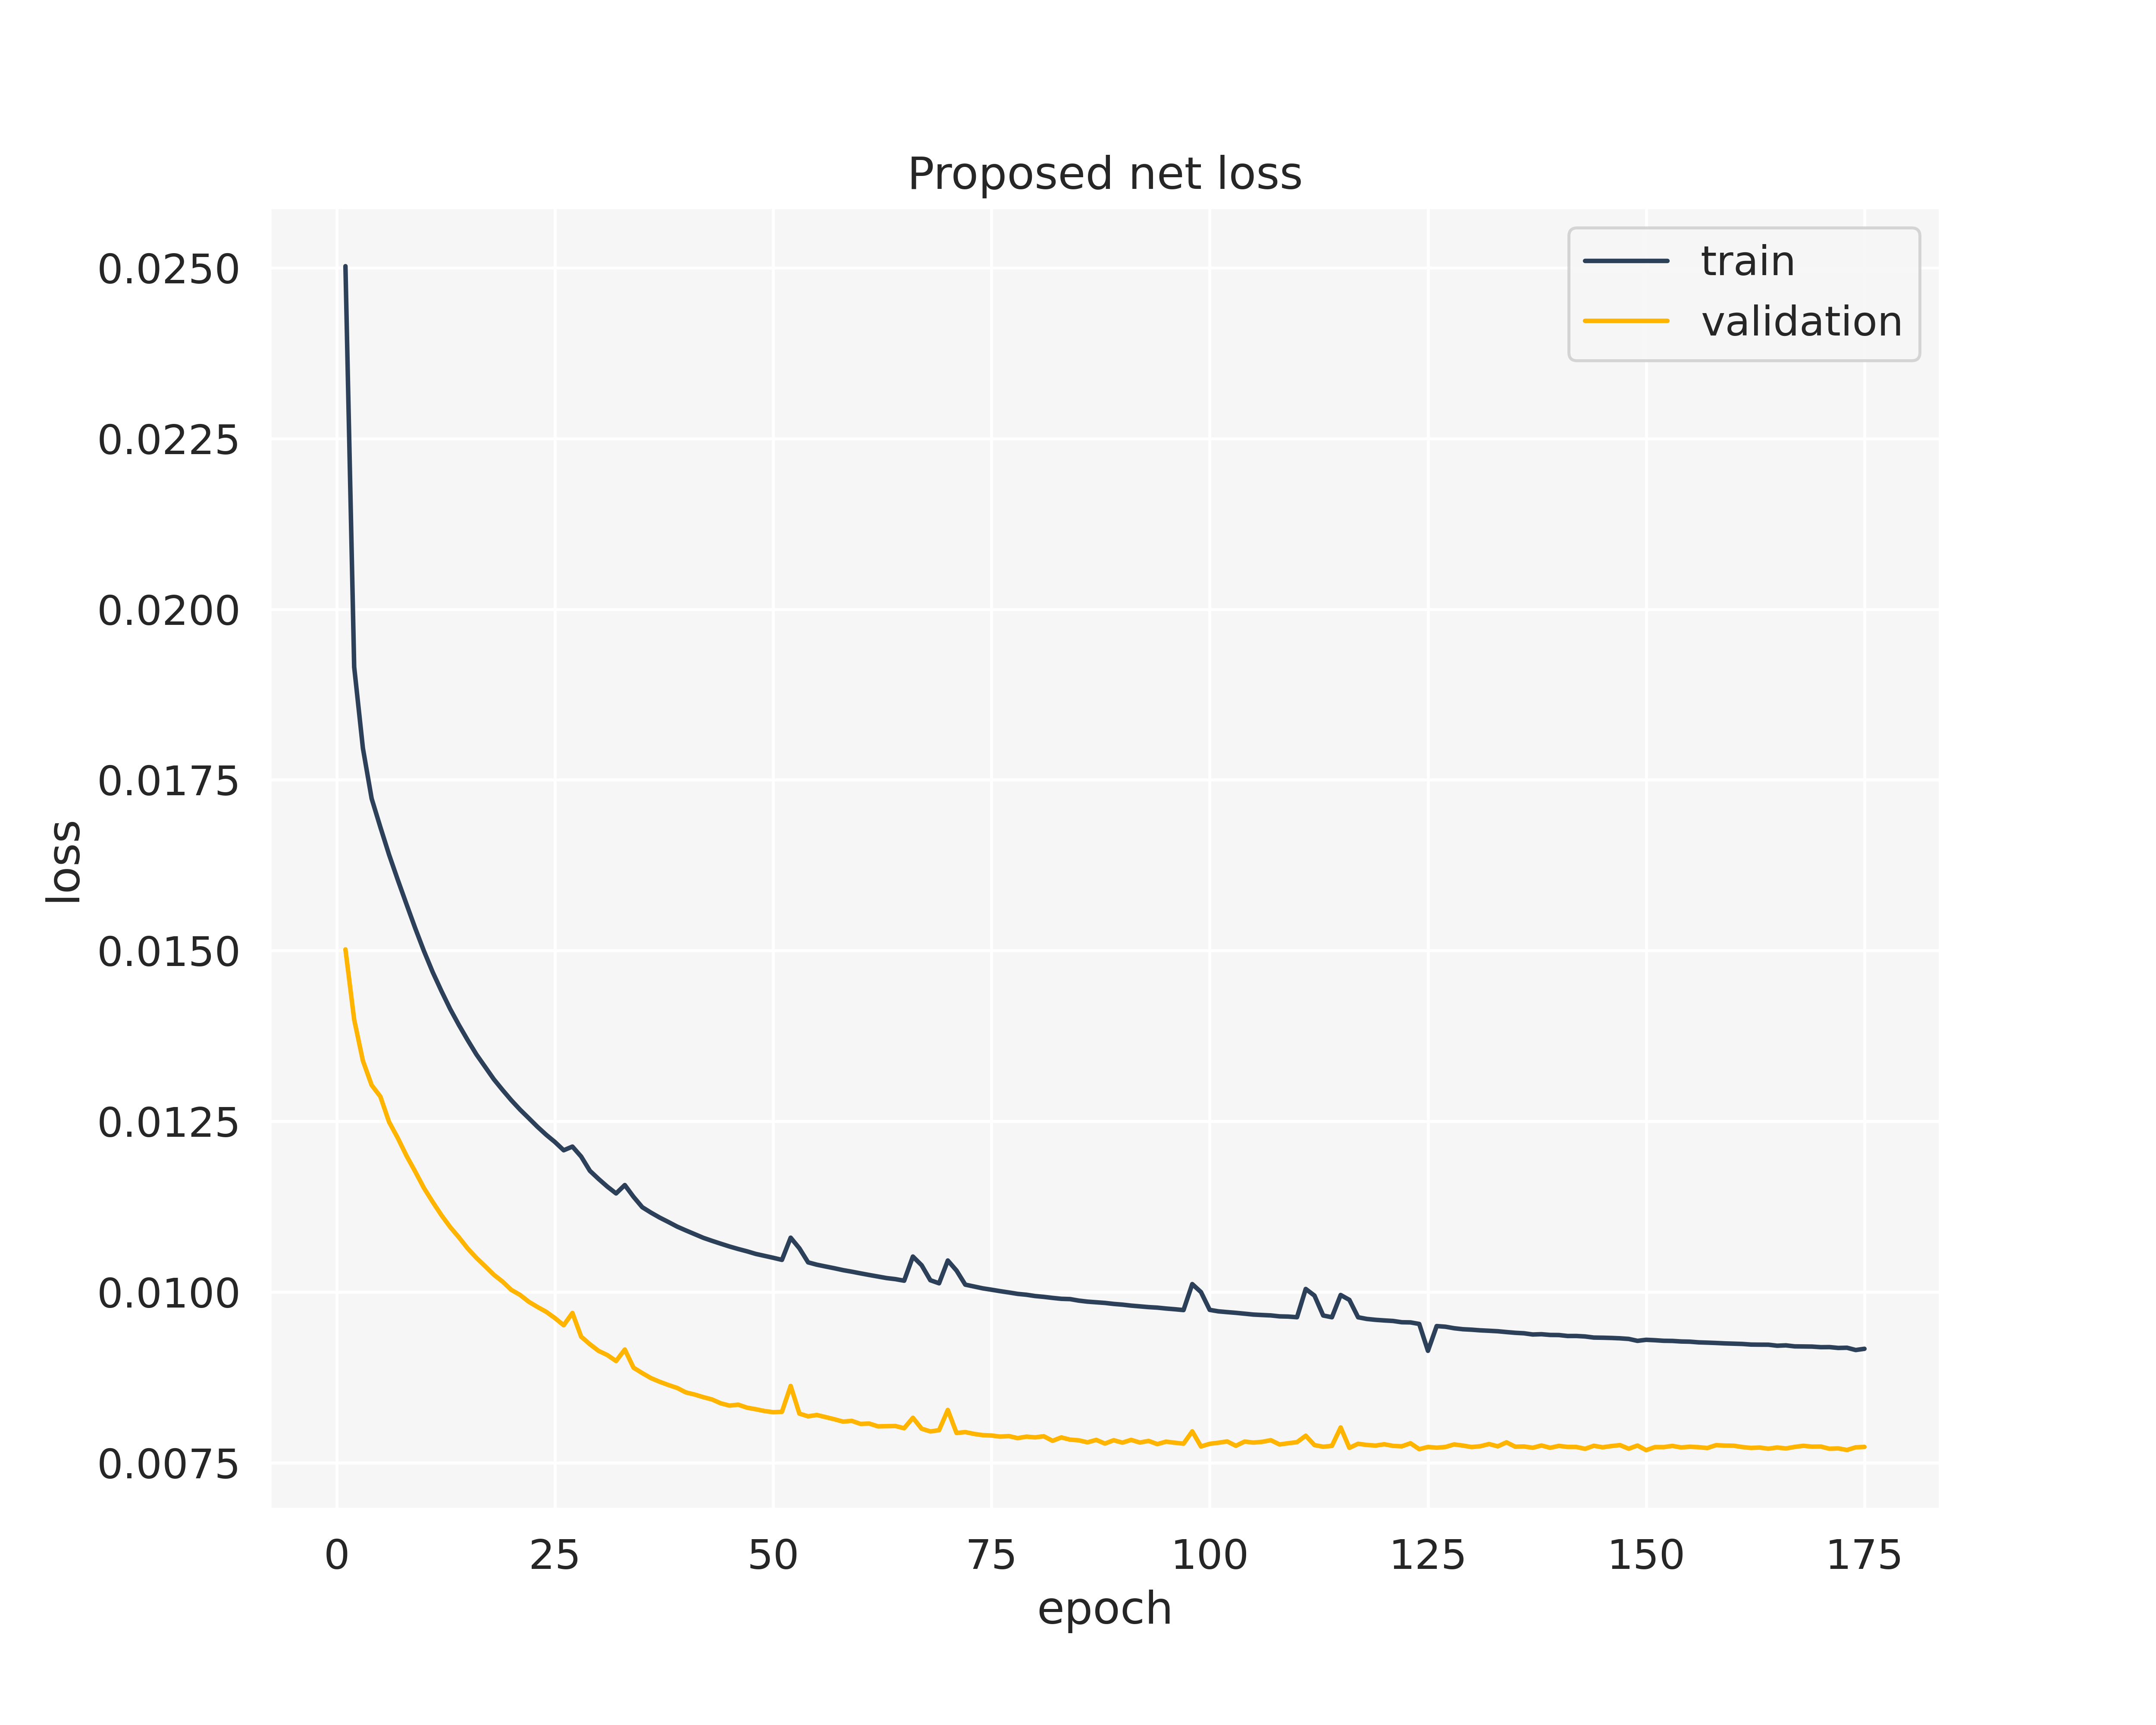
\includegraphics[width=1.05\linewidth]{img/gionet_loss.png}
		\label{fig:gionet_loss}
	\end{subfigure}%
	\begin{subfigure}{.5\textwidth}
		\centering
		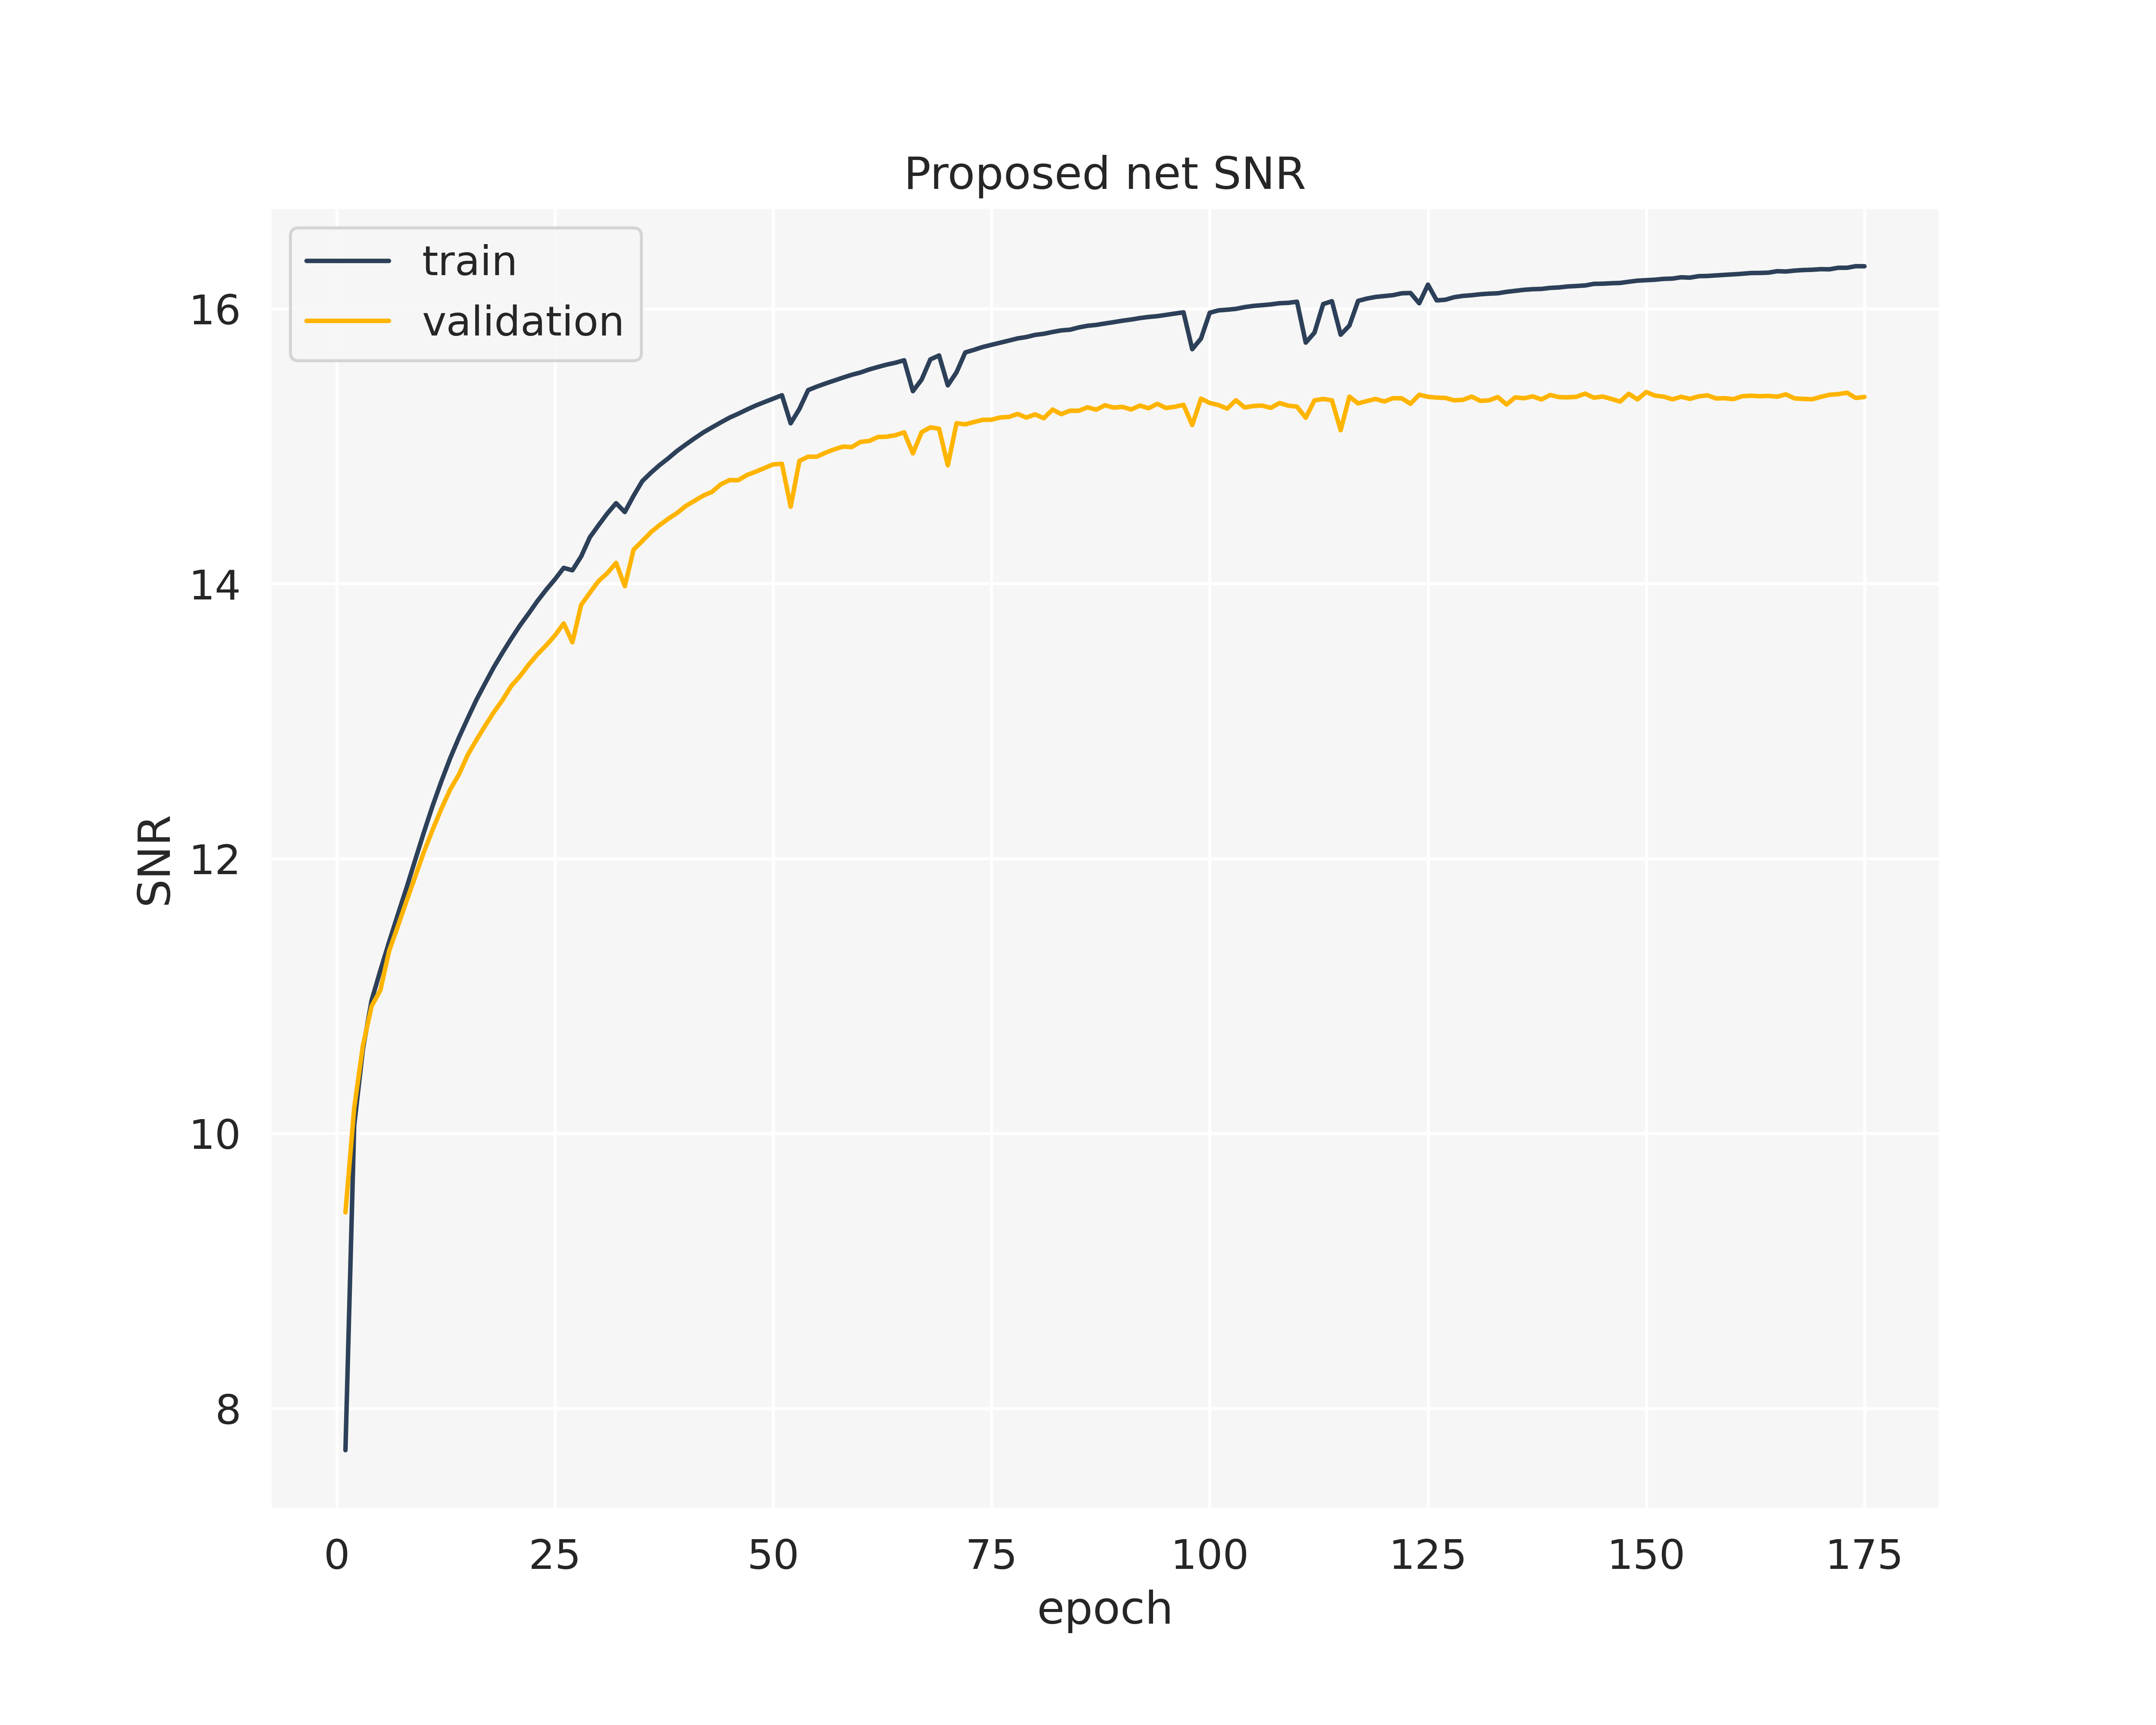
\includegraphics[width=1.05\linewidth]{img/gionet_snr.png}
		\label{fig:gionet_snr}
	\end{subfigure}%
	\caption{Proposed net training curves on both training and validation sets. The model is trained for 175 epochs.}
	\label{fig:proposed_training_curves}
\end{figure}

\noindent We can see that although the loss values in the validation set are better than in the training set, the \gls{snr} value is generally lower. This may be due to the different data distribution in the two sets; in fact, we remind that in the validation set there are more silence audio frames, which instead are filtered from training data.\\
Another relevant aspect is the following: initially, each model is trained on the Multi-Speaker task. Subsequently, Single-Speaker models are obtained through a \textit{fine tuning} operation of the previously trained models. Fine tuning consists in training a pre-trained model on a smaller dataset. More specifically, it is the practice of using pre-trained weights from a model trained on a large dataset (in our case, the \gls{vctk} corpus) as a starting point for a different dataset (\gls{vctk}s). By doing so, we exploit a greater power of generalization (the one of Multi-Speaker models) instead of starting from scratch. \\
It is worth stressing that the optimizer, the number of training steps, the learning rate, and the other hyperparameters are kept the same for both Single-Speaker and Multi-Speaker regimes. Consequently, this results in a larger number of epochs for the Single-Speaker task since \gls{vctk}s is significantly smaller than \gls{vctk}. \\
Finally, we mention that in the Multi-Speaker we select as the final model configuration the one which corresponds to the last validation set improvement on either the loss or the \gls{snr} values. On the other hand, in the Single-Speaker task, since there is no validation set, we simply take the model weights at the last epoch.

\subsection{Evaluation Methods} \label{eval_methods}
In this section the metrics used to evaluate the models introduced in Chapter \ref{chap:methods} are presented. We use two standard metrics used in the audio \gls{sr} literature such as \gls{snr} and \gls{lsd} \cite{gray1976distance}. While the former takes into account a weighted difference between the model signal reconstruction and the ground-truth data in the time domain, the latter measures the reconstruction quality in the frequency domain. \\
More specifically, \gls{snr} is the ratio, usually expressed on a logarithmic scale in decibels, between the signal power level and the noise power level. Formally, given a reference signal $y$ and an approximation $\hat{y}$, the Signal-to-Noise ratio \gls{snr} is defined as:

\begin{align}\label{eq:snr}
	\operatorname{SNR}(\hat{y}, y)=10 \log\frac{\|y\|_{2}^{2}}{\|\hat{y}-y\|_{2}^{2}}
\end{align}

\noindent As for \gls{lsd}, a formal definition is as follows. Let $X$ and $\hat{X}$ be the log-spectral power magnitudes of, respectively, the reference signal $y$ and its approximation $\hat{y}$. These are defined as $X = \log |S|^2$, where $S$ is the \gls{stft} of the signal. Then, the \gls{lsd} can be calculated as: 

\begin{align}\label{eq:lsd}
	\operatorname{LSD}(\hat{y}, y)=\frac{1}{L} \sum_{\ell=1}^{L} \sqrt{\frac{1}{K} \sum_{k=1}^{K}(X(\ell, k)-\hat{X}(\ell, k))^{2}}
\end{align}

\noindent where $\ell$ denotes the index of short windowed frames of the audio and $k$ denotes frequencies; in our experiments (as well as in \cite{kuleshov2017audio}, \cite{lim2018time}, \cite{birnbaum2019temporal}) we use frames of length 2048. \\
Furthermore, we investigate the effect of each model in the context of a wider system, which also includes a model of \gls{stt}: as said in Chapter \ref{chap:intro}, a \gls{bwe} algorithm has the potential to help in better performing the speech-to-text conversion task by improving the quality of input recordings. \\
Our objective is to investigate whether or not the results of a \gls{stt} system obtained on a \gls{lr} input signal improve after a \gls{sr} operation is performed. Thus, we use one of the state-of-the-art open-source \gls{stt} engines, i.e. \textit{Deep Speech} \cite{hannun2014deep} to process the recordings and obtain their textual transcription. \\
In order to quantify the word level mismatch between real and predicted textual transcriptions we use a standard evaluation metric such as \gls{wer}. According to \cite{morris2004and}, we can define \gls{wer} as the proportion of word errors to words processed. More specifically, let denote with $H, S, D, I$ the total number of word hits, substitutions, deletions and insertions (see Fig. \ref{fig:wer_letters}). Then the \gls{wer} can be calculated as:
\begin{align}\label{eq:wer}
	\operatorname{WER} =\frac{S + D + I}{H + S + D}
\end{align}

\begin{figure}[!htb]
	\begin{center}
		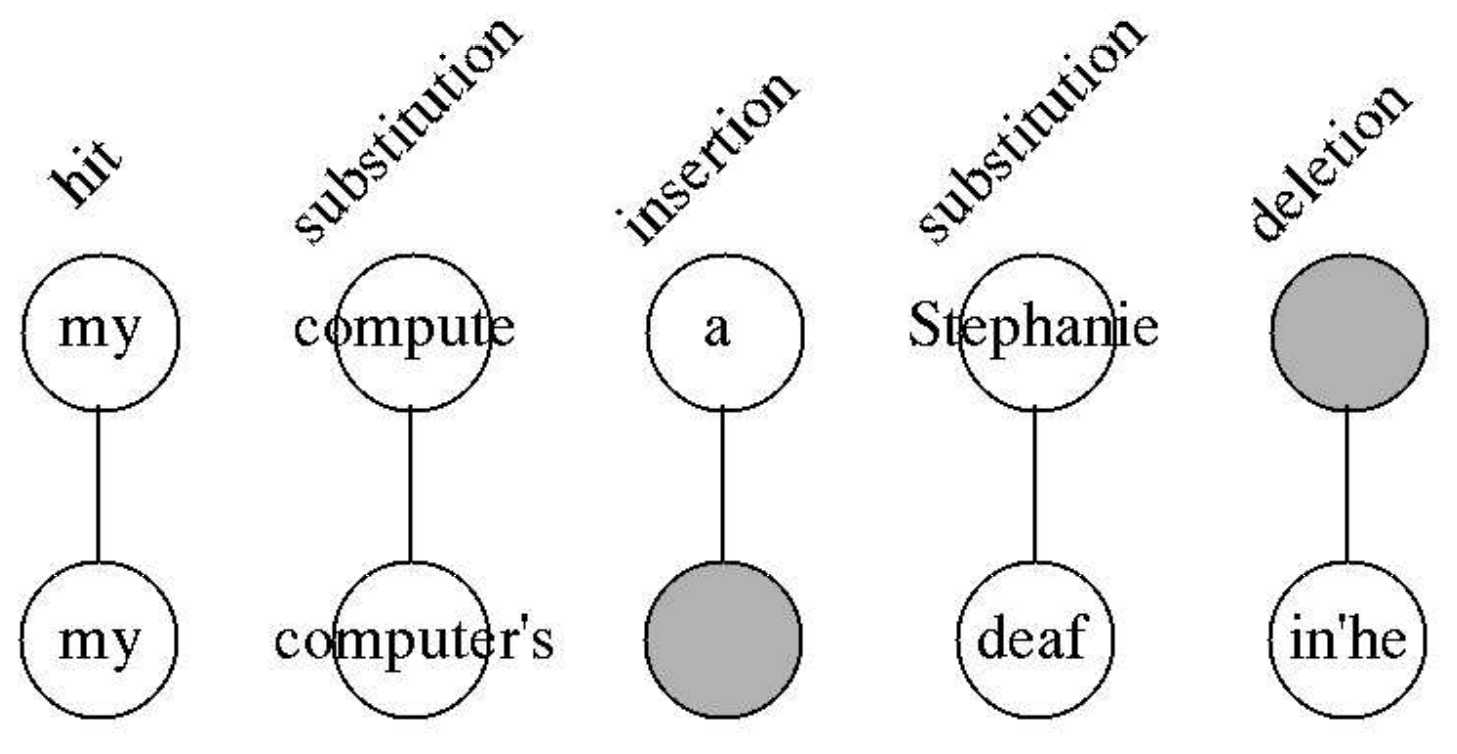
\includegraphics[scale=0.4]{img/wer_letters.png}
		\caption{Example of $H, S, D, I$ classification on the input words “my computer’s deaf in’he?”. From \cite{morris2004and}.}
		\label{fig:wer_letters}
	\end{center}
\end{figure}

\noindent An important aspect is that it is necessary to apply some appropriate pre-processing steps on both the predicted and the ground-truth transcription text. In particular, these operations consists in removing leading and trailing spaces, reducing text to lower case, expanding all contractions and removing punctuation. \\
Finally, it is important to highlight that, while \gls{snr} and \gls{lsd} are calculated on the test set patches, \gls{wer} is calculated on the test set full recordings. 

\section{Results} \label{results}
This section describes and discusses the main results achieved in the reported experiments in order to establish the best model architecture. We provide results on both the Multi-Speaker and the Single-Speaker regimes in order to investigate if the proposed algorithm allows improving the audio \gls{sr} task. \\
Our method is compared to three baselines: a cubic B-spline — which corresponds to the upsampling criteria used in all model pipelines (Figures \ref{fig:tfnet_pipeline}, \ref{fig:tfilm_pipeline}, \ref{fig:proposed_pipeline}) - \gls{tfnet} and \gls{tfilm} Net. \\
We remind that a higher \gls{snr} is better, a lower \gls{lsd} is better and a lower \gls{wer} is better. \\
The results of our experiments over the training set are summarized in tables \ref{tab:s_speaker_tr} and \ref{tab:m_speaker_tr}. As we can see, our solution achieves the best \gls{snr} and \gls{lsd} values on both tasks. However, high training performance are not, in general, always associated with high generalization results. Furthermore, we remind that, in our setting, the training set data distribution is not highly representative of the problem as we filter silence audio frames. \\
Therefore, we use a validation set, which allows to have a more accurate estimate of the generalization power of the models during the training phase. Validation set results can be seen in Table \ref{tab:m_speaker_val}; the proposed model outperforms the other models on \gls{lsd} score, while its \gls{snr} is not as good as the \gls{tfnet} system one. \\

\begin{table}[!htb]
	\begin{center}
		\begin{tabular}{@{}ccccc@{}}
			\toprule
			\multicolumn{5}{c}{\textbf{\begin{tabular}[c]{@{}c@{}}Single-Speaker\\ \textit{\scriptsize{Training Set}}\end{tabular}}}  \\ \midrule
			Obj. & Spline & TFNet & TFiLM Net & Proposed \\ \midrule
			SNR & 14.74 & 16.93 & 16.71 & \textbf{17.33} \\ \midrule
			LSD & 5.64 & 3.44 & 3.93 & \textbf{3.24} \\ \bottomrule
		\end{tabular}
		\caption{Evaluation of \gls{bwe} methods (in \gls{db}) on the Single-Speaker task over the training set in terms of \gls{snr} and \gls{lsd}. A higher \gls{snr} is better and a lower \gls{lsd} is better.}
		\label{tab:s_speaker_tr}
	\end{center}
\end{table}

\begin{table}[!htb]
	\begin{center}
		\begin{tabular}{@{}ccccc@{}}
			\toprule
			\multicolumn{5}{c}{\textbf{\begin{tabular}[c]{@{}c@{}}Multi-Speaker\\ \textit{\scriptsize{Training Set}}\end{tabular}}}  \\ \midrule
			Obj. & Spline & TFNet & TFiLM Net & Proposed \\ \midrule
			SNR & 14.29 & 15.97 & 15.96 & \textbf{16.21} \\ \midrule
			LSD & 6.29 & 3.69 & 4.25 & \textbf{3.37} \\ \bottomrule
		\end{tabular}
		\caption{Evaluation of \gls{bwe} methods (in \gls{db}) on the Multi-Speaker task over the training set in terms of \gls{snr} and \gls{lsd}. A higher \gls{snr} is better and a lower \gls{lsd} is better.}
		\label{tab:m_speaker_tr}
	\end{center}
\end{table}

\begin{table}[!htb]
	\begin{center}
		\begin{tabular}{@{}ccccc@{}}
			\toprule
			\multicolumn{5}{c}{\textbf{\begin{tabular}[c]{@{}c@{}}Multi-Speaker\\ \textit{\scriptsize{Validation Set}}\end{tabular}}}  \\ \midrule
			Obj. & Spline & TFNet & TFiLM Net & Proposed \\ \midrule
			SNR & 13.60 & \textbf{15.57} & 15.35 & 15.34 \\ \midrule
			LSD & 5.97 & 3.57 & 4.14 & \textbf{3.31} \\ \bottomrule
		\end{tabular}
		\caption{Evaluation of \gls{bwe} methods (in \gls{db}) on the Multi-Speaker task over the validation set in terms of \gls{snr} and \gls{lsd}. A higher \gls{snr} is better and a lower \gls{lsd} is better.}
		\label{tab:m_speaker_val}
	\end{center}
\end{table}

\noindent At this point, we can examine the extent to which the models generalize across the test set. The results of \gls{snr} in Figure \ref{fig:snr} show that \gls{tfnet} approach is the one which achieves the best values on both tasks. As for the other two methods, they achieve similar performance. Furthermore, we can observe that each model exceeds the spline baseline about more than 1\gls{db}. \\
As for \gls{lsd} scores, we can see from Figure \ref{fig:lsd} that our system shows an improvement of 0.1 - 2.2 \gls{db} over the baseline methods on the Single-Speaker task and even of 0.3 - 2.3 \gls{db} on the Multi-Speaker problem. From an intuitive perspective, we can say that, in our model, the spectral distortions of the predicted speech from the clean speech is less significant at high-frequencies. \\
These two metrics reflect the potential of the models to help the Deep Speech engine in better performing the \gls{stt} conversion. In fact, as we can see from Figure \ref{fig:wer}, the results of \gls{wer} show that the two best models are again \gls{tfnet} and the proposed one. In particular, we can see that our approach outperforms by approximately 0.05 percentage points the \gls{tfnet} system, by $\approx$ 0.08 percentage points the \gls{tfilm} Net and by $\approx$ 0.12 percentage points the spline baseline. Although these results are quite far from the \gls{wer} obtained on original recordings (which is an estimate of the real potential of the Deep Speech engine), the improvements brought by the audio \gls{sr} models are remarkable when compared to splines.\\
\begin{figure}[H]
	\begin{center}
		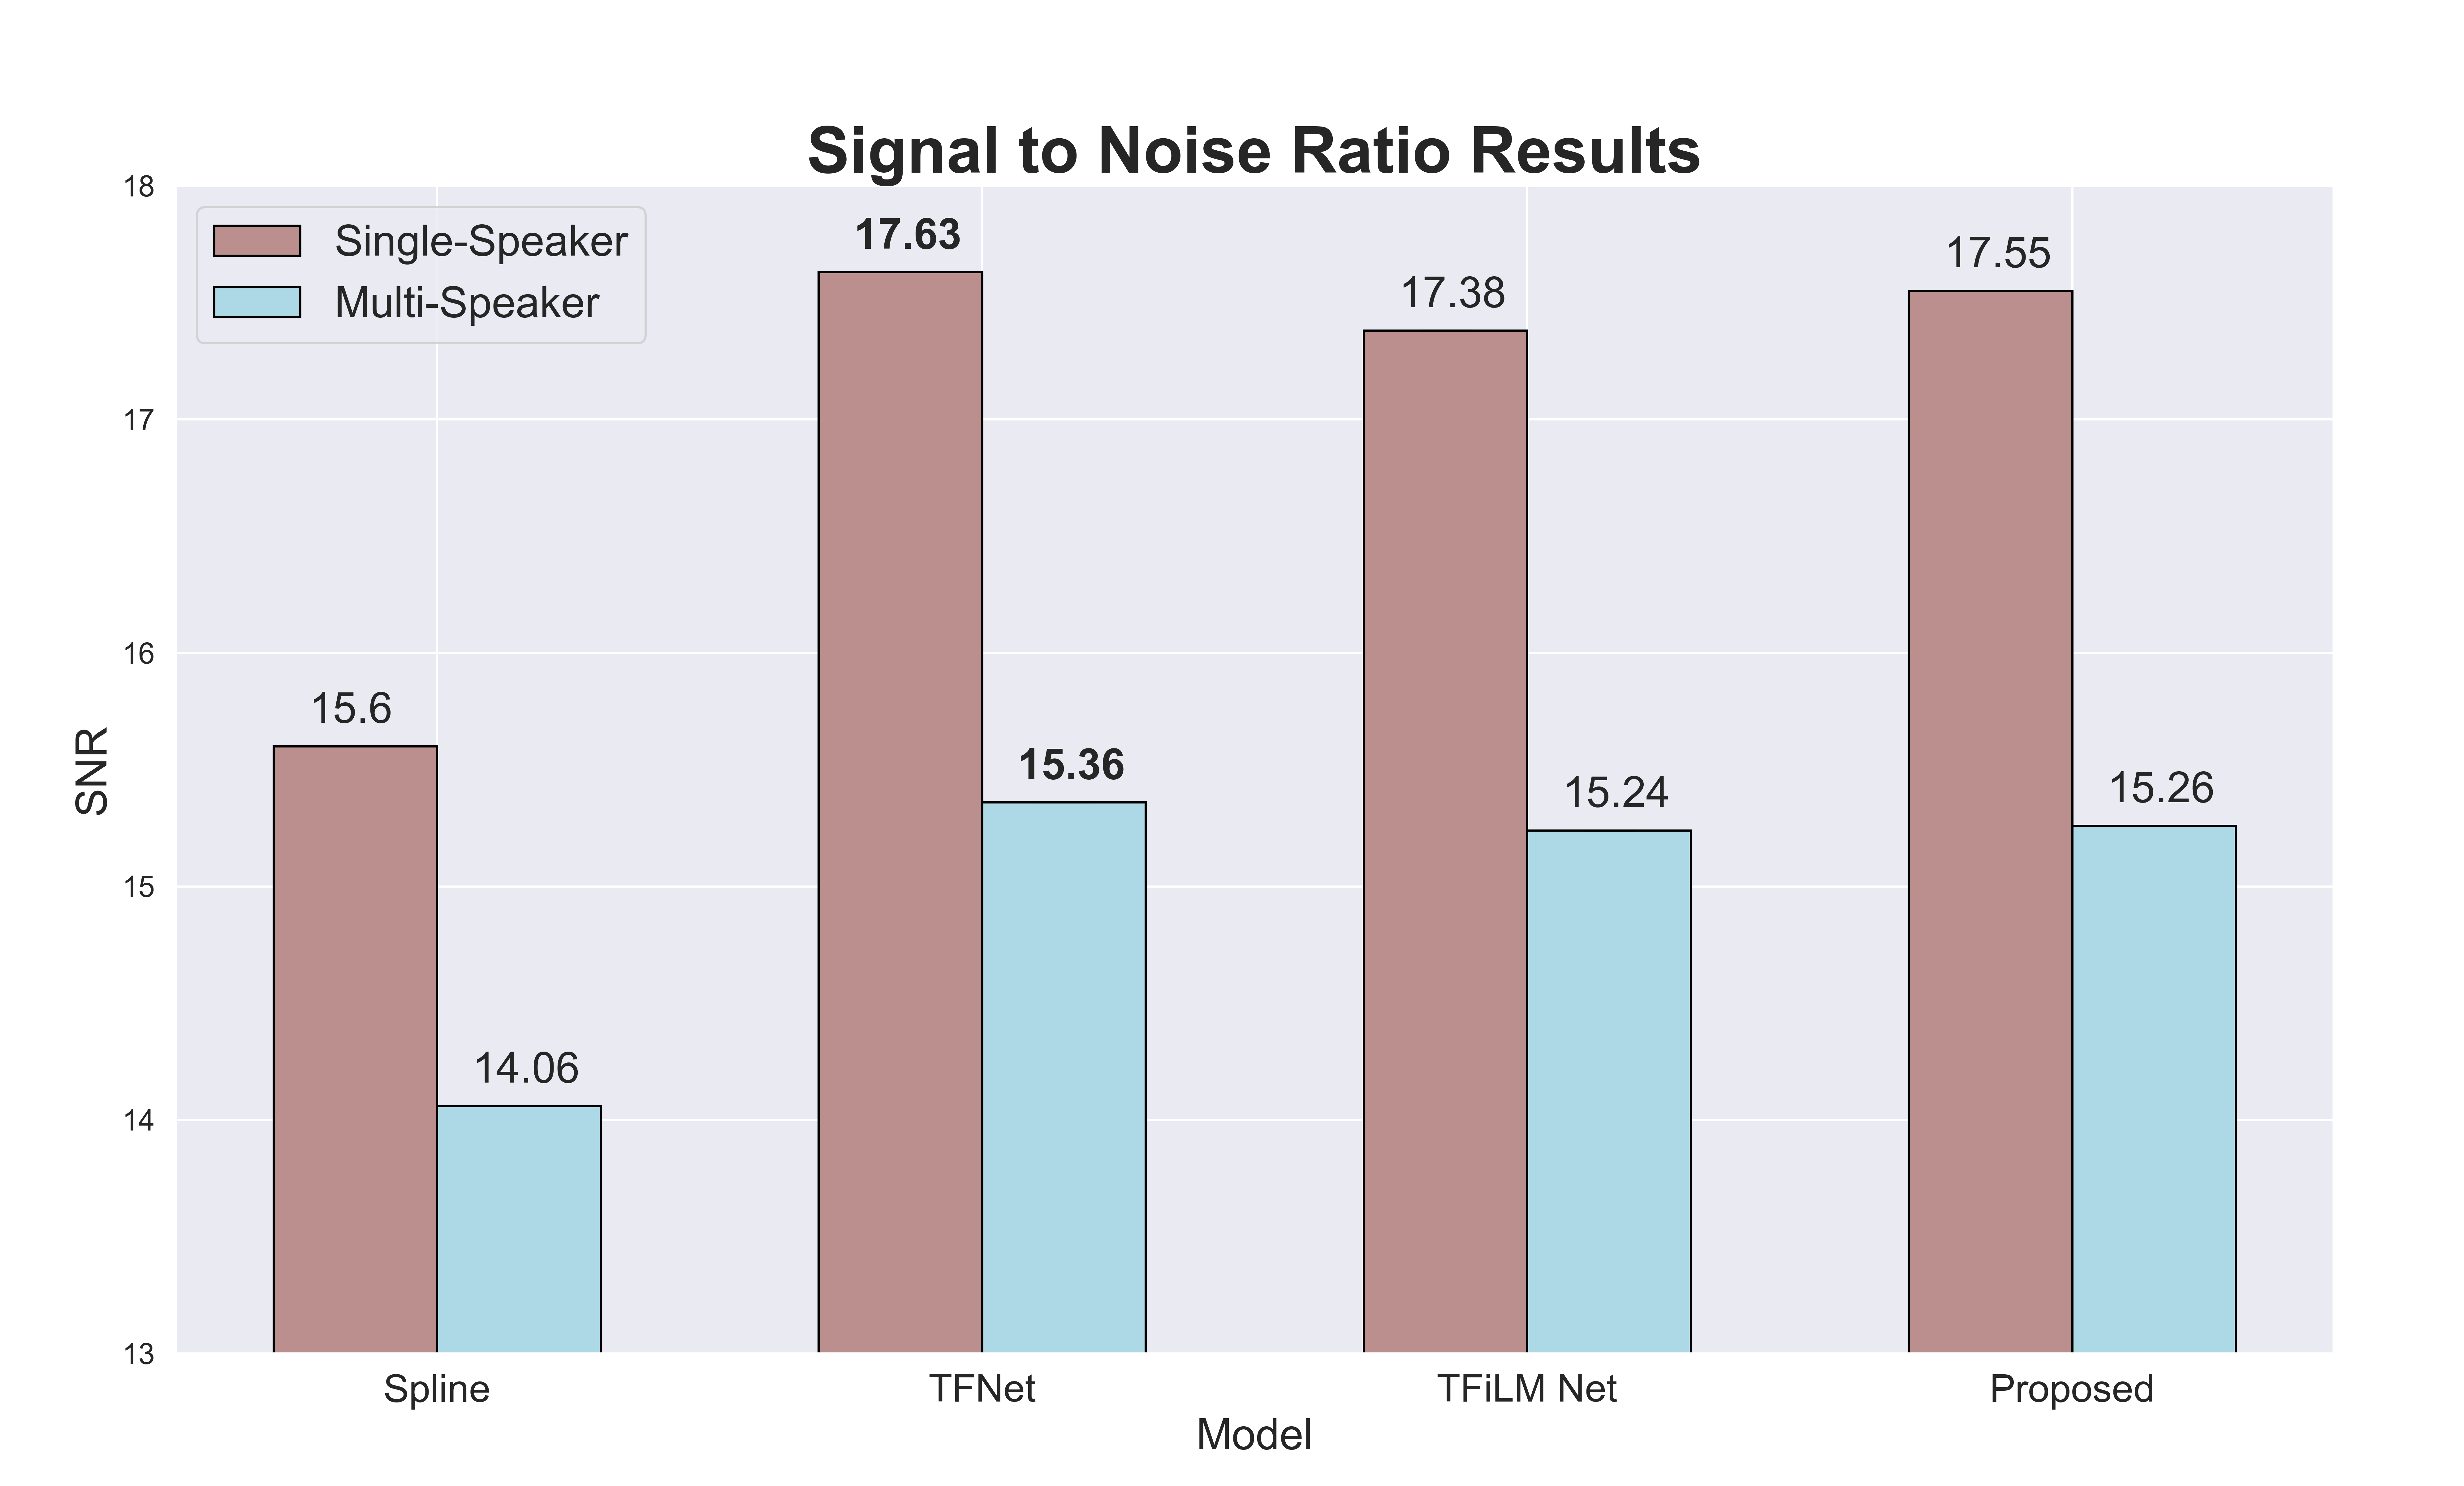
\includegraphics[scale=0.4]{img/snr_results.png}
		\caption{SNR results (in \gls{db}) on Test Set for both Single-Speaker and Multi-Speaker tasks. Higher is better.}
		\label{fig:snr}
	\end{center}
\end{figure}

\begin{figure}[!htb]
	\begin{center}
		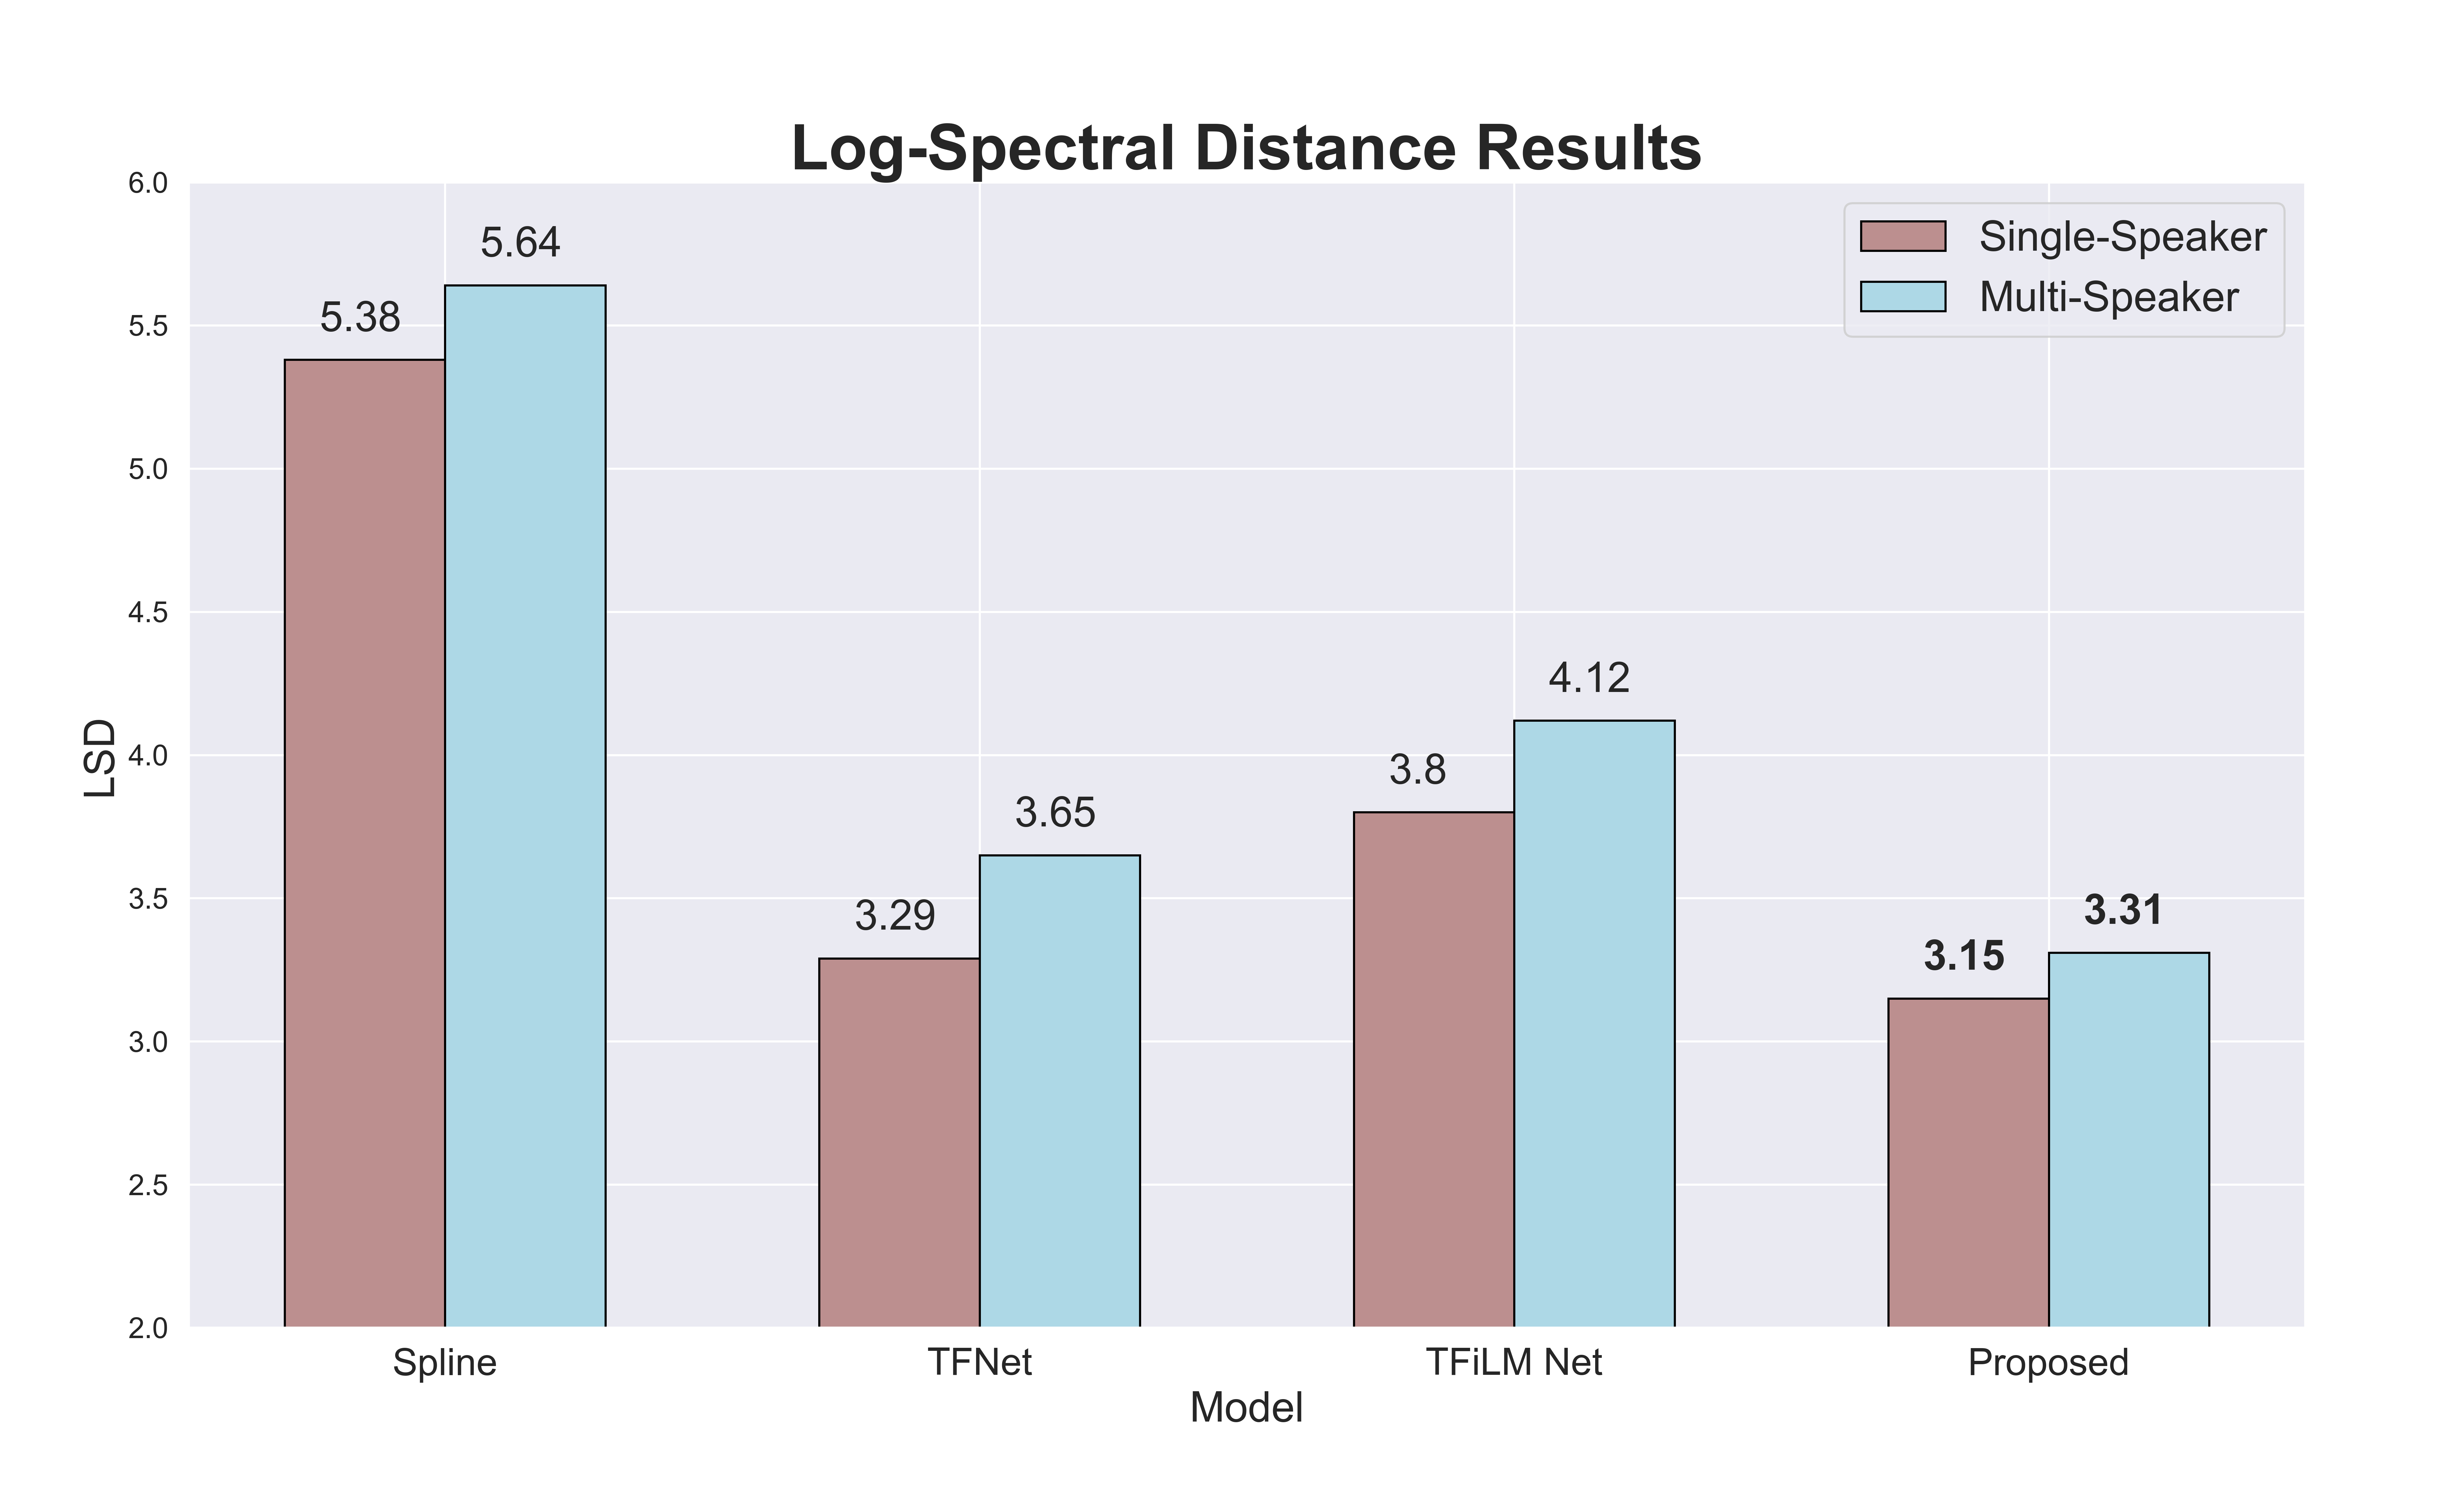
\includegraphics[scale=0.4]{img/lsd_results.png}
		\caption{LSD results (in \gls{db}) on Test Set for both Single-Speaker and Multi-Speaker tasks. Lower is better.}
		\label{fig:lsd}
	\end{center}
\end{figure}

\begin{figure}[!htb]
	\begin{center}
		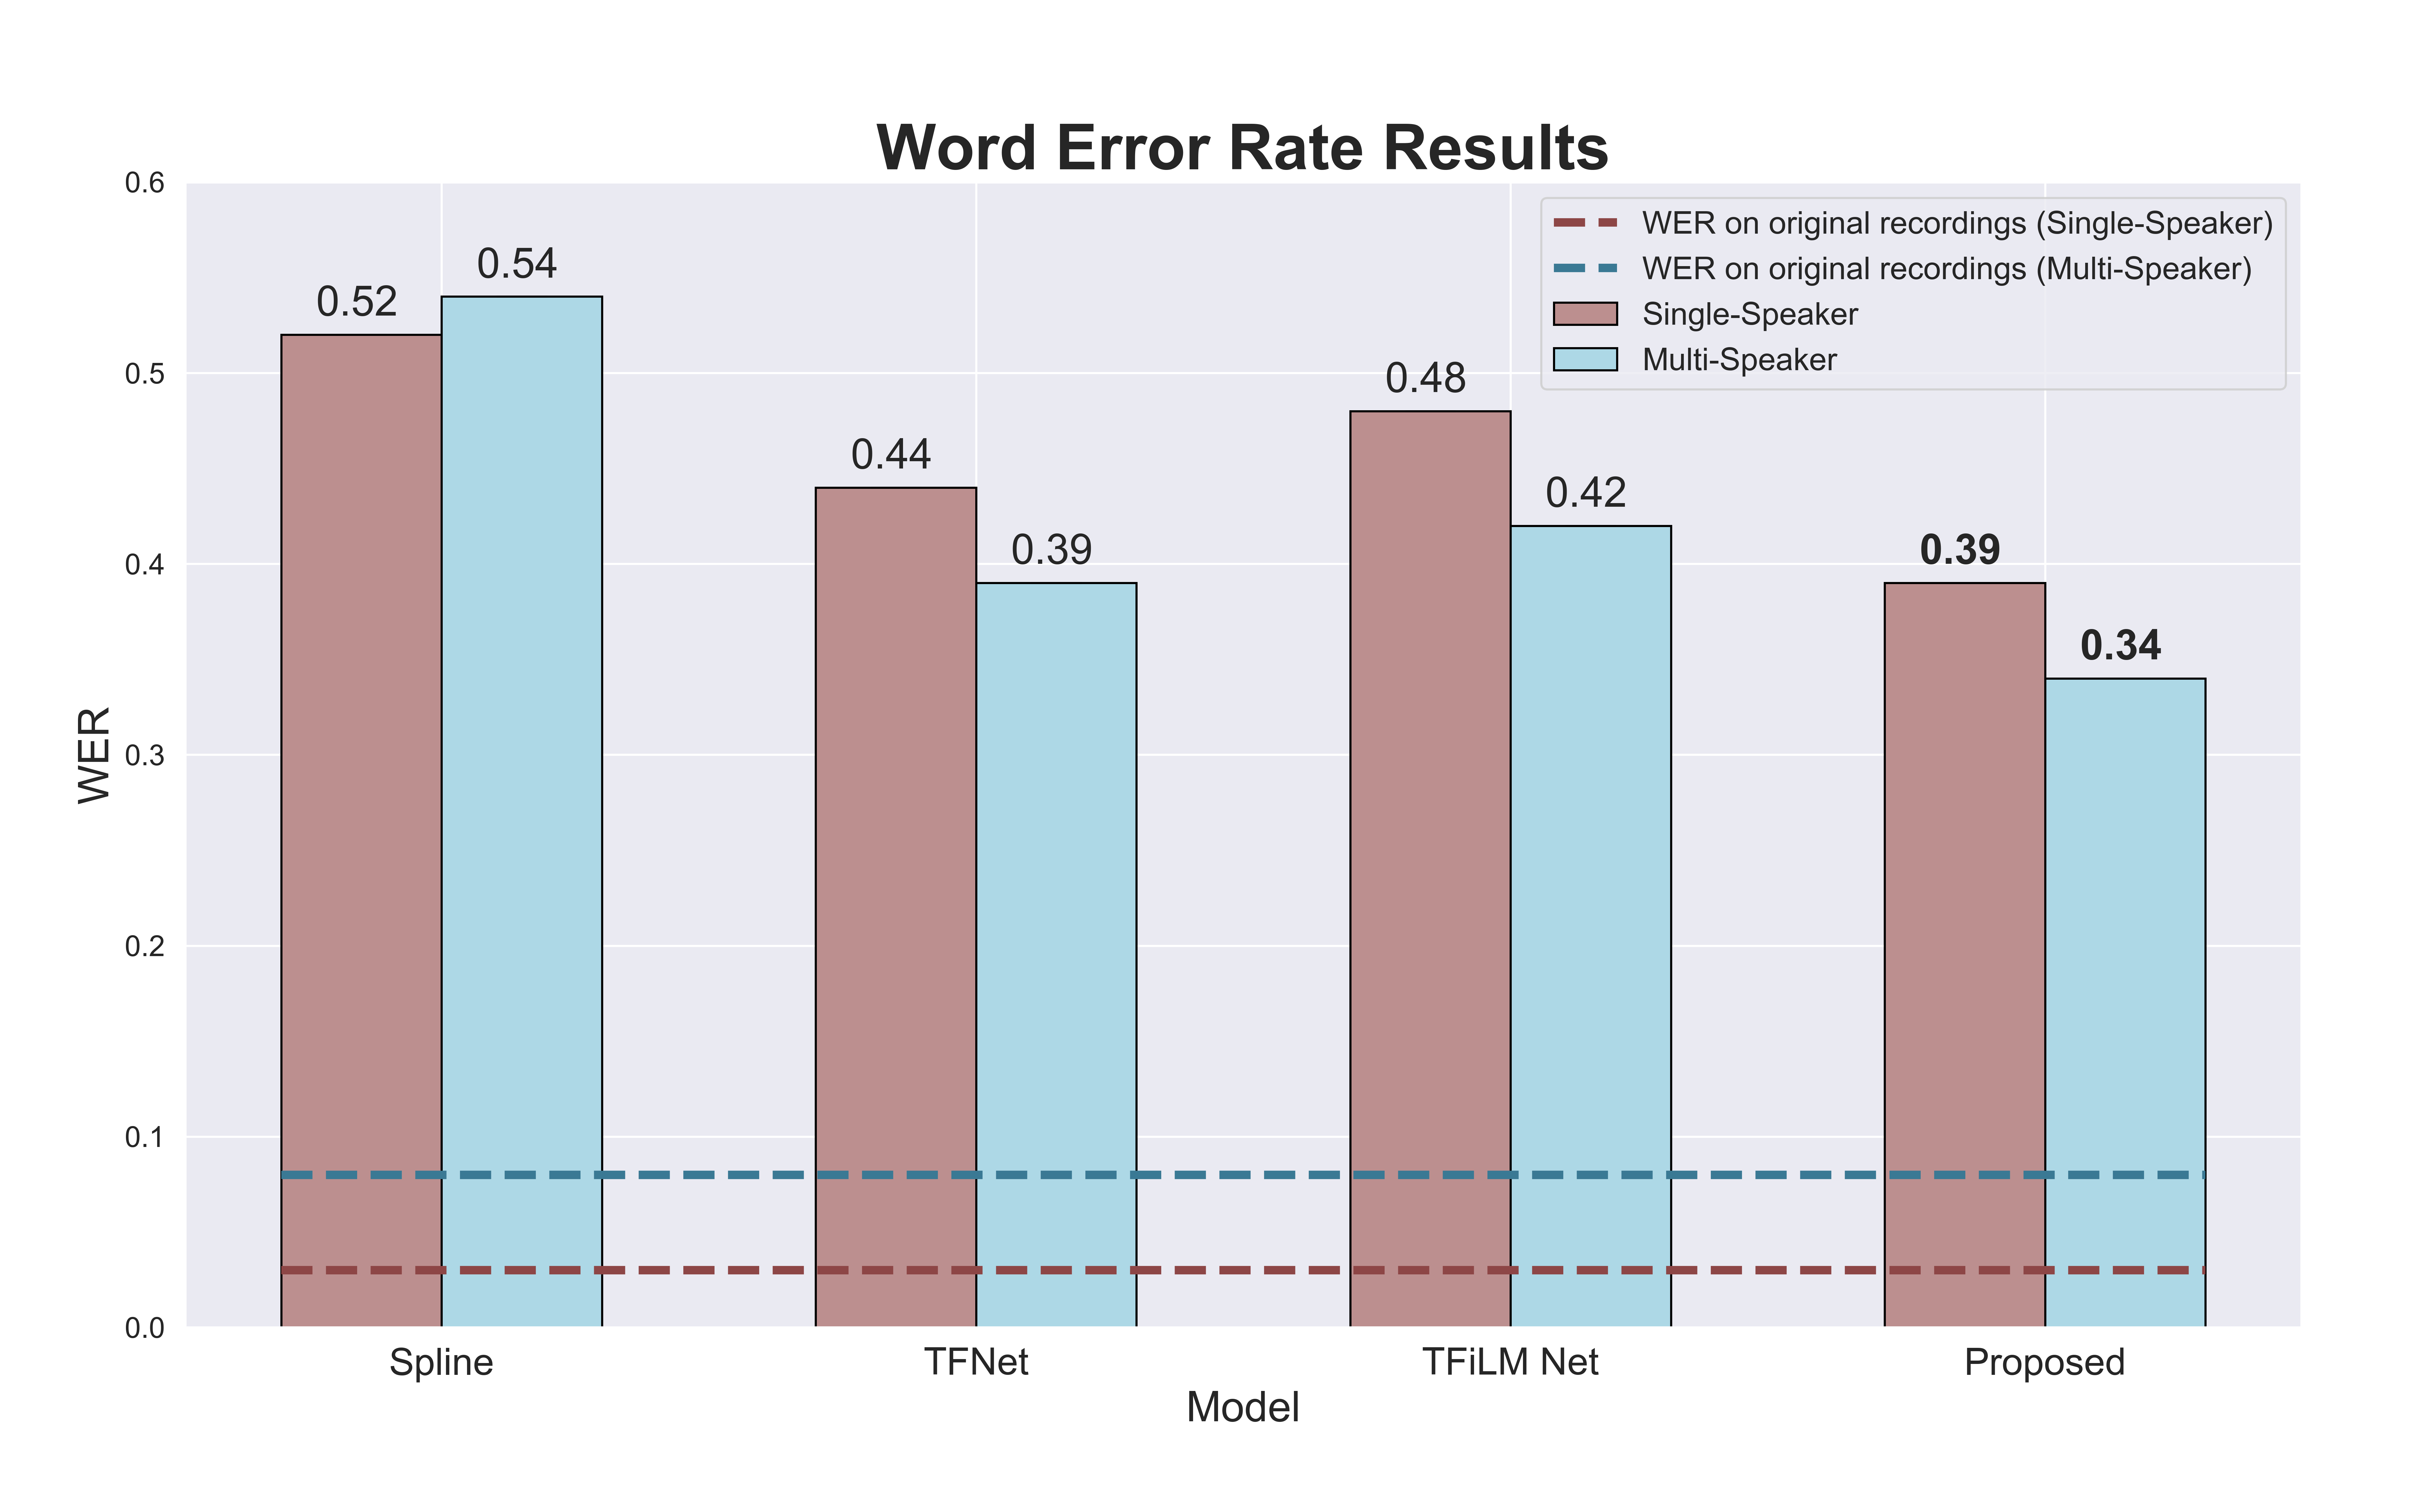
\includegraphics[scale=0.4]{img/wer_results.png}
		\caption{\gls{wer} results (in percentage) on Test Set for both Single-Speaker and Multi-Speaker tasks. \gls{wer} on original recordings is, respectively, equal to 0.03 and 0.08. Lower is better.}
		\label{fig:wer}
	\end{center}
\end{figure}

\noindent Therefore, it is fair to say that the proposed approach and the \gls{tfnet} system are the best model according to these quantitative metrics. There is not a clear winner, since the best model changes according to the considered metric. Thus, although \gls{tfnet} achieves the best \gls{snr}, the proposed model shows a better reconstruction quality in the frequency domain. Furthermore, our approach is the one which better helps the Deep Speech engine in converting audio data to text. This latter result is in agreement with the \gls{lsd} metric evaluation, and suggests that the proposed method provides a better speech quality. \\
Finally, it is worth observing the audio spectrograms. They show ~-~ from up to down in figures \ref{fig:original_signal_spec} \ref{fig:lowres_signal_spec}, \ref{fig:model_signal_spec} ~-~ a high-resolution signal, its low-resolution version obtained using spline interpolation, and the output of our model. These examples refer to an audio file that belong to the test set of the Multi-Speaker task (speaker ID and audio file ID are, respectively, \textit{p351} and \textit{004}).\\
It is important to mention that these spectrograms are computed using consecutive Fourier transforms; in particular, we use a \textit{Hamming} window of 512 samples with 50\% overlap.\\
As we can see, the proposed model is generally able to reconstruct a remarkable part of the original signal’s spectral content, especially in the frequency range 2 - 4 k\gls{hz}. It is worth noting that its estimation is mainly focused on the speech frames rather than the silence ones and this makes perfect sense. 

\begin{figure}[!htb]
	\begin{center}
		\includegraphics[scale=0.5]{img/original_signal_spec.png}
		\caption{Spectrogram showing how the frequency content of a 16kHz signal changes over time.}
		\label{fig:original_signal_spec}
	\end{center}
\end{figure}

\begin{figure}[!htb]
	\begin{center}
		\includegraphics[scale=0.5]{img/lowres_signal_spec.png}
		\caption{Spectrogram showing the spline reconstruction of the signal.}
		\label{fig:lowres_signal_spec}
	\end{center}
\end{figure}

\begin{figure}[!htb]
	\begin{center}
		\includegraphics[scale=0.5]{img/model_signal_spec.png}
		\caption{Spectrogram showing the model reconstruction of the signal.}
		\label{fig:model_signal_spec}
	\end{center}
\end{figure}

\subsubsection{Spectral Fusion Layer Weights Analysis}
We perform an additional analysis on the weights $w$ introduced in the Spectral Fusion Layer (see Equation \ref{eq:spectralfusion1}). In particular, we remind that $w$ is a trainable vector which establish the weight of each branch for the spectral magnitude prediction; the higher its values are, the more the weight of the time branch is important in the spectral magnitude $M$ calculation. Our goal is to investigate how these weights are distributed on both the proposed model and the \gls{tfnet} system.\\
This analysis is only performed for the Multi-Speaker task; however, it is reasonable to assume that the results are not very different in the Single-Speaker task since the models are trained using a fine-tuning approach. \\
The resulted distribution for both the proposed and the \gls{tfnet} models is provided in Figure \ref{fig:weights_results}. \\
\begin{figure}[H]
	\begin{center}
		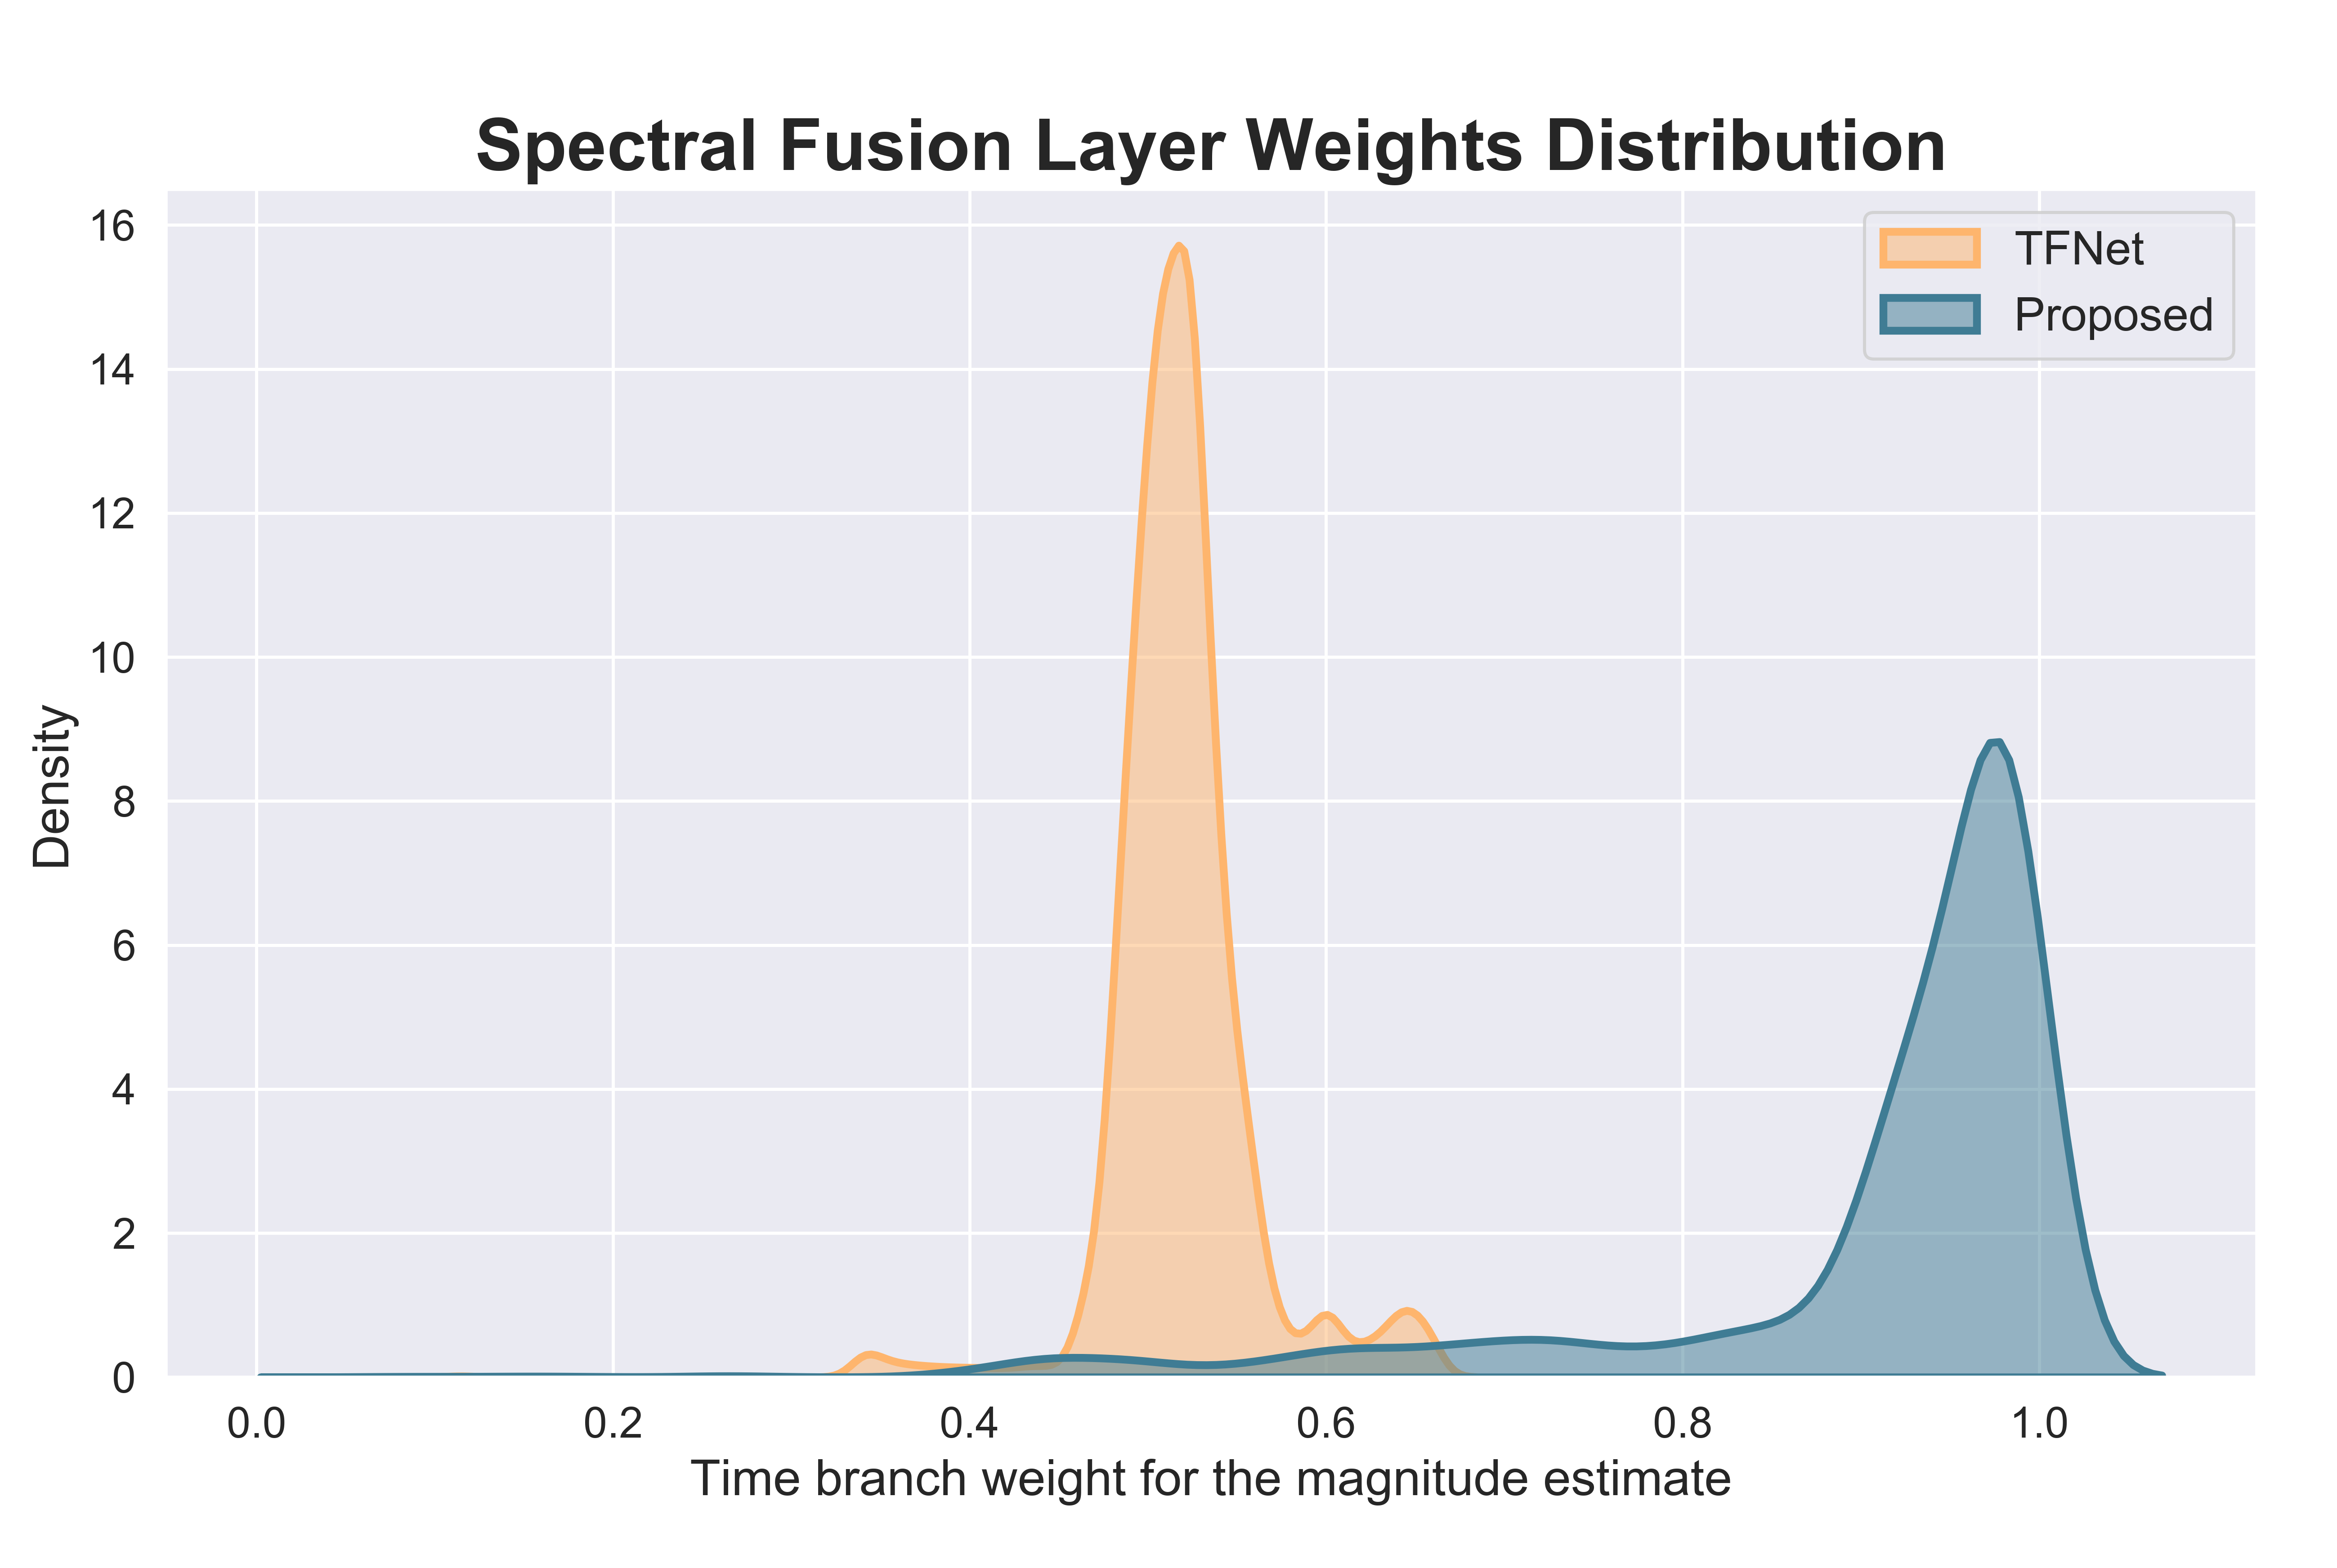
\includegraphics[scale=0.62]{img/weights_results.png}
		\caption{Spectral Fusion Layer weights distribution for both the \gls{tfnet} model and the proposed system.}
		\label{fig:weights_results}
	\end{center}
\end{figure}
\noindent As we can see, the weights of the two branches are more balanced in the \gls{tfnet} system than in the proposed model. In fact, the two means are, respectively, $\widebar{w}_{TFNet} \approx 0.5$ and  $\widebar{w}_{Proposed} \approx 0.9$. \\
Consequently, it is fair to say that, on average, for the \gls{tfnet} system the two branches contributes equally to the spectral magnitude $M$ estimation. On the other hand, for our model the two branches contribution is heavily skewed. \\
Although we cannot prove it mathematically, it is reasonable to think that this is a limitation for our model. In fact, the spectral branch, whose only goal is to contribute to the estimate of $M$, turns out not to be relevant in the final prediction. In other words, since the phase estimation is strictly time-branch dependent, the spectral branch in our model results to be almost irrelevant for the \gls{hr} reconstruction. \\
 %read tex file from chapters folder 

\chapter{Conclusions and Further Work} \label{chap:conclusions}
In this thesis we faced the problem of audio super-resolution, i.e. the task of increasing the sampling rate of a given input signal by predicting its missing high-frequency content. More specifically, we aimed to estimate a complex non-linear regression function which maps a given low-resolution input signal to its corresponding high-resolution version. \\
In order to do so, we focused our attention on deep learning models, which have demonstrated state of-the-art results in many signal processing based applications. More specifically, we worked in a supervised learning setting in which we trained models on a dataset composed by low-resolution, high-resolution 8192-length recording pairs. Input sequences were obtained by downsampling the original signals by a factor of 4; for 16 k\gls{hz} high-resolution data, this corresponds to patches of approximately 500ms. \\
Data were taken from the \gls{vctk} Corpus, which is a benchmark dataset for this task; briefly, it encompasses dozens of different speakers with various accents. \\
The proposed model is based on an hybrid architecture that combines two different methods that achieved remarkable results in literature: \gls{tfnet} and \gls{tfilm} Net. \\
The former system aims to estimate the high-frequency content of an input signal through a branching architecture; authors proposed a model which utilizes both time and frequency domain, in two different branches. In other words, \gls{tfnet} is an end-to-end system which allows the two domains to be jointly optimized. In the original paper it was demonstrated the superior performance of this strategy with respect to models which operate only in either time or frequency domain. \\
On the other hand, \gls{tfilm} Net is a deep neural network which learns the low-resolution to high-resolution mapping directly in the time domain. Its main contribution lies in the integration of convolutional and recurrent approaches to efficiently incorporate long-range information. More specifically, \gls{tfilm} layers modulate the activations of a convolutional layer through a \gls{rnn}. This system resulted very effective when processing sequential data, such as audio signals. \\
The proposed model can be considered as a mix of these two methods. On one hand, the proposed system maintains the branching structure of \gls{tfnet} which allows to process audio in both the time and the frequency domain. On the other hand, our model uses \gls{tfilm} Net modules to process data in the two branches. By doing so, we inherited the advantages of the two methods, such as the branching structure and the adoption of recurrent layers which can expand the limited receptive field of \gls{cnn}s. \\
The available resources did not allow to train, validate and test all the models in their original form: therefore, convolutional layers dimension were reduced such that each model shares the same number of trainable parameters. \\
As stated in Chapter \ref{chap:exp_results}, all the training configurations, such as the learning rate, the batch size and the optimizer, were taken from the reference papers \cite{lim2018time}, \cite{birnbaum2019temporal}. \\
As for the evaluation methods, we used two standard metrics for this task, such as \gls{snr} and \gls{lsd}, and a third criteria which is less common: we investigated whether super-resolution models can help a speech-to-text engine in better performing its automated conversion task. We investigated the effect of the three models by the use of a standard evaluation metric for \gls{stt} task such as the \gls{wer}. As a further work, we mention that it would be interesting to include qualitative metrics based on human perception of audio quality. These would certainly be the natural complement of the objective evaluations that we proposed in this work. \\
Experimental results are quite encouraging: the proposed model outperformed previous super resolution approaches on the \gls{lsd} metric, which takes into account the reconstruction quality in the spectral domain. On the other hand, we have \gls{snr}, which measures the difference between the model signal reconstruction and the ground-truth data in the time domain; according to this metric \gls{tfnet} was the system which achieves the best value. As for the \gls{wer} metric, our model showed actual improvements in helping the Deep Speech engine in the \gls{stt} conversion. \\
These results suggest that the proposed method provides a remarkable reconstruction quality. However, our Spectral Fusion Layer weights analysis described in Chapter \ref{chap:exp_results} revealed a limitation: the frequency branch of the proposed model, whose only goal is to contribute to the spectral magnitude estimation, turned out to be only partially relevant in the final prediction. This result suggested that the architecture of this branch can be better developed to improve the performance, and this can be considered as one main improvement of our approach.\\
Furthermore, it is worth highlighting that computational limitations of the available resources were an important constraint for the achievement of better results. Thus, it would certainly be interesting to evaluate the effect of our approach without a prior drastic dimensionality reduction of both the dataset size and the models' number of parameters. \\ %read tex file from chapters folder 

\printbibliography %alla fine di tutti i capitoli stampa la bibliografia
\end{document}

